\documentclass[10pt]{article}
\usepackage[a4paper,margin=2.3cm]{geometry}
\usepackage[T1]{fontenc}
\usepackage{lmodern,microtype}
\usepackage{amsmath,amssymb}
\usepackage{graphicx,booktabs,tabularx,multirow}
\usepackage[numbers,sort&compress]{natbib}
\usepackage[hidelinks]{hyperref}
\usepackage{xcolor,caption,subcaption,float}
\usepackage{authblk}
\captionsetup{font=small,labelfont=bf}
\setlength{\parskip}{0.35em}
\setlength{\emergencystretch}{2em}
% Generated by paper/scripts/make_figures.py; do not edit.
\newcommand{\numBetaIvHi}{0.89}
\newcommand{\numBetaIvLo}{0.81}
\newcommand{\numBetaIvMedian}{0.85}
\newcommand{\numBetaOlsMedian}{0.83}
\newcommand{\numCalBestNormanMse}{0.90}
\newcommand{\numCalBestNormanPearson}{0.95}
\newcommand{\numCalBestNormanPearsonSpecific}{0.93}
\newcommand{\numCalBestNormanTopkRecall}{0.93}
\newcommand{\numCalBestReplogleKEssentialMse}{0.33}
\newcommand{\numCalBestReplogleKEssentialPearson}{0.79}
\newcommand{\numCalBestReplogleKEssentialPearsonSpecific}{0.63}
\newcommand{\numCalBestReplogleKEssentialTopkRecall}{0.84}
\newcommand{\numCalBestReplogleRpeMse}{0.48}
\newcommand{\numCalBestReplogleRpePearson}{0.72}
\newcommand{\numCalBestReplogleRpePearsonSpecific}{0.66}
\newcommand{\numCalBestReplogleRpeTopkRecall}{0.75}
\newcommand{\numCalBestTianCrispraMse}{0.11}
\newcommand{\numCalBestTianCrispraPearson}{0.67}
\newcommand{\numCalBestTianCrispraPearsonSpecific}{0.15}
\newcommand{\numCalBestTianCrispraTopkRecall}{0.46}
\newcommand{\numCalBestTianCrispriMse}{0.01}
\newcommand{\numCalBestTianCrispriPearson}{0.47}
\newcommand{\numCalBestTianCrispriPearsonSpecific}{0.01}
\newcommand{\numCalBestTianCrispriTopkRecall}{0.34}
\newcommand{\numCalNormanMse}{0.94}
\newcommand{\numCalNormanPearson}{0.95}
\newcommand{\numCalNormanPearsonSpecific}{1.00}
\newcommand{\numCalNormanSkillVsMean}{0.94}
\newcommand{\numCalNormanSpearmanSpecific}{1.00}
\newcommand{\numCalReplogleKEssentialMse}{0.34}
\newcommand{\numCalReplogleKEssentialPearson}{0.80}
\newcommand{\numCalReplogleKEssentialPearsonSpecific}{1.00}
\newcommand{\numCalReplogleKEssentialSkillVsMean}{0.34}
\newcommand{\numCalReplogleKEssentialSpearmanSpecific}{1.00}
\newcommand{\numCalReplogleRpeMse}{0.72}
\newcommand{\numCalReplogleRpePearson}{0.73}
\newcommand{\numCalReplogleRpePearsonSpecific}{1.00}
\newcommand{\numCalReplogleRpeSkillVsMean}{0.72}
\newcommand{\numCalReplogleRpeSpearmanSpecific}{1.00}
\newcommand{\numCalTianCrispraMse}{0.12}
\newcommand{\numCalTianCrispraPearson}{0.82}
\newcommand{\numCalTianCrispraPearsonSpecific}{1.00}
\newcommand{\numCalTianCrispraSkillVsMean}{0.12}
\newcommand{\numCalTianCrispraSpearmanSpecific}{1.00}
\newcommand{\numCalTianCrispriMse}{0.01}
\newcommand{\numCalTianCrispriPearson}{0.60}
\newcommand{\numCalTianCrispriPearsonSpecific}{0.68}
\newcommand{\numCalTianCrispriSkillVsMean}{0.01}
\newcommand{\numCalTianCrispriSpearmanSpecific}{0.64}
\newcommand{\numCcFracTransferDeviationScaledKToRpe}{67}
\newcommand{\numCcFracTransferDeviationScaledRpeToK}{67}
\newcommand{\numCcFracTransferRawKToRpe}{39}
\newcommand{\numCcFracTransferRawRpeToK}{2}
\newcommand{\numCcHiTransferDeviationScaledKToRpe}{0.051}
\newcommand{\numCcHiTransferDeviationScaledRpeToK}{0.043}
\newcommand{\numCcHiTransferRawKToRpe}{-0.412}
\newcommand{\numCcHiTransferRawRpeToK}{-3.348}
\newcommand{\numCcLoTransferDeviationScaledKToRpe}{0.033}
\newcommand{\numCcLoTransferDeviationScaledRpeToK}{0.023}
\newcommand{\numCcLoTransferRawKToRpe}{-0.534}
\newcommand{\numCcLoTransferRawRpeToK}{-3.974}
\newcommand{\numCcSpecTransferDeviationScaledKToRpe}{0.23}
\newcommand{\numCcSpecTransferDeviationScaledRpeToK}{0.23}
\newcommand{\numCcSpecTransferRawKToRpe}{0.29}
\newcommand{\numCcSpecTransferRawRpeToK}{0.18}
\newcommand{\numCcTransferDeviationScaledKToRpe}{0.042}
\newcommand{\numCcTransferDeviationScaledRpeToK}{0.033}
\newcommand{\numCcTransferRawKToRpe}{-0.472}
\newcommand{\numCcTransferRawRpeToK}{-3.657}
\newcommand{\numCeilBatchNorman}{0.93}
\newcommand{\numCeilBatchReplogleKEssential}{0.72}
\newcommand{\numCeilBatchReplogleRpe}{0.85}
\newcommand{\numCeilBatchTianCrispra}{0.46}
\newcommand{\numCeilBatchTianCrispri}{0.19}
\newcommand{\numCeilHalfNorman}{0.93}
\newcommand{\numCeilHalfReplogleKEssential}{0.72}
\newcommand{\numCeilHalfReplogleRpe}{0.85}
\newcommand{\numCeilHalfTianCrispra}{0.55}
\newcommand{\numCeilHalfTianCrispri}{0.19}
\newcommand{\numCovNorman}{0.86}
\newcommand{\numCovReplogleKEssential}{0.90}
\newcommand{\numCovReplogleRpe}{0.90}
\newcommand{\numCovTianCrispra}{0.88}
\newcommand{\numCovTianCrispri}{0.89}
\newcommand{\numCovTopNorman}{0.45}
\newcommand{\numCovTopReplogleKEssential}{0.35}
\newcommand{\numCovTopReplogleRpe}{0.55}
\newcommand{\numCovTopTianCrispra}{0.59}
\newcommand{\numCovTopTianCrispri}{0.69}
\newcommand{\numFracBelowOne}{72}
\newcommand{\numFracReproNorman}{93}
\newcommand{\numFracReproReplogleKEssential}{33}
\newcommand{\numFracReproReplogleRpe}{72}
\newcommand{\numFracReproTianCrispra}{8}
\newcommand{\numFracReproTianCrispri}{1}
\newcommand{\numGvSkillNormanMlpEnsemble}{0.010}
\newcommand{\numGvSkillNormanRidge}{0.007}
\newcommand{\numGvSkillReplogleKEssentialMlpEnsemble}{0.043}
\newcommand{\numGvSkillReplogleKEssentialRidge}{-0.003}
\newcommand{\numGvSkillReplogleRpeMlpEnsemble}{0.048}
\newcommand{\numGvSkillReplogleRpeRidge}{0.002}
\newcommand{\numGvSkillTianCrispraMlpEnsemble}{0.010}
\newcommand{\numGvSkillTianCrispraRidge}{-0.001}
\newcommand{\numGvSkillTianCrispriMlpEnsemble}{0.001}
\newcommand{\numGvSkillTianCrispriRidge}{-0.000}
\newcommand{\numGvSpecNormanMlpEnsemble}{0.07}
\newcommand{\numGvSpecNormanRidge}{0.14}
\newcommand{\numGvSpecReplogleKEssentialMlpEnsemble}{0.19}
\newcommand{\numGvSpecReplogleKEssentialRidge}{0.13}
\newcommand{\numGvSpecReplogleRpeMlpEnsemble}{0.18}
\newcommand{\numGvSpecReplogleRpeRidge}{0.14}
\newcommand{\numGvSpecTianCrispraMlpEnsemble}{0.08}
\newcommand{\numGvSpecTianCrispraRidge}{0.01}
\newcommand{\numGvSpecTianCrispriMlpEnsemble}{0.03}
\newcommand{\numGvSpecTianCrispriRidge}{0.01}
\newcommand{\numLcFullReplogleKEssentialGeneLoadingRidge}{0.02}
\newcommand{\numLcFullReplogleKEssentialRidge}{0.03}
\newcommand{\numLcFullReplogleRpeGeneLoadingRidge}{0.01}
\newcommand{\numLcFullReplogleRpeRidge}{0.01}
\newcommand{\numLcHundredReplogleKEssentialGeneLoadingRidge}{-0.00}
\newcommand{\numLcHundredReplogleKEssentialRidge}{0.01}
\newcommand{\numLcHundredReplogleRpeGeneLoadingRidge}{0.00}
\newcommand{\numLcHundredReplogleRpeRidge}{0.01}
\newcommand{\numLcSpecFullReplogleKEssentialGeneLoadingRidge}{0.16}
\newcommand{\numLcSpecFullReplogleKEssentialRidge}{0.16}
\newcommand{\numLcSpecFullReplogleRpeGeneLoadingRidge}{0.16}
\newcommand{\numLcSpecFullReplogleRpeRidge}{0.14}
\newcommand{\numMinCOnePHolm}{9.8e-45}
\newcommand{\numNCOneBeat}{6}
\newcommand{\numNCOneTests}{12}
\newcommand{\numNCThreeBetter}{1}
\newcommand{\numNCThreeTests}{8}
\newcommand{\numNCTwoInformative}{4}
\newcommand{\numNCTwoTests}{8}
\newcommand{\numNConfirmation}{4}
\newcommand{\numNDatasetsIncluded}{5}
\newcommand{\numNNorman}{105}
\newcommand{\numNPairs}{127}
\newcommand{\numNPerturbationsTotal}{3,426}
\newcommand{\numNReplogleKEssential}{1,663}
\newcommand{\numNReplogleRpe}{1,378}
\newcommand{\numNReproNorman}{98}
\newcommand{\numNReproReplogleKEssential}{549}
\newcommand{\numNReproReplogleRpe}{997}
\newcommand{\numNReproTianCrispra}{8}
\newcommand{\numNReproTianCrispri}{2}
\newcommand{\numNSharedKToRpe}{1061}
\newcommand{\numNSharedRpeToK}{1061}
\newcommand{\numNTianCrispra}{97}
\newcommand{\numNTianCrispri}{183}
\newcommand{\numPairMseDiffScaled}{-0.00021}
\newcommand{\numPairMseDiffScaledHi}{0.00004}
\newcommand{\numPairMseDiffScaledLo}{-0.00043}
\newcommand{\numPairinterAdditivePlusMeanResidual}{0.27}
\newcommand{\numPairinterMlpOnAdditive}{0.44}
\newcommand{\numPairinterRidgeOnAdditive}{0.44}
\newcommand{\numPairinterScaledAdditive}{0.37}
\newcommand{\numPairskillAdditive}{0.49}
\newcommand{\numPairskillAdditivePlusMeanResidual}{0.54}
\newcommand{\numPairskillMlpOnAdditive}{0.63}
\newcommand{\numPairskillRidgeOnAdditive}{0.62}
\newcommand{\numPairskillScaledAdditive}{0.60}
\newcommand{\numPairspecAdditive}{0.80}
\newcommand{\numPairspecAdditivePlusMeanResidual}{0.81}
\newcommand{\numPairspecMlpOnAdditive}{0.83}
\newcommand{\numPairspecRidgeOnAdditive}{0.83}
\newcommand{\numPairspecScaledAdditive}{0.79}
\newcommand{\numPlanShaShort}{602693ec}
\newcommand{\numPrecNormanMlpEnsemble}{0.14}
\newcommand{\numPrecNormanRidge}{0.10}
\newcommand{\numPrecReplogleKEssentialMlpEnsemble}{0.33}
\newcommand{\numPrecReplogleKEssentialRidge}{0.35}
\newcommand{\numPrecReplogleRpeMlpEnsemble}{0.34}
\newcommand{\numPrecReplogleRpeRidge}{0.35}
\newcommand{\numPrecTianCrispraMlpEnsemble}{0.05}
\newcommand{\numPrecTianCrispraRidge}{0.11}
\newcommand{\numPrecTianCrispriMlpEnsemble}{0.22}
\newcommand{\numPrecTianCrispriRidge}{0.19}
\newcommand{\numRawMeanNorman}{0.50}
\newcommand{\numRawMeanReplogleKEssential}{0.26}
\newcommand{\numRawMeanReplogleRpe}{0.46}
\newcommand{\numRawMeanTianCrispra}{0.07}
\newcommand{\numRawMeanTianCrispri}{0.00}
\newcommand{\numRepSkillNormanMlp}{-0.008}
\newcommand{\numRepSkillNormanRidge}{-0.004}
\newcommand{\numRepSkillNormanShufMlp}{-0.008}
\newcommand{\numRepSkillNormanZero}{-0.342}
\newcommand{\numRepSkillReplogleKEssentialMlp}{0.075}
\newcommand{\numRepSkillReplogleKEssentialRidge}{0.074}
\newcommand{\numRepSkillReplogleKEssentialShufMlp}{0.007}
\newcommand{\numRepSkillReplogleKEssentialZero}{-0.170}
\newcommand{\numRepSkillReplogleRpeMlp}{0.067}
\newcommand{\numRepSkillReplogleRpeRidge}{0.031}
\newcommand{\numRepSkillReplogleRpeShufMlp}{0.029}
\newcommand{\numRepSkillReplogleRpeZero}{-0.188}
\newcommand{\numRepSkillTianCrispraMlp}{-0.055}
\newcommand{\numRepSkillTianCrispraRidge}{-0.012}
\newcommand{\numRepSkillTianCrispraShufMlp}{-0.049}
\newcommand{\numRepSkillTianCrispraZero}{-0.243}
\newcommand{\numRepSkillTianCrispriMlp}{0.000}
\newcommand{\numRepSkillTianCrispriRidge}{-0.001}
\newcommand{\numRepSkillTianCrispriShufMlp}{-0.006}
\newcommand{\numRepSkillTianCrispriZero}{0.093}
\newcommand{\numRepSpecNormanMlp}{0.03}
\newcommand{\numRepSpecNormanRidge}{0.01}
\newcommand{\numRepSpecNormanShufMlp}{-0.01}
\newcommand{\numRepSpecNormanZero}{0.10}
\newcommand{\numRepSpecReplogleKEssentialMlp}{0.19}
\newcommand{\numRepSpecReplogleKEssentialRidge}{0.24}
\newcommand{\numRepSpecReplogleKEssentialShufMlp}{-0.03}
\newcommand{\numRepSpecReplogleKEssentialZero}{-0.18}
\newcommand{\numRepSpecReplogleRpeMlp}{0.19}
\newcommand{\numRepSpecReplogleRpeRidge}{0.16}
\newcommand{\numRepSpecReplogleRpeShufMlp}{0.10}
\newcommand{\numRepSpecReplogleRpeZero}{0.12}
\newcommand{\numRepSpecTianCrispraMlp}{-0.42}
\newcommand{\numRepSpecTianCrispraRidge}{-0.12}
\newcommand{\numRepSpecTianCrispraShufMlp}{-0.45}
\newcommand{\numRepSpecTianCrispraZero}{-0.15}
\newcommand{\numRepSpecTianCrispriMlp}{0.07}
\newcommand{\numRepSpecTianCrispriRidge}{0.00}
\newcommand{\numRepSpecTianCrispriShufMlp}{-0.09}
\newcommand{\numRepSpecTianCrispriZero}{0.33}
\newcommand{\numReproBatchNorman}{0.79}
\newcommand{\numReproBatchReplogleKEssential}{0.42}
\newcommand{\numReproBatchReplogleRpe}{0.61}
\newcommand{\numReproBatchTianCrispra}{0.18}
\newcommand{\numReproBatchTianCrispri}{0.02}
\newcommand{\numShufSkillNormanMlpEnsemble}{-0.008}
\newcommand{\numShufSkillNormanRidge}{-0.008}
\newcommand{\numShufSkillReplogleKEssentialMlpEnsemble}{0.026}
\newcommand{\numShufSkillReplogleKEssentialRidge}{-0.003}
\newcommand{\numShufSkillReplogleRpeMlpEnsemble}{0.033}
\newcommand{\numShufSkillReplogleRpeRidge}{-0.007}
\newcommand{\numShufSkillTianCrispraMlpEnsemble}{0.017}
\newcommand{\numShufSkillTianCrispraRidge}{-0.001}
\newcommand{\numShufSkillTianCrispriMlpEnsemble}{-0.001}
\newcommand{\numShufSkillTianCrispriRidge}{-0.001}
\newcommand{\numShufSpecNormanMlpEnsemble}{-0.01}
\newcommand{\numShufSpecNormanRidge}{-0.03}
\newcommand{\numShufSpecReplogleKEssentialMlpEnsemble}{0.12}
\newcommand{\numShufSpecReplogleKEssentialRidge}{0.06}
\newcommand{\numShufSpecReplogleRpeMlpEnsemble}{0.13}
\newcommand{\numShufSpecReplogleRpeRidge}{0.04}
\newcommand{\numShufSpecTianCrispraMlpEnsemble}{0.11}
\newcommand{\numShufSpecTianCrispraRidge}{0.01}
\newcommand{\numShufSpecTianCrispriMlpEnsemble}{0.00}
\newcommand{\numShufSpecTianCrispriRidge}{-0.00}
\newcommand{\numSinglesReliability}{0.93}
\newcommand{\numSkillHiNormanGeneLoadingRidge}{0.001}
\newcommand{\numSkillHiNormanKnn}{-0.154}
\newcommand{\numSkillHiNormanMlpEnsemble}{0.009}
\newcommand{\numSkillHiNormanRidge}{0.003}
\newcommand{\numSkillHiReplogleKEssentialGeneLoadingRidge}{0.027}
\newcommand{\numSkillHiReplogleKEssentialKnn}{-0.095}
\newcommand{\numSkillHiReplogleKEssentialMlpEnsemble}{0.061}
\newcommand{\numSkillHiReplogleKEssentialRidge}{0.034}
\newcommand{\numSkillHiReplogleRpeGeneLoadingRidge}{0.024}
\newcommand{\numSkillHiReplogleRpeKnn}{-0.101}
\newcommand{\numSkillHiReplogleRpeMlpEnsemble}{0.066}
\newcommand{\numSkillHiReplogleRpeRidge}{0.023}
\newcommand{\numSkillHiTianCrispraGeneLoadingRidge}{0.000}
\newcommand{\numSkillHiTianCrispraKnn}{-0.021}
\newcommand{\numSkillHiTianCrispraMlpEnsemble}{0.021}
\newcommand{\numSkillHiTianCrispraRidge}{-0.003}
\newcommand{\numSkillHiTianCrispriGeneLoadingRidge}{0.000}
\newcommand{\numSkillHiTianCrispriKnn}{-0.042}
\newcommand{\numSkillHiTianCrispriMlpEnsemble}{0.000}
\newcommand{\numSkillHiTianCrispriRidge}{0.000}
\newcommand{\numSkillLoNormanGeneLoadingRidge}{-0.007}
\newcommand{\numSkillLoNormanKnn}{-0.289}
\newcommand{\numSkillLoNormanMlpEnsemble}{-0.022}
\newcommand{\numSkillLoNormanRidge}{-0.010}
\newcommand{\numSkillLoReplogleKEssentialGeneLoadingRidge}{0.009}
\newcommand{\numSkillLoReplogleKEssentialKnn}{-0.128}
\newcommand{\numSkillLoReplogleKEssentialMlpEnsemble}{0.038}
\newcommand{\numSkillLoReplogleKEssentialRidge}{0.015}
\newcommand{\numSkillLoReplogleRpeGeneLoadingRidge}{-0.004}
\newcommand{\numSkillLoReplogleRpeKnn}{-0.150}
\newcommand{\numSkillLoReplogleRpeMlpEnsemble}{0.037}
\newcommand{\numSkillLoReplogleRpeRidge}{-0.002}
\newcommand{\numSkillLoTianCrispraGeneLoadingRidge}{-0.002}
\newcommand{\numSkillLoTianCrispraKnn}{-0.052}
\newcommand{\numSkillLoTianCrispraMlpEnsemble}{0.003}
\newcommand{\numSkillLoTianCrispraRidge}{-0.018}
\newcommand{\numSkillLoTianCrispriGeneLoadingRidge}{-0.000}
\newcommand{\numSkillLoTianCrispriKnn}{-0.050}
\newcommand{\numSkillLoTianCrispriMlpEnsemble}{-0.001}
\newcommand{\numSkillLoTianCrispriRidge}{-0.000}
\newcommand{\numSkillNormanGeneLoadingRidge}{-0.003}
\newcommand{\numSkillNormanKnn}{-0.221}
\newcommand{\numSkillNormanMlpEnsemble}{-0.006}
\newcommand{\numSkillNormanRidge}{-0.003}
\newcommand{\numSkillReplogleKEssentialGeneLoadingRidge}{0.018}
\newcommand{\numSkillReplogleKEssentialKnn}{-0.111}
\newcommand{\numSkillReplogleKEssentialMlpEnsemble}{0.051}
\newcommand{\numSkillReplogleKEssentialRidge}{0.025}
\newcommand{\numSkillReplogleRpeGeneLoadingRidge}{0.010}
\newcommand{\numSkillReplogleRpeKnn}{-0.125}
\newcommand{\numSkillReplogleRpeMlpEnsemble}{0.052}
\newcommand{\numSkillReplogleRpeRidge}{0.011}
\newcommand{\numSkillTianCrispraGeneLoadingRidge}{-0.001}
\newcommand{\numSkillTianCrispraKnn}{-0.036}
\newcommand{\numSkillTianCrispraMlpEnsemble}{0.012}
\newcommand{\numSkillTianCrispraRidge}{-0.010}
\newcommand{\numSkillTianCrispriGeneLoadingRidge}{-0.000}
\newcommand{\numSkillTianCrispriKnn}{-0.046}
\newcommand{\numSkillTianCrispriMlpEnsemble}{-0.001}
\newcommand{\numSkillTianCrispriRidge}{-0.000}
\newcommand{\numSpecNormanGeneLoadingRidge}{0.03}
\newcommand{\numSpecNormanKnn}{-0.03}
\newcommand{\numSpecNormanMlpEnsemble}{0.04}
\newcommand{\numSpecNormanRidge}{0.02}
\newcommand{\numSpecReplogleKEssentialGeneLoadingRidge}{0.16}
\newcommand{\numSpecReplogleKEssentialKnn}{0.11}
\newcommand{\numSpecReplogleKEssentialMlpEnsemble}{0.21}
\newcommand{\numSpecReplogleKEssentialRidge}{0.16}
\newcommand{\numSpecReplogleRpeGeneLoadingRidge}{0.16}
\newcommand{\numSpecReplogleRpeKnn}{0.08}
\newcommand{\numSpecReplogleRpeMlpEnsemble}{0.19}
\newcommand{\numSpecReplogleRpeRidge}{0.14}
\newcommand{\numSpecTianCrispraGeneLoadingRidge}{-0.03}
\newcommand{\numSpecTianCrispraKnn}{0.01}
\newcommand{\numSpecTianCrispraMlpEnsemble}{0.09}
\newcommand{\numSpecTianCrispraRidge}{-0.04}
\newcommand{\numSpecTianCrispriGeneLoadingRidge}{0.01}
\newcommand{\numSpecTianCrispriKnn}{-0.02}
\newcommand{\numSpecTianCrispriMlpEnsemble}{0.01}
\newcommand{\numSpecTianCrispriRidge}{-0.00}
\newcommand{\numZeroSkillNorman}{-0.34}
\newcommand{\numZeroSkillReplogleKEssential}{-0.00}
\newcommand{\numZeroSkillReplogleRpe}{-0.26}
\newcommand{\numZeroSkillTianCrispra}{0.24}
\newcommand{\numZeroSkillTianCrispri}{0.29}
\newcommand{\numZeroSpecNorman}{0.13}
\newcommand{\numZeroSpecReplogleKEssential}{0.14}
\newcommand{\numZeroSpecReplogleRpe}{0.16}
\newcommand{\numZeroSpecTianCrispra}{0.49}
\newcommand{\numZeroSpecTianCrispri}{0.55}

% Revision (post hoc) numbers, generated by paper/scripts/revision_outputs.py; do not edit.
\newcommand{\numCovStdNormanMlpEnsemble}{0.86}
\newcommand{\numCovStdNormanRidge}{0.86}
\newcommand{\numCovStdReplogleKEssentialMlpEnsemble}{0.90}
\newcommand{\numCovStdReplogleKEssentialRidge}{0.90}
\newcommand{\numCovStdReplogleRpeMlpEnsemble}{0.90}
\newcommand{\numCovStdReplogleRpeRidge}{0.90}
\newcommand{\numCovStdTianCrispraMlpEnsemble}{0.88}
\newcommand{\numCovStdTianCrispraRidge}{0.87}
\newcommand{\numCovStdTianCrispriMlpEnsemble}{0.89}
\newcommand{\numCovStdTianCrispriRidge}{0.89}
\newcommand{\numCovStrNormanMlpEnsemble}{0.86}
\newcommand{\numCovStrNormanRidge}{0.86}
\newcommand{\numCovStrReplogleKEssentialMlpEnsemble}{0.90}
\newcommand{\numCovStrReplogleKEssentialRidge}{0.90}
\newcommand{\numCovStrReplogleRpeMlpEnsemble}{0.90}
\newcommand{\numCovStrReplogleRpeRidge}{0.90}
\newcommand{\numCovStrTianCrispraMlpEnsemble}{0.88}
\newcommand{\numCovStrTianCrispraRidge}{0.87}
\newcommand{\numCovStrTianCrispriMlpEnsemble}{0.89}
\newcommand{\numCovStrTianCrispriRidge}{0.89}
\newcommand{\numTopStdNormanMlpEnsemble}{0.45}
\newcommand{\numTopStdNormanRidge}{0.46}
\newcommand{\numTopStdReplogleKEssentialMlpEnsemble}{0.35}
\newcommand{\numTopStdReplogleKEssentialRidge}{0.34}
\newcommand{\numTopStdReplogleRpeMlpEnsemble}{0.55}
\newcommand{\numTopStdReplogleRpeRidge}{0.57}
\newcommand{\numTopStdTianCrispraMlpEnsemble}{0.59}
\newcommand{\numTopStdTianCrispraRidge}{0.60}
\newcommand{\numTopStdTianCrispriMlpEnsemble}{0.69}
\newcommand{\numTopStdTianCrispriRidge}{0.69}
\newcommand{\numTopStrNormanMlpEnsemble}{0.47}
\newcommand{\numTopStrNormanRidge}{0.48}
\newcommand{\numTopStrReplogleKEssentialMlpEnsemble}{0.37}
\newcommand{\numTopStrReplogleKEssentialRidge}{0.36}
\newcommand{\numTopStrReplogleRpeMlpEnsemble}{0.55}
\newcommand{\numTopStrReplogleRpeRidge}{0.57}
\newcommand{\numTopStrTianCrispraMlpEnsemble}{0.62}
\newcommand{\numTopStrTianCrispraRidge}{0.62}
\newcommand{\numTopStrTianCrispriMlpEnsemble}{0.71}
\newcommand{\numTopStrTianCrispriRidge}{0.70}
\newcommand{\numAblDiffHiNormanMlpEnsembleBaselineBoth}{+0.016}
\newcommand{\numAblDiffHiNormanMlpEnsembleBaselineMeanOnly}{+0.024}
\newcommand{\numAblDiffHiNormanMlpEnsembleCoexpressionOnly}{+0.004}
\newcommand{\numAblDiffHiNormanMlpEnsembleDetectionOnly}{+0.033}
\newcommand{\numAblDiffHiNormanMlpEnsembleFullSplit}{+0.021}
\newcommand{\numAblDiffHiNormanRidgeBaselineBoth}{+0.006}
\newcommand{\numAblDiffHiNormanRidgeBaselineMeanOnly}{+0.007}
\newcommand{\numAblDiffHiNormanRidgeCoexpressionOnly}{+0.001}
\newcommand{\numAblDiffHiNormanRidgeDetectionOnly}{+0.010}
\newcommand{\numAblDiffHiNormanRidgeFullSplit}{+0.013}
\newcommand{\numAblDiffHiReplogleKEssentialMlpEnsembleBaselineBoth}{-0.010}
\newcommand{\numAblDiffHiReplogleKEssentialMlpEnsembleBaselineMeanOnly}{-0.010}
\newcommand{\numAblDiffHiReplogleKEssentialMlpEnsembleCoexpressionOnly}{+0.001}
\newcommand{\numAblDiffHiReplogleKEssentialMlpEnsembleDetectionOnly}{-0.013}
\newcommand{\numAblDiffHiReplogleKEssentialMlpEnsembleFullSplit}{+0.003}
\newcommand{\numAblDiffHiReplogleKEssentialRidgeBaselineBoth}{-0.013}
\newcommand{\numAblDiffHiReplogleKEssentialRidgeBaselineMeanOnly}{-0.013}
\newcommand{\numAblDiffHiReplogleKEssentialRidgeCoexpressionOnly}{-0.003}
\newcommand{\numAblDiffHiReplogleKEssentialRidgeDetectionOnly}{-0.016}
\newcommand{\numAblDiffHiReplogleKEssentialRidgeFullSplit}{+0.001}
\newcommand{\numAblDiffHiReplogleRpeMlpEnsembleBaselineBoth}{-0.003}
\newcommand{\numAblDiffHiReplogleRpeMlpEnsembleBaselineMeanOnly}{-0.002}
\newcommand{\numAblDiffHiReplogleRpeMlpEnsembleCoexpressionOnly}{+0.005}
\newcommand{\numAblDiffHiReplogleRpeMlpEnsembleDetectionOnly}{+0.000}
\newcommand{\numAblDiffHiReplogleRpeMlpEnsembleFullSplit}{+0.006}
\newcommand{\numAblDiffHiReplogleRpeRidgeBaselineBoth}{+0.001}
\newcommand{\numAblDiffHiReplogleRpeRidgeBaselineMeanOnly}{+0.003}
\newcommand{\numAblDiffHiReplogleRpeRidgeCoexpressionOnly}{+0.003}
\newcommand{\numAblDiffHiReplogleRpeRidgeDetectionOnly}{-0.001}
\newcommand{\numAblDiffHiReplogleRpeRidgeFullSplit}{+0.010}
\newcommand{\numAblDiffHiTianCrispraMlpEnsembleBaselineBoth}{+0.012}
\newcommand{\numAblDiffHiTianCrispraMlpEnsembleBaselineMeanOnly}{+0.010}
\newcommand{\numAblDiffHiTianCrispraMlpEnsembleCoexpressionOnly}{-0.000}
\newcommand{\numAblDiffHiTianCrispraMlpEnsembleDetectionOnly}{+0.011}
\newcommand{\numAblDiffHiTianCrispraMlpEnsembleFullSplit}{+0.010}
\newcommand{\numAblDiffHiTianCrispraRidgeBaselineBoth}{+0.016}
\newcommand{\numAblDiffHiTianCrispraRidgeBaselineMeanOnly}{+0.017}
\newcommand{\numAblDiffHiTianCrispraRidgeCoexpressionOnly}{+0.001}
\newcommand{\numAblDiffHiTianCrispraRidgeDetectionOnly}{+0.017}
\newcommand{\numAblDiffHiTianCrispraRidgeFullSplit}{+0.017}
\newcommand{\numAblDiffHiTianCrispriMlpEnsembleBaselineBoth}{-0.000}
\newcommand{\numAblDiffHiTianCrispriMlpEnsembleBaselineMeanOnly}{+0.000}
\newcommand{\numAblDiffHiTianCrispriMlpEnsembleCoexpressionOnly}{+0.001}
\newcommand{\numAblDiffHiTianCrispriMlpEnsembleDetectionOnly}{-0.000}
\newcommand{\numAblDiffHiTianCrispriMlpEnsembleFullSplit}{+0.000}
\newcommand{\numAblDiffHiTianCrispriRidgeBaselineBoth}{+0.000}
\newcommand{\numAblDiffHiTianCrispriRidgeBaselineMeanOnly}{+0.000}
\newcommand{\numAblDiffHiTianCrispriRidgeCoexpressionOnly}{+0.000}
\newcommand{\numAblDiffHiTianCrispriRidgeDetectionOnly}{+0.000}
\newcommand{\numAblDiffHiTianCrispriRidgeFullSplit}{+0.000}
\newcommand{\numAblDiffLoNormanMlpEnsembleBaselineBoth}{-0.022}
\newcommand{\numAblDiffLoNormanMlpEnsembleBaselineMeanOnly}{-0.011}
\newcommand{\numAblDiffLoNormanMlpEnsembleCoexpressionOnly}{-0.019}
\newcommand{\numAblDiffLoNormanMlpEnsembleDetectionOnly}{-0.010}
\newcommand{\numAblDiffLoNormanMlpEnsembleFullSplit}{-0.012}
\newcommand{\numAblDiffLoNormanRidgeBaselineBoth}{-0.016}
\newcommand{\numAblDiffLoNormanRidgeBaselineMeanOnly}{-0.011}
\newcommand{\numAblDiffLoNormanRidgeCoexpressionOnly}{-0.001}
\newcommand{\numAblDiffLoNormanRidgeDetectionOnly}{-0.017}
\newcommand{\numAblDiffLoNormanRidgeFullSplit}{-0.001}
\newcommand{\numAblDiffLoReplogleKEssentialMlpEnsembleBaselineBoth}{-0.027}
\newcommand{\numAblDiffLoReplogleKEssentialMlpEnsembleBaselineMeanOnly}{-0.026}
\newcommand{\numAblDiffLoReplogleKEssentialMlpEnsembleCoexpressionOnly}{-0.004}
\newcommand{\numAblDiffLoReplogleKEssentialMlpEnsembleDetectionOnly}{-0.036}
\newcommand{\numAblDiffLoReplogleKEssentialMlpEnsembleFullSplit}{-0.002}
\newcommand{\numAblDiffLoReplogleKEssentialRidgeBaselineBoth}{-0.026}
\newcommand{\numAblDiffLoReplogleKEssentialRidgeBaselineMeanOnly}{-0.028}
\newcommand{\numAblDiffLoReplogleKEssentialRidgeCoexpressionOnly}{-0.008}
\newcommand{\numAblDiffLoReplogleKEssentialRidgeDetectionOnly}{-0.033}
\newcommand{\numAblDiffLoReplogleKEssentialRidgeFullSplit}{-0.003}
\newcommand{\numAblDiffLoReplogleRpeMlpEnsembleBaselineBoth}{-0.030}
\newcommand{\numAblDiffLoReplogleRpeMlpEnsembleBaselineMeanOnly}{-0.030}
\newcommand{\numAblDiffLoReplogleRpeMlpEnsembleCoexpressionOnly}{-0.006}
\newcommand{\numAblDiffLoReplogleRpeMlpEnsembleDetectionOnly}{-0.027}
\newcommand{\numAblDiffLoReplogleRpeMlpEnsembleFullSplit}{-0.012}
\newcommand{\numAblDiffLoReplogleRpeRidgeBaselineBoth}{-0.022}
\newcommand{\numAblDiffLoReplogleRpeRidgeBaselineMeanOnly}{-0.022}
\newcommand{\numAblDiffLoReplogleRpeRidgeCoexpressionOnly}{+0.000}
\newcommand{\numAblDiffLoReplogleRpeRidgeDetectionOnly}{-0.027}
\newcommand{\numAblDiffLoReplogleRpeRidgeFullSplit}{-0.001}
\newcommand{\numAblDiffLoTianCrispraMlpEnsembleBaselineBoth}{+0.002}
\newcommand{\numAblDiffLoTianCrispraMlpEnsembleBaselineMeanOnly}{-0.001}
\newcommand{\numAblDiffLoTianCrispraMlpEnsembleCoexpressionOnly}{-0.009}
\newcommand{\numAblDiffLoTianCrispraMlpEnsembleDetectionOnly}{+0.001}
\newcommand{\numAblDiffLoTianCrispraMlpEnsembleFullSplit}{+0.000}
\newcommand{\numAblDiffLoTianCrispraRidgeBaselineBoth}{-0.001}
\newcommand{\numAblDiffLoTianCrispraRidgeBaselineMeanOnly}{+0.002}
\newcommand{\numAblDiffLoTianCrispraRidgeCoexpressionOnly}{-0.001}
\newcommand{\numAblDiffLoTianCrispraRidgeDetectionOnly}{+0.000}
\newcommand{\numAblDiffLoTianCrispraRidgeFullSplit}{+0.001}
\newcommand{\numAblDiffLoTianCrispriMlpEnsembleBaselineBoth}{-0.002}
\newcommand{\numAblDiffLoTianCrispriMlpEnsembleBaselineMeanOnly}{-0.001}
\newcommand{\numAblDiffLoTianCrispriMlpEnsembleCoexpressionOnly}{-0.001}
\newcommand{\numAblDiffLoTianCrispriMlpEnsembleDetectionOnly}{-0.002}
\newcommand{\numAblDiffLoTianCrispriMlpEnsembleFullSplit}{-0.001}
\newcommand{\numAblDiffLoTianCrispriRidgeBaselineBoth}{-0.000}
\newcommand{\numAblDiffLoTianCrispriRidgeBaselineMeanOnly}{-0.000}
\newcommand{\numAblDiffLoTianCrispriRidgeCoexpressionOnly}{-0.000}
\newcommand{\numAblDiffLoTianCrispriRidgeDetectionOnly}{-0.000}
\newcommand{\numAblDiffLoTianCrispriRidgeFullSplit}{-0.000}
\newcommand{\numAblDiffNormanMlpEnsembleBaselineBoth}{-0.002}
\newcommand{\numAblDiffNormanMlpEnsembleBaselineMeanOnly}{+0.007}
\newcommand{\numAblDiffNormanMlpEnsembleCoexpressionOnly}{-0.008}
\newcommand{\numAblDiffNormanMlpEnsembleDetectionOnly}{+0.011}
\newcommand{\numAblDiffNormanMlpEnsembleFullSplit}{+0.004}
\newcommand{\numAblDiffNormanRidgeBaselineBoth}{-0.005}
\newcommand{\numAblDiffNormanRidgeBaselineMeanOnly}{-0.002}
\newcommand{\numAblDiffNormanRidgeCoexpressionOnly}{+0.000}
\newcommand{\numAblDiffNormanRidgeDetectionOnly}{-0.004}
\newcommand{\numAblDiffNormanRidgeFullSplit}{+0.006}
\newcommand{\numAblDiffReplogleKEssentialMlpEnsembleBaselineBoth}{-0.018}
\newcommand{\numAblDiffReplogleKEssentialMlpEnsembleBaselineMeanOnly}{-0.018}
\newcommand{\numAblDiffReplogleKEssentialMlpEnsembleCoexpressionOnly}{-0.001}
\newcommand{\numAblDiffReplogleKEssentialMlpEnsembleDetectionOnly}{-0.024}
\newcommand{\numAblDiffReplogleKEssentialMlpEnsembleFullSplit}{+0.001}
\newcommand{\numAblDiffReplogleKEssentialRidgeBaselineBoth}{-0.019}
\newcommand{\numAblDiffReplogleKEssentialRidgeBaselineMeanOnly}{-0.021}
\newcommand{\numAblDiffReplogleKEssentialRidgeCoexpressionOnly}{-0.005}
\newcommand{\numAblDiffReplogleKEssentialRidgeDetectionOnly}{-0.025}
\newcommand{\numAblDiffReplogleKEssentialRidgeFullSplit}{-0.001}
\newcommand{\numAblDiffReplogleRpeMlpEnsembleBaselineBoth}{-0.017}
\newcommand{\numAblDiffReplogleRpeMlpEnsembleBaselineMeanOnly}{-0.016}
\newcommand{\numAblDiffReplogleRpeMlpEnsembleCoexpressionOnly}{-0.001}
\newcommand{\numAblDiffReplogleRpeMlpEnsembleDetectionOnly}{-0.013}
\newcommand{\numAblDiffReplogleRpeMlpEnsembleFullSplit}{-0.003}
\newcommand{\numAblDiffReplogleRpeRidgeBaselineBoth}{-0.011}
\newcommand{\numAblDiffReplogleRpeRidgeBaselineMeanOnly}{-0.010}
\newcommand{\numAblDiffReplogleRpeRidgeCoexpressionOnly}{+0.001}
\newcommand{\numAblDiffReplogleRpeRidgeDetectionOnly}{-0.014}
\newcommand{\numAblDiffReplogleRpeRidgeFullSplit}{+0.004}
\newcommand{\numAblDiffTianCrispraMlpEnsembleBaselineBoth}{+0.007}
\newcommand{\numAblDiffTianCrispraMlpEnsembleBaselineMeanOnly}{+0.005}
\newcommand{\numAblDiffTianCrispraMlpEnsembleCoexpressionOnly}{-0.005}
\newcommand{\numAblDiffTianCrispraMlpEnsembleDetectionOnly}{+0.006}
\newcommand{\numAblDiffTianCrispraMlpEnsembleFullSplit}{+0.005}
\newcommand{\numAblDiffTianCrispraRidgeBaselineBoth}{+0.007}
\newcommand{\numAblDiffTianCrispraRidgeBaselineMeanOnly}{+0.008}
\newcommand{\numAblDiffTianCrispraRidgeCoexpressionOnly}{+0.000}
\newcommand{\numAblDiffTianCrispraRidgeDetectionOnly}{+0.008}
\newcommand{\numAblDiffTianCrispraRidgeFullSplit}{+0.009}
\newcommand{\numAblDiffTianCrispriMlpEnsembleBaselineBoth}{-0.001}
\newcommand{\numAblDiffTianCrispriMlpEnsembleBaselineMeanOnly}{-0.001}
\newcommand{\numAblDiffTianCrispriMlpEnsembleCoexpressionOnly}{-0.000}
\newcommand{\numAblDiffTianCrispriMlpEnsembleDetectionOnly}{-0.001}
\newcommand{\numAblDiffTianCrispriMlpEnsembleFullSplit}{-0.000}
\newcommand{\numAblDiffTianCrispriRidgeBaselineBoth}{+0.000}
\newcommand{\numAblDiffTianCrispriRidgeBaselineMeanOnly}{-0.000}
\newcommand{\numAblDiffTianCrispriRidgeCoexpressionOnly}{+0.000}
\newcommand{\numAblDiffTianCrispriRidgeDetectionOnly}{+0.000}
\newcommand{\numAblDiffTianCrispriRidgeFullSplit}{-0.000}
\newcommand{\numAblNormanMlpEnsembleBaselineBoth}{-0.008}
\newcommand{\numAblNormanMlpEnsembleBaselineMeanOnly}{0.001}
\newcommand{\numAblNormanMlpEnsembleCoexpressionOnly}{-0.014}
\newcommand{\numAblNormanMlpEnsembleDetectionOnly}{0.005}
\newcommand{\numAblNormanMlpEnsembleFull}{-0.006}
\newcommand{\numAblNormanMlpEnsembleFullSplit}{-0.002}
\newcommand{\numAblNormanRidgeBaselineBoth}{-0.008}
\newcommand{\numAblNormanRidgeBaselineMeanOnly}{-0.005}
\newcommand{\numAblNormanRidgeCoexpressionOnly}{-0.003}
\newcommand{\numAblNormanRidgeDetectionOnly}{-0.007}
\newcommand{\numAblNormanRidgeFull}{-0.003}
\newcommand{\numAblNormanRidgeFullSplit}{0.002}
\newcommand{\numAblReplogleKEssentialMlpEnsembleBaselineBoth}{0.033}
\newcommand{\numAblReplogleKEssentialMlpEnsembleBaselineMeanOnly}{0.033}
\newcommand{\numAblReplogleKEssentialMlpEnsembleCoexpressionOnly}{0.049}
\newcommand{\numAblReplogleKEssentialMlpEnsembleDetectionOnly}{0.026}
\newcommand{\numAblReplogleKEssentialMlpEnsembleFull}{0.051}
\newcommand{\numAblReplogleKEssentialMlpEnsembleFullSplit}{0.052}
\newcommand{\numAblReplogleKEssentialRidgeBaselineBoth}{0.006}
\newcommand{\numAblReplogleKEssentialRidgeBaselineMeanOnly}{0.004}
\newcommand{\numAblReplogleKEssentialRidgeCoexpressionOnly}{0.020}
\newcommand{\numAblReplogleKEssentialRidgeDetectionOnly}{0.000}
\newcommand{\numAblReplogleKEssentialRidgeFull}{0.025}
\newcommand{\numAblReplogleKEssentialRidgeFullSplit}{0.024}
\newcommand{\numAblReplogleRpeMlpEnsembleBaselineBoth}{0.035}
\newcommand{\numAblReplogleRpeMlpEnsembleBaselineMeanOnly}{0.036}
\newcommand{\numAblReplogleRpeMlpEnsembleCoexpressionOnly}{0.051}
\newcommand{\numAblReplogleRpeMlpEnsembleDetectionOnly}{0.038}
\newcommand{\numAblReplogleRpeMlpEnsembleFull}{0.052}
\newcommand{\numAblReplogleRpeMlpEnsembleFullSplit}{0.048}
\newcommand{\numAblReplogleRpeRidgeBaselineBoth}{-0.000}
\newcommand{\numAblReplogleRpeRidgeBaselineMeanOnly}{0.001}
\newcommand{\numAblReplogleRpeRidgeCoexpressionOnly}{0.012}
\newcommand{\numAblReplogleRpeRidgeDetectionOnly}{-0.004}
\newcommand{\numAblReplogleRpeRidgeFull}{0.011}
\newcommand{\numAblReplogleRpeRidgeFullSplit}{0.015}
\newcommand{\numAblSpecNormanMlpEnsembleBaselineBoth}{0.01}
\newcommand{\numAblSpecNormanMlpEnsembleBaselineMeanOnly}{0.04}
\newcommand{\numAblSpecNormanMlpEnsembleCoexpressionOnly}{-0.00}
\newcommand{\numAblSpecNormanMlpEnsembleDetectionOnly}{0.05}
\newcommand{\numAblSpecNormanMlpEnsembleFull}{0.04}
\newcommand{\numAblSpecNormanMlpEnsembleFullSplit}{0.02}
\newcommand{\numAblSpecNormanRidgeBaselineBoth}{-0.02}
\newcommand{\numAblSpecNormanRidgeBaselineMeanOnly}{-0.01}
\newcommand{\numAblSpecNormanRidgeCoexpressionOnly}{0.01}
\newcommand{\numAblSpecNormanRidgeDetectionOnly}{-0.01}
\newcommand{\numAblSpecNormanRidgeFull}{0.02}
\newcommand{\numAblSpecNormanRidgeFullSplit}{0.03}
\newcommand{\numAblSpecReplogleKEssentialMlpEnsembleBaselineBoth}{0.16}
\newcommand{\numAblSpecReplogleKEssentialMlpEnsembleBaselineMeanOnly}{0.16}
\newcommand{\numAblSpecReplogleKEssentialMlpEnsembleCoexpressionOnly}{0.21}
\newcommand{\numAblSpecReplogleKEssentialMlpEnsembleDetectionOnly}{0.15}
\newcommand{\numAblSpecReplogleKEssentialMlpEnsembleFull}{0.21}
\newcommand{\numAblSpecReplogleKEssentialMlpEnsembleFullSplit}{0.21}
\newcommand{\numAblSpecReplogleKEssentialRidgeBaselineBoth}{0.09}
\newcommand{\numAblSpecReplogleKEssentialRidgeBaselineMeanOnly}{0.07}
\newcommand{\numAblSpecReplogleKEssentialRidgeCoexpressionOnly}{0.16}
\newcommand{\numAblSpecReplogleKEssentialRidgeDetectionOnly}{0.06}
\newcommand{\numAblSpecReplogleKEssentialRidgeFull}{0.16}
\newcommand{\numAblSpecReplogleKEssentialRidgeFullSplit}{0.16}
\newcommand{\numAblSpecReplogleRpeMlpEnsembleBaselineBoth}{0.16}
\newcommand{\numAblSpecReplogleRpeMlpEnsembleBaselineMeanOnly}{0.16}
\newcommand{\numAblSpecReplogleRpeMlpEnsembleCoexpressionOnly}{0.19}
\newcommand{\numAblSpecReplogleRpeMlpEnsembleDetectionOnly}{0.16}
\newcommand{\numAblSpecReplogleRpeMlpEnsembleFull}{0.19}
\newcommand{\numAblSpecReplogleRpeMlpEnsembleFullSplit}{0.19}
\newcommand{\numAblSpecReplogleRpeRidgeBaselineBoth}{0.07}
\newcommand{\numAblSpecReplogleRpeRidgeBaselineMeanOnly}{0.08}
\newcommand{\numAblSpecReplogleRpeRidgeCoexpressionOnly}{0.14}
\newcommand{\numAblSpecReplogleRpeRidgeDetectionOnly}{0.03}
\newcommand{\numAblSpecReplogleRpeRidgeFull}{0.14}
\newcommand{\numAblSpecReplogleRpeRidgeFullSplit}{0.13}
\newcommand{\numAblSpecTianCrispraMlpEnsembleBaselineBoth}{0.11}
\newcommand{\numAblSpecTianCrispraMlpEnsembleBaselineMeanOnly}{0.11}
\newcommand{\numAblSpecTianCrispraMlpEnsembleCoexpressionOnly}{0.06}
\newcommand{\numAblSpecTianCrispraMlpEnsembleDetectionOnly}{0.10}
\newcommand{\numAblSpecTianCrispraMlpEnsembleFull}{0.09}
\newcommand{\numAblSpecTianCrispraMlpEnsembleFullSplit}{0.11}
\newcommand{\numAblSpecTianCrispraRidgeBaselineBoth}{0.02}
\newcommand{\numAblSpecTianCrispraRidgeBaselineMeanOnly}{-0.02}
\newcommand{\numAblSpecTianCrispraRidgeCoexpressionOnly}{-0.04}
\newcommand{\numAblSpecTianCrispraRidgeDetectionOnly}{0.03}
\newcommand{\numAblSpecTianCrispraRidgeFull}{-0.04}
\newcommand{\numAblSpecTianCrispraRidgeFullSplit}{0.00}
\newcommand{\numAblSpecTianCrispriMlpEnsembleBaselineBoth}{-0.01}
\newcommand{\numAblSpecTianCrispriMlpEnsembleBaselineMeanOnly}{0.01}
\newcommand{\numAblSpecTianCrispriMlpEnsembleCoexpressionOnly}{-0.00}
\newcommand{\numAblSpecTianCrispriMlpEnsembleDetectionOnly}{-0.01}
\newcommand{\numAblSpecTianCrispriMlpEnsembleFull}{0.01}
\newcommand{\numAblSpecTianCrispriMlpEnsembleFullSplit}{0.01}
\newcommand{\numAblSpecTianCrispriRidgeBaselineBoth}{-0.00}
\newcommand{\numAblSpecTianCrispriRidgeBaselineMeanOnly}{0.00}
\newcommand{\numAblSpecTianCrispriRidgeCoexpressionOnly}{0.00}
\newcommand{\numAblSpecTianCrispriRidgeDetectionOnly}{-0.01}
\newcommand{\numAblSpecTianCrispriRidgeFull}{-0.00}
\newcommand{\numAblSpecTianCrispriRidgeFullSplit}{0.01}
\newcommand{\numAblTianCrispraMlpEnsembleBaselineBoth}{0.019}
\newcommand{\numAblTianCrispraMlpEnsembleBaselineMeanOnly}{0.017}
\newcommand{\numAblTianCrispraMlpEnsembleCoexpressionOnly}{0.007}
\newcommand{\numAblTianCrispraMlpEnsembleDetectionOnly}{0.018}
\newcommand{\numAblTianCrispraMlpEnsembleFull}{0.012}
\newcommand{\numAblTianCrispraMlpEnsembleFullSplit}{0.017}
\newcommand{\numAblTianCrispraRidgeBaselineBoth}{-0.003}
\newcommand{\numAblTianCrispraRidgeBaselineMeanOnly}{-0.001}
\newcommand{\numAblTianCrispraRidgeCoexpressionOnly}{-0.009}
\newcommand{\numAblTianCrispraRidgeDetectionOnly}{-0.002}
\newcommand{\numAblTianCrispraRidgeFull}{-0.010}
\newcommand{\numAblTianCrispraRidgeFullSplit}{-0.001}
\newcommand{\numAblTianCrispriMlpEnsembleBaselineBoth}{-0.002}
\newcommand{\numAblTianCrispriMlpEnsembleBaselineMeanOnly}{-0.001}
\newcommand{\numAblTianCrispriMlpEnsembleCoexpressionOnly}{-0.001}
\newcommand{\numAblTianCrispriMlpEnsembleDetectionOnly}{-0.002}
\newcommand{\numAblTianCrispriMlpEnsembleFull}{-0.001}
\newcommand{\numAblTianCrispriMlpEnsembleFullSplit}{-0.001}
\newcommand{\numAblTianCrispriRidgeBaselineBoth}{-0.000}
\newcommand{\numAblTianCrispriRidgeBaselineMeanOnly}{-0.000}
\newcommand{\numAblTianCrispriRidgeCoexpressionOnly}{-0.000}
\newcommand{\numAblTianCrispriRidgeDetectionOnly}{-0.000}
\newcommand{\numAblTianCrispriRidgeFull}{-0.000}
\newcommand{\numAblTianCrispriRidgeFullSplit}{-0.000}
\newcommand{\numCTwoMaxHolmReplogle}{4\times10^{-8}}
\newcommand{\numCTwoMinHolmTian}{0.06}
\newcommand{\numTianAMlpFracBetter}{71}
\newcommand{\numTianAMlpMean}{-0.008}
\newcommand{\numTianAMlpMedian}{-0.028}
\newcommand{\numTianAMlpMedianHi}{-0.019}
\newcommand{\numTianAMlpMedianLo}{-0.041}
\newcommand{\numWidthRatioNormanMlpEnsemble}{1.0}
\newcommand{\numWidthRatioNormanRidge}{1.0}
\newcommand{\numWidthRatioReplogleKEssentialMlpEnsemble}{1.0}
\newcommand{\numWidthRatioReplogleKEssentialRidge}{1.0}
\newcommand{\numWidthRatioReplogleRpeMlpEnsemble}{1.0}
\newcommand{\numWidthRatioReplogleRpeRidge}{1.0}
\newcommand{\numWidthRatioTianCrispraMlpEnsemble}{1.1}
\newcommand{\numWidthRatioTianCrispraRidge}{1.0}
\newcommand{\numWidthRatioTianCrispriMlpEnsemble}{1.0}
\newcommand{\numWidthRatioTianCrispriRidge}{1.0}

% Second-revision (post hoc) numbers, generated by paper/scripts/revision2_outputs.py; do not edit.
\newcommand{\numBlockDmseHiNormanGeneLoadingRidge}{+0.015}
\newcommand{\numBlockDmseHiNormanKnn}{+0.525}
\newcommand{\numBlockDmseHiNormanMlpEnsemble}{+0.112}
\newcommand{\numBlockDmseHiNormanRidge}{+0.013}
\newcommand{\numBlockDmseHiReplogleKEssentialGeneLoadingRidge}{-0.036}
\newcommand{\numBlockDmseHiReplogleKEssentialKnn}{+0.260}
\newcommand{\numBlockDmseHiReplogleKEssentialMlpEnsemble}{-0.073}
\newcommand{\numBlockDmseHiReplogleKEssentialRidge}{-0.059}
\newcommand{\numBlockDmseHiReplogleRpeGeneLoadingRidge}{-0.098}
\newcommand{\numBlockDmseHiReplogleRpeKnn}{+0.637}
\newcommand{\numBlockDmseHiReplogleRpeMlpEnsemble}{-0.094}
\newcommand{\numBlockDmseHiReplogleRpeRidge}{-0.084}
\newcommand{\numBlockDmseHiTianCrispraGeneLoadingRidge}{+0.012}
\newcommand{\numBlockDmseHiTianCrispraKnn}{+0.140}
\newcommand{\numBlockDmseHiTianCrispraMlpEnsemble}{+0.012}
\newcommand{\numBlockDmseHiTianCrispraRidge}{+0.034}
\newcommand{\numBlockDmseHiTianCrispriGeneLoadingRidge}{+0.000}
\newcommand{\numBlockDmseHiTianCrispriKnn}{+0.087}
\newcommand{\numBlockDmseHiTianCrispriMlpEnsemble}{+0.003}
\newcommand{\numBlockDmseHiTianCrispriRidge}{+0.001}
\newcommand{\numBlockHiNormanGeneLoadingRidge}{0.001}
\newcommand{\numBlockHiNormanKnn}{-0.167}
\newcommand{\numBlockHiNormanMlpEnsemble}{0.011}
\newcommand{\numBlockHiNormanRidge}{0.001}
\newcommand{\numBlockHiReplogleKEssentialGeneLoadingRidge}{0.050}
\newcommand{\numBlockHiReplogleKEssentialKnn}{-0.073}
\newcommand{\numBlockHiReplogleKEssentialMlpEnsemble}{0.077}
\newcommand{\numBlockHiReplogleKEssentialRidge}{0.056}
\newcommand{\numBlockHiReplogleRpeGeneLoadingRidge}{0.035}
\newcommand{\numBlockHiReplogleRpeKnn}{-0.097}
\newcommand{\numBlockHiReplogleRpeMlpEnsemble}{0.082}
\newcommand{\numBlockHiReplogleRpeRidge}{0.040}
\newcommand{\numBlockHiTianCrispraGeneLoadingRidge}{0.000}
\newcommand{\numBlockHiTianCrispraKnn}{-0.025}
\newcommand{\numBlockHiTianCrispraMlpEnsemble}{0.018}
\newcommand{\numBlockHiTianCrispraRidge}{-0.004}
\newcommand{\numBlockHiTianCrispriGeneLoadingRidge}{0.000}
\newcommand{\numBlockHiTianCrispriKnn}{-0.042}
\newcommand{\numBlockHiTianCrispriMlpEnsemble}{0.001}
\newcommand{\numBlockHiTianCrispriRidge}{0.000}
\newcommand{\numBlockLoNormanGeneLoadingRidge}{-0.006}
\newcommand{\numBlockLoNormanKnn}{-0.263}
\newcommand{\numBlockLoNormanMlpEnsemble}{-0.023}
\newcommand{\numBlockLoNormanRidge}{-0.007}
\newcommand{\numBlockLoReplogleKEssentialGeneLoadingRidge}{-0.002}
\newcommand{\numBlockLoReplogleKEssentialKnn}{-0.140}
\newcommand{\numBlockLoReplogleKEssentialMlpEnsemble}{0.033}
\newcommand{\numBlockLoReplogleKEssentialRidge}{0.006}
\newcommand{\numBlockLoReplogleRpeGeneLoadingRidge}{-0.011}
\newcommand{\numBlockLoReplogleRpeKnn}{-0.149}
\newcommand{\numBlockLoReplogleRpeMlpEnsemble}{0.027}
\newcommand{\numBlockLoReplogleRpeRidge}{-0.012}
\newcommand{\numBlockLoTianCrispraGeneLoadingRidge}{-0.002}
\newcommand{\numBlockLoTianCrispraKnn}{-0.048}
\newcommand{\numBlockLoTianCrispraMlpEnsemble}{0.006}
\newcommand{\numBlockLoTianCrispraRidge}{-0.013}
\newcommand{\numBlockLoTianCrispriGeneLoadingRidge}{-0.000}
\newcommand{\numBlockLoTianCrispriKnn}{-0.050}
\newcommand{\numBlockLoTianCrispriMlpEnsemble}{-0.002}
\newcommand{\numBlockLoTianCrispriRidge}{-0.000}
\newcommand{\numCThreeFracReplogleKEssentialMlpEnsemble}{45}
\newcommand{\numCThreeFracReplogleKEssentialRidge}{41}
\newcommand{\numCThreeFracReplogleRpeMlpEnsemble}{49}
\newcommand{\numCThreeFracReplogleRpeRidge}{50}
\newcommand{\numCThreeFracTianCrispraMlpEnsemble}{41}
\newcommand{\numCThreeFracTianCrispraRidge}{56}
\newcommand{\numCThreeFracTianCrispriMlpEnsemble}{58}
\newcommand{\numCThreeFracTianCrispriRidge}{51}
\newcommand{\numCThreeMeanReplogleKEssentialMlpEnsemble}{-0.008}
\newcommand{\numCThreeMeanReplogleKEssentialRidge}{-0.029}
\newcommand{\numCThreeMeanReplogleRpeMlpEnsemble}{-0.004}
\newcommand{\numCThreeMeanReplogleRpeRidge}{-0.008}
\newcommand{\numCThreeMeanTianCrispraMlpEnsemble}{-0.002}
\newcommand{\numCThreeMeanTianCrispraRidge}{+0.008}
\newcommand{\numCThreeMeanTianCrispriMlpEnsemble}{+0.002}
\newcommand{\numCThreeMeanTianCrispriRidge}{+0.000}
\newcommand{\numCThreeMedianHiReplogleKEssentialMlpEnsemble}{-0.004}
\newcommand{\numCThreeMedianHiReplogleKEssentialRidge}{-0.013}
\newcommand{\numCThreeMedianHiReplogleRpeMlpEnsemble}{+0.004}
\newcommand{\numCThreeMedianHiReplogleRpeRidge}{+0.006}
\newcommand{\numCThreeMedianHiTianCrispraMlpEnsemble}{+0.002}
\newcommand{\numCThreeMedianHiTianCrispraRidge}{+0.004}
\newcommand{\numCThreeMedianHiTianCrispriMlpEnsemble}{+0.003}
\newcommand{\numCThreeMedianHiTianCrispriRidge}{+0.001}
\newcommand{\numCThreeMedianLoReplogleKEssentialMlpEnsemble}{-0.012}
\newcommand{\numCThreeMedianLoReplogleKEssentialRidge}{-0.021}
\newcommand{\numCThreeMedianLoReplogleRpeMlpEnsemble}{-0.011}
\newcommand{\numCThreeMedianLoReplogleRpeRidge}{-0.008}
\newcommand{\numCThreeMedianLoTianCrispraMlpEnsemble}{-0.009}
\newcommand{\numCThreeMedianLoTianCrispraRidge}{-0.001}
\newcommand{\numCThreeMedianLoTianCrispriMlpEnsemble}{+0.000}
\newcommand{\numCThreeMedianLoTianCrispriRidge}{-0.000}
\newcommand{\numCThreeMedianReplogleKEssentialMlpEnsemble}{-0.009}
\newcommand{\numCThreeMedianReplogleKEssentialRidge}{-0.017}
\newcommand{\numCThreeMedianReplogleRpeMlpEnsemble}{-0.002}
\newcommand{\numCThreeMedianReplogleRpeRidge}{-0.001}
\newcommand{\numCThreeMedianTianCrispraMlpEnsemble}{-0.003}
\newcommand{\numCThreeMedianTianCrispraRidge}{+0.002}
\newcommand{\numCThreeMedianTianCrispriMlpEnsemble}{+0.001}
\newcommand{\numCThreeMedianTianCrispriRidge}{+0.000}
\newcommand{\numCcFewestNormanGeneLoadingRidge}{0.002}
\newcommand{\numCcFewestNormanKnn}{-0.187}
\newcommand{\numCcFewestNormanMlpEnsemble}{-0.028}
\newcommand{\numCcFewestNormanRidge}{-0.009}
\newcommand{\numCcFewestReplogleKEssentialGeneLoadingRidge}{0.008}
\newcommand{\numCcFewestReplogleKEssentialKnn}{-0.080}
\newcommand{\numCcFewestReplogleKEssentialMlpEnsemble}{0.031}
\newcommand{\numCcFewestReplogleKEssentialRidge}{0.015}
\newcommand{\numCcFewestReplogleRpeGeneLoadingRidge}{0.030}
\newcommand{\numCcFewestReplogleRpeKnn}{-0.052}
\newcommand{\numCcFewestReplogleRpeMlpEnsemble}{0.025}
\newcommand{\numCcFewestReplogleRpeRidge}{0.033}
\newcommand{\numCcFewestTianCrispraGeneLoadingRidge}{-0.001}
\newcommand{\numCcFewestTianCrispraKnn}{-0.023}
\newcommand{\numCcFewestTianCrispraMlpEnsemble}{0.003}
\newcommand{\numCcFewestTianCrispraRidge}{-0.011}
\newcommand{\numCcFewestTianCrispriGeneLoadingRidge}{-0.000}
\newcommand{\numCcFewestTianCrispriKnn}{-0.043}
\newcommand{\numCcFewestTianCrispriMlpEnsemble}{-0.001}
\newcommand{\numCcFewestTianCrispriRidge}{-0.000}
\newcommand{\numCcHundredNormanGeneLoadingRidge}{-0.003}
\newcommand{\numCcHundredNormanKnn}{-0.222}
\newcommand{\numCcHundredNormanMlpEnsemble}{-0.006}
\newcommand{\numCcHundredNormanRidge}{-0.003}
\newcommand{\numCcHundredReplogleKEssentialGeneLoadingRidge}{0.023}
\newcommand{\numCcHundredReplogleKEssentialKnn}{-0.125}
\newcommand{\numCcHundredReplogleKEssentialMlpEnsemble}{0.060}
\newcommand{\numCcHundredReplogleKEssentialRidge}{0.030}
\newcommand{\numCcHundredReplogleRpeGeneLoadingRidge}{0.006}
\newcommand{\numCcHundredReplogleRpeKnn}{-0.177}
\newcommand{\numCcHundredReplogleRpeMlpEnsemble}{0.086}
\newcommand{\numCcHundredReplogleRpeRidge}{0.005}
\newcommand{\numCcHundredTianCrispraGeneLoadingRidge}{-0.001}
\newcommand{\numCcHundredTianCrispraKnn}{-0.036}
\newcommand{\numCcHundredTianCrispraMlpEnsemble}{0.012}
\newcommand{\numCcHundredTianCrispraRidge}{-0.010}
\newcommand{\numCcHundredTianCrispriGeneLoadingRidge}{-0.000}
\newcommand{\numCcHundredTianCrispriKnn}{-0.047}
\newcommand{\numCcHundredTianCrispriMlpEnsemble}{-0.001}
\newcommand{\numCcHundredTianCrispriRidge}{-0.000}
\newcommand{\numCcMostNormanGeneLoadingRidge}{-0.003}
\newcommand{\numCcMostNormanKnn}{-0.164}
\newcommand{\numCcMostNormanMlpEnsemble}{0.023}
\newcommand{\numCcMostNormanRidge}{0.010}
\newcommand{\numCcMostReplogleKEssentialGeneLoadingRidge}{0.043}
\newcommand{\numCcMostReplogleKEssentialKnn}{-0.105}
\newcommand{\numCcMostReplogleKEssentialMlpEnsemble}{0.077}
\newcommand{\numCcMostReplogleKEssentialRidge}{0.048}
\newcommand{\numCcMostReplogleRpeGeneLoadingRidge}{0.002}
\newcommand{\numCcMostReplogleRpeKnn}{-0.187}
\newcommand{\numCcMostReplogleRpeMlpEnsemble}{0.092}
\newcommand{\numCcMostReplogleRpeRidge}{0.001}
\newcommand{\numCcMostTianCrispraGeneLoadingRidge}{-0.001}
\newcommand{\numCcMostTianCrispraKnn}{-0.050}
\newcommand{\numCcMostTianCrispraMlpEnsemble}{0.017}
\newcommand{\numCcMostTianCrispraRidge}{-0.013}
\newcommand{\numCcMostTianCrispriGeneLoadingRidge}{-0.000}
\newcommand{\numCcMostTianCrispriKnn}{-0.047}
\newcommand{\numCcMostTianCrispriMlpEnsemble}{-0.001}
\newcommand{\numCcMostTianCrispriRidge}{-0.000}
\newcommand{\numCcWeightedNormanGeneLoadingRidge}{-0.003}
\newcommand{\numCcWeightedNormanKnn}{-0.214}
\newcommand{\numCcWeightedNormanMlpEnsemble}{0.004}
\newcommand{\numCcWeightedNormanRidge}{-0.000}
\newcommand{\numCcWeightedReplogleKEssentialGeneLoadingRidge}{0.002}
\newcommand{\numCcWeightedReplogleKEssentialKnn}{-0.152}
\newcommand{\numCcWeightedReplogleKEssentialMlpEnsemble}{0.020}
\newcommand{\numCcWeightedReplogleKEssentialRidge}{-0.000}
\newcommand{\numCcWeightedReplogleRpeGeneLoadingRidge}{-0.009}
\newcommand{\numCcWeightedReplogleRpeKnn}{-0.179}
\newcommand{\numCcWeightedReplogleRpeMlpEnsemble}{0.061}
\newcommand{\numCcWeightedReplogleRpeRidge}{-0.013}
\newcommand{\numCcWeightedTianCrispraGeneLoadingRidge}{-0.001}
\newcommand{\numCcWeightedTianCrispraKnn}{-0.040}
\newcommand{\numCcWeightedTianCrispraMlpEnsemble}{0.013}
\newcommand{\numCcWeightedTianCrispraRidge}{-0.010}
\newcommand{\numCcWeightedTianCrispriGeneLoadingRidge}{-0.000}
\newcommand{\numCcWeightedTianCrispriKnn}{-0.047}
\newcommand{\numCcWeightedTianCrispriMlpEnsemble}{-0.001}
\newcommand{\numCcWeightedTianCrispriRidge}{-0.000}
\newcommand{\numCsMaxNormanMlpEnsemble}{-0.002}
\newcommand{\numCsMaxNormanRidge}{-0.003}
\newcommand{\numCsMaxReplogleKEssentialMlpEnsemble}{0.052}
\newcommand{\numCsMaxReplogleKEssentialRidge}{0.025}
\newcommand{\numCsMaxReplogleRpeMlpEnsemble}{0.054}
\newcommand{\numCsMaxReplogleRpeRidge}{0.012}
\newcommand{\numCsMaxTianCrispraMlpEnsemble}{0.011}
\newcommand{\numCsMaxTianCrispraRidge}{-0.001}
\newcommand{\numCsMaxTianCrispriMlpEnsemble}{0.001}
\newcommand{\numCsMaxTianCrispriRidge}{-0.000}
\newcommand{\numCsMinNormanMlpEnsemble}{-0.010}
\newcommand{\numCsMinNormanRidge}{-0.003}
\newcommand{\numCsMinReplogleKEssentialMlpEnsemble}{0.047}
\newcommand{\numCsMinReplogleKEssentialRidge}{0.024}
\newcommand{\numCsMinReplogleRpeMlpEnsemble}{0.052}
\newcommand{\numCsMinReplogleRpeRidge}{0.010}
\newcommand{\numCsMinTianCrispraMlpEnsemble}{0.005}
\newcommand{\numCsMinTianCrispraRidge}{-0.010}
\newcommand{\numCsMinTianCrispriMlpEnsemble}{-0.004}
\newcommand{\numCsMinTianCrispriRidge}{-0.000}
\newcommand{\numGsNormanKnnExtended}{-0.218}
\newcommand{\numGsNormanKnnOutsidePrimary}{-0.226}
\newcommand{\numGsNormanKnnPrimary}{-0.221}
\newcommand{\numGsNormanKnnSilentInControls}{-0.745}
\newcommand{\numGsNormanMlpEnsembleExtended}{-0.009}
\newcommand{\numGsNormanMlpEnsembleOutsidePrimary}{-0.009}
\newcommand{\numGsNormanMlpEnsemblePrimary}{-0.010}
\newcommand{\numGsNormanMlpEnsembleSilentInControls}{-0.021}
\newcommand{\numGsNormanRidgeExtended}{-0.005}
\newcommand{\numGsNormanRidgeOutsidePrimary}{-0.006}
\newcommand{\numGsNormanRidgePrimary}{-0.003}
\newcommand{\numGsNormanRidgeSilentInControls}{-0.010}
\newcommand{\numGsReplogleKEssentialKnnExtended}{-0.108}
\newcommand{\numGsReplogleKEssentialKnnOutsidePrimary}{-0.108}
\newcommand{\numGsReplogleKEssentialKnnPrimary}{-0.111}
\newcommand{\numGsReplogleKEssentialKnnSilentInControls}{nan}
\newcommand{\numGsReplogleKEssentialMlpEnsembleExtended}{0.041}
\newcommand{\numGsReplogleKEssentialMlpEnsembleOutsidePrimary}{0.034}
\newcommand{\numGsReplogleKEssentialMlpEnsemblePrimary}{0.047}
\newcommand{\numGsReplogleKEssentialMlpEnsembleSilentInControls}{nan}
\newcommand{\numGsReplogleKEssentialRidgeExtended}{0.023}
\newcommand{\numGsReplogleKEssentialRidgeOutsidePrimary}{0.020}
\newcommand{\numGsReplogleKEssentialRidgePrimary}{0.025}
\newcommand{\numGsReplogleKEssentialRidgeSilentInControls}{nan}
\newcommand{\numGsReplogleRpeKnnExtended}{-0.120}
\newcommand{\numGsReplogleRpeKnnOutsidePrimary}{-0.122}
\newcommand{\numGsReplogleRpeKnnPrimary}{-0.125}
\newcommand{\numGsReplogleRpeKnnSilentInControls}{nan}
\newcommand{\numGsReplogleRpeMlpEnsembleExtended}{0.047}
\newcommand{\numGsReplogleRpeMlpEnsembleOutsidePrimary}{0.036}
\newcommand{\numGsReplogleRpeMlpEnsemblePrimary}{0.054}
\newcommand{\numGsReplogleRpeMlpEnsembleSilentInControls}{nan}
\newcommand{\numGsReplogleRpeRidgeExtended}{0.009}
\newcommand{\numGsReplogleRpeRidgeOutsidePrimary}{0.005}
\newcommand{\numGsReplogleRpeRidgePrimary}{0.011}
\newcommand{\numGsReplogleRpeRidgeSilentInControls}{nan}
\newcommand{\numGsSpecNormanKnnExtended}{-0.04}
\newcommand{\numGsSpecNormanKnnOutsidePrimary}{-0.04}
\newcommand{\numGsSpecNormanKnnPrimary}{-0.03}
\newcommand{\numGsSpecNormanKnnSilentInControls}{-0.03}
\newcommand{\numGsSpecNormanMlpEnsembleExtended}{0.05}
\newcommand{\numGsSpecNormanMlpEnsembleOutsidePrimary}{0.04}
\newcommand{\numGsSpecNormanMlpEnsemblePrimary}{0.05}
\newcommand{\numGsSpecNormanMlpEnsembleSilentInControls}{0.08}
\newcommand{\numGsSpecNormanRidgeExtended}{0.00}
\newcommand{\numGsSpecNormanRidgeOutsidePrimary}{-0.01}
\newcommand{\numGsSpecNormanRidgePrimary}{0.02}
\newcommand{\numGsSpecNormanRidgeSilentInControls}{-0.02}
\newcommand{\numGsSpecReplogleKEssentialKnnExtended}{0.10}
\newcommand{\numGsSpecReplogleKEssentialKnnOutsidePrimary}{0.09}
\newcommand{\numGsSpecReplogleKEssentialKnnPrimary}{0.11}
\newcommand{\numGsSpecReplogleKEssentialKnnSilentInControls}{nan}
\newcommand{\numGsSpecReplogleKEssentialMlpEnsembleExtended}{0.19}
\newcommand{\numGsSpecReplogleKEssentialMlpEnsembleOutsidePrimary}{0.17}
\newcommand{\numGsSpecReplogleKEssentialMlpEnsemblePrimary}{0.21}
\newcommand{\numGsSpecReplogleKEssentialMlpEnsembleSilentInControls}{nan}
\newcommand{\numGsSpecReplogleKEssentialRidgeExtended}{0.15}
\newcommand{\numGsSpecReplogleKEssentialRidgeOutsidePrimary}{0.14}
\newcommand{\numGsSpecReplogleKEssentialRidgePrimary}{0.16}
\newcommand{\numGsSpecReplogleKEssentialRidgeSilentInControls}{nan}
\newcommand{\numGsSpecReplogleRpeKnnExtended}{0.08}
\newcommand{\numGsSpecReplogleRpeKnnOutsidePrimary}{0.07}
\newcommand{\numGsSpecReplogleRpeKnnPrimary}{0.08}
\newcommand{\numGsSpecReplogleRpeKnnSilentInControls}{nan}
\newcommand{\numGsSpecReplogleRpeMlpEnsembleExtended}{0.18}
\newcommand{\numGsSpecReplogleRpeMlpEnsembleOutsidePrimary}{0.15}
\newcommand{\numGsSpecReplogleRpeMlpEnsemblePrimary}{0.19}
\newcommand{\numGsSpecReplogleRpeMlpEnsembleSilentInControls}{nan}
\newcommand{\numGsSpecReplogleRpeRidgeExtended}{0.13}
\newcommand{\numGsSpecReplogleRpeRidgeOutsidePrimary}{0.11}
\newcommand{\numGsSpecReplogleRpeRidgePrimary}{0.14}
\newcommand{\numGsSpecReplogleRpeRidgeSilentInControls}{nan}
\newcommand{\numGsSpecTianCrispraKnnExtended}{0.01}
\newcommand{\numGsSpecTianCrispraKnnOutsidePrimary}{0.01}
\newcommand{\numGsSpecTianCrispraKnnPrimary}{0.01}
\newcommand{\numGsSpecTianCrispraKnnSilentInControls}{-0.00}
\newcommand{\numGsSpecTianCrispraMlpEnsembleExtended}{0.05}
\newcommand{\numGsSpecTianCrispraMlpEnsembleOutsidePrimary}{0.05}
\newcommand{\numGsSpecTianCrispraMlpEnsemblePrimary}{0.08}
\newcommand{\numGsSpecTianCrispraMlpEnsembleSilentInControls}{0.03}
\newcommand{\numGsSpecTianCrispraRidgeExtended}{-0.02}
\newcommand{\numGsSpecTianCrispraRidgeOutsidePrimary}{-0.01}
\newcommand{\numGsSpecTianCrispraRidgePrimary}{-0.04}
\newcommand{\numGsSpecTianCrispraRidgeSilentInControls}{-0.01}
\newcommand{\numGsSpecTianCrispriKnnExtended}{0.00}
\newcommand{\numGsSpecTianCrispriKnnOutsidePrimary}{0.01}
\newcommand{\numGsSpecTianCrispriKnnPrimary}{-0.02}
\newcommand{\numGsSpecTianCrispriKnnSilentInControls}{-0.00}
\newcommand{\numGsSpecTianCrispriMlpEnsembleExtended}{0.00}
\newcommand{\numGsSpecTianCrispriMlpEnsembleOutsidePrimary}{0.00}
\newcommand{\numGsSpecTianCrispriMlpEnsemblePrimary}{0.00}
\newcommand{\numGsSpecTianCrispriMlpEnsembleSilentInControls}{0.03}
\newcommand{\numGsSpecTianCrispriRidgeExtended}{0.00}
\newcommand{\numGsSpecTianCrispriRidgeOutsidePrimary}{0.00}
\newcommand{\numGsSpecTianCrispriRidgePrimary}{-0.00}
\newcommand{\numGsSpecTianCrispriRidgeSilentInControls}{0.00}
\newcommand{\numGsTianCrispraKnnExtended}{-0.037}
\newcommand{\numGsTianCrispraKnnOutsidePrimary}{-0.037}
\newcommand{\numGsTianCrispraKnnPrimary}{-0.036}
\newcommand{\numGsTianCrispraKnnSilentInControls}{-0.062}
\newcommand{\numGsTianCrispraMlpEnsembleExtended}{0.004}
\newcommand{\numGsTianCrispraMlpEnsembleOutsidePrimary}{0.002}
\newcommand{\numGsTianCrispraMlpEnsemblePrimary}{0.011}
\newcommand{\numGsTianCrispraMlpEnsembleSilentInControls}{-0.001}
\newcommand{\numGsTianCrispraRidgeExtended}{-0.001}
\newcommand{\numGsTianCrispraRidgeOutsidePrimary}{-0.001}
\newcommand{\numGsTianCrispraRidgePrimary}{-0.001}
\newcommand{\numGsTianCrispraRidgeSilentInControls}{-0.001}
\newcommand{\numGsTianCrispriKnnExtended}{-0.039}
\newcommand{\numGsTianCrispriKnnOutsidePrimary}{-0.038}
\newcommand{\numGsTianCrispriKnnPrimary}{-0.046}
\newcommand{\numGsTianCrispriKnnSilentInControls}{-0.048}
\newcommand{\numGsTianCrispriMlpEnsembleExtended}{-0.002}
\newcommand{\numGsTianCrispriMlpEnsembleOutsidePrimary}{-0.002}
\newcommand{\numGsTianCrispriMlpEnsemblePrimary}{-0.001}
\newcommand{\numGsTianCrispriMlpEnsembleSilentInControls}{0.000}
\newcommand{\numGsTianCrispriRidgeExtended}{-0.000}
\newcommand{\numGsTianCrispriRidgeOutsidePrimary}{-0.000}
\newcommand{\numGsTianCrispriRidgePrimary}{-0.000}
\newcommand{\numGsTianCrispriRidgeSilentInControls}{-0.000}
\newcommand{\numIvAllNormanMlpEnsemble}{0.86}
\newcommand{\numIvAllNormanRidge}{0.86}
\newcommand{\numIvAllReplogleKEssentialMlpEnsemble}{0.90}
\newcommand{\numIvAllReplogleKEssentialRidge}{0.90}
\newcommand{\numIvAllReplogleRpeMlpEnsemble}{0.90}
\newcommand{\numIvAllReplogleRpeRidge}{0.90}
\newcommand{\numIvAllTianCrispraMlpEnsemble}{0.87}
\newcommand{\numIvAllTianCrispraRidge}{0.88}
\newcommand{\numIvAllTianCrispriMlpEnsemble}{0.89}
\newcommand{\numIvAllTianCrispriRidge}{0.89}
\newcommand{\numIvObsNormanMlpEnsemble}{0.45}
\newcommand{\numIvObsNormanRidge}{0.46}
\newcommand{\numIvObsReplogleKEssentialMlpEnsemble}{0.35}
\newcommand{\numIvObsReplogleKEssentialRidge}{0.34}
\newcommand{\numIvObsReplogleRpeMlpEnsemble}{0.55}
\newcommand{\numIvObsReplogleRpeRidge}{0.57}
\newcommand{\numIvObsTianCrispraMlpEnsemble}{0.60}
\newcommand{\numIvObsTianCrispraRidge}{0.61}
\newcommand{\numIvObsTianCrispriMlpEnsemble}{0.69}
\newcommand{\numIvObsTianCrispriRidge}{0.69}
\newcommand{\numIvPredNormanMlpEnsemble}{0.85}
\newcommand{\numIvPredNormanRidge}{0.87}
\newcommand{\numIvPredReplogleKEssentialMlpEnsemble}{0.85}
\newcommand{\numIvPredReplogleKEssentialRidge}{0.85}
\newcommand{\numIvPredReplogleRpeMlpEnsemble}{0.90}
\newcommand{\numIvPredReplogleRpeRidge}{0.90}
\newcommand{\numIvPredTianCrispraMlpEnsemble}{0.84}
\newcommand{\numIvPredTianCrispraRidge}{0.85}
\newcommand{\numIvPredTianCrispriMlpEnsemble}{0.87}
\newcommand{\numIvPredTianCrispriRidge}{0.87}
\newcommand{\numLimCellsNorman}{0.93}
\newcommand{\numLimCellsReplogleKEssential}{0.72}
\newcommand{\numLimCellsReplogleRpe}{0.85}
\newcommand{\numLimCellsTianCrispra}{0.55}
\newcommand{\numLimCellsTianCrispri}{0.19}
\newcommand{\numLimHiNorman}{0.94}
\newcommand{\numLimHiReplogleKEssential}{0.73}
\newcommand{\numLimHiReplogleRpe}{0.86}
\newcommand{\numLimHiTianCrispra}{0.51}
\newcommand{\numLimHiTianCrispri}{0.21}
\newcommand{\numLimLoNorman}{0.92}
\newcommand{\numLimLoReplogleKEssential}{0.71}
\newcommand{\numLimLoReplogleRpe}{0.85}
\newcommand{\numLimLoTianCrispra}{0.41}
\newcommand{\numLimLoTianCrispri}{0.16}
\newcommand{\numLimMaxNorman}{0.93}
\newcommand{\numLimMaxReplogleKEssential}{0.72}
\newcommand{\numLimMaxReplogleRpe}{0.85}
\newcommand{\numLimMaxTianCrispra}{0.46}
\newcommand{\numLimMaxTianCrispri}{0.19}
\newcommand{\numLimMinNorman}{0.93}
\newcommand{\numLimMinReplogleKEssential}{0.72}
\newcommand{\numLimMinReplogleRpe}{0.85}
\newcommand{\numLimMinTianCrispra}{0.46}
\newcommand{\numLimMinTianCrispri}{0.17}
\newcommand{\numLimNorman}{0.93}
\newcommand{\numLimReplogleKEssential}{0.72}
\newcommand{\numLimReplogleRpe}{0.85}
\newcommand{\numLimTianCrispra}{0.46}
\newcommand{\numLimTianCrispri}{0.19}
\newcommand{\numMseWinHighNorman}{1.00}
\newcommand{\numMseWinHighReplogleKEssential}{0.96}
\newcommand{\numMseWinHighReplogleRpe}{1.00}
\newcommand{\numMseWinHighTianCrispra}{0.36}
\newcommand{\numMseWinHighTianCrispri}{0.03}
\newcommand{\numMseWinLowNorman}{0.83}
\newcommand{\numMseWinLowReplogleKEssential}{0.00}
\newcommand{\numMseWinLowReplogleRpe}{0.24}
\newcommand{\numMseWinLowTianCrispra}{0.00}
\newcommand{\numMseWinLowTianCrispri}{0.00}
\newcommand{\numRiHiNormanMlpEnsembleAll}{0.007}
\newcommand{\numRiHiNormanMlpEnsembleRep}{0.010}
\newcommand{\numRiHiNormanRidgeAll}{0.004}
\newcommand{\numRiHiNormanRidgeRep}{0.007}
\newcommand{\numRiHiNormanZeroAll}{-0.208}
\newcommand{\numRiHiNormanZeroRep}{-0.190}
\newcommand{\numRiHiReplogleKEssentialMlpEnsembleAll}{0.045}
\newcommand{\numRiHiReplogleKEssentialMlpEnsembleRep}{0.135}
\newcommand{\numRiHiReplogleKEssentialRidgeAll}{0.029}
\newcommand{\numRiHiReplogleKEssentialRidgeRep}{0.124}
\newcommand{\numRiHiReplogleKEssentialZeroAll}{-0.023}
\newcommand{\numRiHiReplogleKEssentialZeroRep}{-0.169}
\newcommand{\numRiHiReplogleRpeMlpEnsembleAll}{0.053}
\newcommand{\numRiHiReplogleRpeMlpEnsembleRep}{0.070}
\newcommand{\numRiHiReplogleRpeRidgeAll}{0.022}
\newcommand{\numRiHiReplogleRpeRidgeRep}{0.049}
\newcommand{\numRiHiReplogleRpeZeroAll}{-0.194}
\newcommand{\numRiHiReplogleRpeZeroRep}{-0.191}
\newcommand{\numRiHiTianCrispraMlpEnsembleAll}{0.010}
\newcommand{\numRiHiTianCrispraMlpEnsembleRep}{-0.023}
\newcommand{\numRiHiTianCrispraRidgeAll}{0.000}
\newcommand{\numRiHiTianCrispraRidgeRep}{0.003}
\newcommand{\numRiHiTianCrispraZeroAll}{0.010}
\newcommand{\numRiHiTianCrispraZeroRep}{-0.206}
\newcommand{\numRiHiTianCrispriMlpEnsembleAll}{0.001}
\newcommand{\numRiHiTianCrispriMlpEnsembleRep}{0.007}
\newcommand{\numRiHiTianCrispriRidgeAll}{0.000}
\newcommand{\numRiHiTianCrispriRidgeRep}{-0.002}
\newcommand{\numRiHiTianCrispriZeroAll}{-0.025}
\newcommand{\numRiHiTianCrispriZeroRep}{-0.016}
\newcommand{\numRiLoNormanMlpEnsembleAll}{-0.023}
\newcommand{\numRiLoNormanMlpEnsembleRep}{-0.015}
\newcommand{\numRiLoNormanRidgeAll}{-0.008}
\newcommand{\numRiLoNormanRidgeRep}{-0.004}
\newcommand{\numRiLoNormanZeroAll}{-0.421}
\newcommand{\numRiLoNormanZeroRep}{-0.426}
\newcommand{\numRiLoReplogleKEssentialMlpEnsembleAll}{0.022}
\newcommand{\numRiLoReplogleKEssentialMlpEnsembleRep}{0.043}
\newcommand{\numRiLoReplogleKEssentialRidgeAll}{0.012}
\newcommand{\numRiLoReplogleKEssentialRidgeRep}{0.050}
\newcommand{\numRiLoReplogleKEssentialZeroAll}{-0.039}
\newcommand{\numRiLoReplogleKEssentialZeroRep}{-0.191}
\newcommand{\numRiLoReplogleRpeMlpEnsembleAll}{0.032}
\newcommand{\numRiLoReplogleRpeMlpEnsembleRep}{0.036}
\newcommand{\numRiLoReplogleRpeRidgeAll}{0.001}
\newcommand{\numRiLoReplogleRpeRidgeRep}{0.020}
\newcommand{\numRiLoReplogleRpeZeroAll}{-0.262}
\newcommand{\numRiLoReplogleRpeZeroRep}{-0.296}
\newcommand{\numRiLoTianCrispraMlpEnsembleAll}{-0.005}
\newcommand{\numRiLoTianCrispraMlpEnsembleRep}{-0.048}
\newcommand{\numRiLoTianCrispraRidgeAll}{-0.004}
\newcommand{\numRiLoTianCrispraRidgeRep}{-0.000}
\newcommand{\numRiLoTianCrispraZeroAll}{-0.069}
\newcommand{\numRiLoTianCrispraZeroRep}{-0.350}
\newcommand{\numRiLoTianCrispriMlpEnsembleAll}{-0.001}
\newcommand{\numRiLoTianCrispriMlpEnsembleRep}{0.007}
\newcommand{\numRiLoTianCrispriRidgeAll}{-0.000}
\newcommand{\numRiLoTianCrispriRidgeRep}{-0.002}
\newcommand{\numRiLoTianCrispriZeroAll}{-0.043}
\newcommand{\numRiLoTianCrispriZeroRep}{-0.016}
\newcommand{\numRiNNormanMlpEnsembleAll}{105}
\newcommand{\numRiNNormanMlpEnsembleRep}{88}
\newcommand{\numRiNNormanRidgeAll}{105}
\newcommand{\numRiNNormanRidgeRep}{88}
\newcommand{\numRiNNormanZeroAll}{105}
\newcommand{\numRiNNormanZeroRep}{88}
\newcommand{\numRiNReplogleKEssentialMlpEnsembleAll}{1663}
\newcommand{\numRiNReplogleKEssentialMlpEnsembleRep}{357}
\newcommand{\numRiNReplogleKEssentialRidgeAll}{1663}
\newcommand{\numRiNReplogleKEssentialRidgeRep}{357}
\newcommand{\numRiNReplogleKEssentialZeroAll}{1663}
\newcommand{\numRiNReplogleKEssentialZeroRep}{357}
\newcommand{\numRiNReplogleRpeMlpEnsembleAll}{1378}
\newcommand{\numRiNReplogleRpeMlpEnsembleRep}{605}
\newcommand{\numRiNReplogleRpeRidgeAll}{1378}
\newcommand{\numRiNReplogleRpeRidgeRep}{605}
\newcommand{\numRiNReplogleRpeZeroAll}{1378}
\newcommand{\numRiNReplogleRpeZeroRep}{605}
\newcommand{\numRiNTianCrispraMlpEnsembleAll}{97}
\newcommand{\numRiNTianCrispraMlpEnsembleRep}{6}
\newcommand{\numRiNTianCrispraRidgeAll}{97}
\newcommand{\numRiNTianCrispraRidgeRep}{6}
\newcommand{\numRiNTianCrispraZeroAll}{97}
\newcommand{\numRiNTianCrispraZeroRep}{6}
\newcommand{\numRiNTianCrispriMlpEnsembleAll}{183}
\newcommand{\numRiNTianCrispriMlpEnsembleRep}{1}
\newcommand{\numRiNTianCrispriRidgeAll}{183}
\newcommand{\numRiNTianCrispriRidgeRep}{1}
\newcommand{\numRiNTianCrispriZeroAll}{183}
\newcommand{\numRiNTianCrispriZeroRep}{1}
\newcommand{\numRiSkillNormanMlpEnsembleAll}{-0.007}
\newcommand{\numRiSkillNormanMlpEnsembleRep}{-0.002}
\newcommand{\numRiSkillNormanRidgeAll}{-0.002}
\newcommand{\numRiSkillNormanRidgeRep}{0.001}
\newcommand{\numRiSkillNormanZeroAll}{-0.312}
\newcommand{\numRiSkillNormanZeroRep}{-0.307}
\newcommand{\numRiSkillReplogleKEssentialMlpEnsembleAll}{0.035}
\newcommand{\numRiSkillReplogleKEssentialMlpEnsembleRep}{0.094}
\newcommand{\numRiSkillReplogleKEssentialRidgeAll}{0.022}
\newcommand{\numRiSkillReplogleKEssentialRidgeRep}{0.090}
\newcommand{\numRiSkillReplogleKEssentialZeroAll}{-0.030}
\newcommand{\numRiSkillReplogleKEssentialZeroRep}{-0.180}
\newcommand{\numRiSkillReplogleRpeMlpEnsembleAll}{0.043}
\newcommand{\numRiSkillReplogleRpeMlpEnsembleRep}{0.052}
\newcommand{\numRiSkillReplogleRpeRidgeAll}{0.011}
\newcommand{\numRiSkillReplogleRpeRidgeRep}{0.035}
\newcommand{\numRiSkillReplogleRpeZeroAll}{-0.228}
\newcommand{\numRiSkillReplogleRpeZeroRep}{-0.245}
\newcommand{\numRiSkillTianCrispraMlpEnsembleAll}{0.003}
\newcommand{\numRiSkillTianCrispraMlpEnsembleRep}{-0.035}
\newcommand{\numRiSkillTianCrispraRidgeAll}{-0.002}
\newcommand{\numRiSkillTianCrispraRidgeRep}{0.001}
\newcommand{\numRiSkillTianCrispraZeroAll}{-0.029}
\newcommand{\numRiSkillTianCrispraZeroRep}{-0.278}
\newcommand{\numRiSkillTianCrispriMlpEnsembleAll}{-0.000}
\newcommand{\numRiSkillTianCrispriMlpEnsembleRep}{0.007}
\newcommand{\numRiSkillTianCrispriRidgeAll}{0.000}
\newcommand{\numRiSkillTianCrispriRidgeRep}{-0.002}
\newcommand{\numRiSkillTianCrispriZeroAll}{-0.034}
\newcommand{\numRiSkillTianCrispriZeroRep}{-0.016}
\newcommand{\numRiSpecNormanMlpEnsembleAll}{0.05}
\newcommand{\numRiSpecNormanMlpEnsembleRep}{0.05}
\newcommand{\numRiSpecNormanRidgeAll}{0.02}
\newcommand{\numRiSpecNormanRidgeRep}{0.03}
\newcommand{\numRiSpecNormanZeroAll}{0.11}
\newcommand{\numRiSpecNormanZeroRep}{0.07}
\newcommand{\numRiSpecReplogleKEssentialMlpEnsembleAll}{0.17}
\newcommand{\numRiSpecReplogleKEssentialMlpEnsembleRep}{0.22}
\newcommand{\numRiSpecReplogleKEssentialRidgeAll}{0.14}
\newcommand{\numRiSpecReplogleKEssentialRidgeRep}{0.28}
\newcommand{\numRiSpecReplogleKEssentialZeroAll}{0.09}
\newcommand{\numRiSpecReplogleKEssentialZeroRep}{-0.26}
\newcommand{\numRiSpecReplogleRpeMlpEnsembleAll}{0.16}
\newcommand{\numRiSpecReplogleRpeMlpEnsembleRep}{0.12}
\newcommand{\numRiSpecReplogleRpeRidgeAll}{0.12}
\newcommand{\numRiSpecReplogleRpeRidgeRep}{0.15}
\newcommand{\numRiSpecReplogleRpeZeroAll}{0.12}
\newcommand{\numRiSpecReplogleRpeZeroRep}{-0.03}
\newcommand{\numRiSpecTianCrispraMlpEnsembleAll}{0.04}
\newcommand{\numRiSpecTianCrispraMlpEnsembleRep}{-0.45}
\newcommand{\numRiSpecTianCrispraRidgeAll}{-0.04}
\newcommand{\numRiSpecTianCrispraRidgeRep}{0.03}
\newcommand{\numRiSpecTianCrispraZeroAll}{0.24}
\newcommand{\numRiSpecTianCrispraZeroRep}{-0.31}
\newcommand{\numRiSpecTianCrispriMlpEnsembleAll}{0.01}
\newcommand{\numRiSpecTianCrispriMlpEnsembleRep}{0.10}
\newcommand{\numRiSpecTianCrispriRidgeAll}{-0.00}
\newcommand{\numRiSpecTianCrispriRidgeRep}{-0.03}
\newcommand{\numRiSpecTianCrispriZeroAll}{0.27}
\newcommand{\numRiSpecTianCrispriZeroRep}{0.16}
\newcommand{\numRkHiNormanMlpEnsembleTen}{0.40}
\newcommand{\numRkHiNormanMlpEnsembleThirty}{0.44}
\newcommand{\numRkHiNormanMlpEnsembleTwenty}{0.38}
\newcommand{\numRkHiNormanRidgeTen}{0.30}
\newcommand{\numRkHiNormanRidgeThirty}{0.44}
\newcommand{\numRkHiNormanRidgeTwenty}{0.29}
\newcommand{\numRkHiReplogleKEssentialMlpEnsembleTen}{0.23}
\newcommand{\numRkHiReplogleKEssentialMlpEnsembleThirty}{0.48}
\newcommand{\numRkHiReplogleKEssentialMlpEnsembleTwenty}{0.39}
\newcommand{\numRkHiReplogleKEssentialRidgeTen}{0.24}
\newcommand{\numRkHiReplogleKEssentialRidgeThirty}{0.45}
\newcommand{\numRkHiReplogleKEssentialRidgeTwenty}{0.39}
\newcommand{\numRkHiReplogleRpeMlpEnsembleTen}{0.38}
\newcommand{\numRkHiReplogleRpeMlpEnsembleThirty}{0.46}
\newcommand{\numRkHiReplogleRpeMlpEnsembleTwenty}{0.39}
\newcommand{\numRkHiReplogleRpeRidgeTen}{0.38}
\newcommand{\numRkHiReplogleRpeRidgeThirty}{0.45}
\newcommand{\numRkHiReplogleRpeRidgeTwenty}{0.41}
\newcommand{\numRkHiTianCrispraMlpEnsembleTen}{0.00}
\newcommand{\numRkHiTianCrispraMlpEnsembleThirty}{0.34}
\newcommand{\numRkHiTianCrispraMlpEnsembleTwenty}{0.16}
\newcommand{\numRkHiTianCrispraRidgeTen}{0.20}
\newcommand{\numRkHiTianCrispraRidgeThirty}{0.41}
\newcommand{\numRkHiTianCrispraRidgeTwenty}{0.26}
\newcommand{\numRkHiTianCrispriMlpEnsembleTen}{0.17}
\newcommand{\numRkHiTianCrispriMlpEnsembleThirty}{0.42}
\newcommand{\numRkHiTianCrispriMlpEnsembleTwenty}{0.27}
\newcommand{\numRkHiTianCrispriRidgeTen}{0.28}
\newcommand{\numRkHiTianCrispriRidgeThirty}{0.42}
\newcommand{\numRkHiTianCrispriRidgeTwenty}{0.32}
\newcommand{\numRkLoNormanMlpEnsembleTen}{0.00}
\newcommand{\numRkLoNormanMlpEnsembleThirty}{0.16}
\newcommand{\numRkLoNormanMlpEnsembleTwenty}{0.05}
\newcommand{\numRkLoNormanRidgeTen}{0.00}
\newcommand{\numRkLoNormanRidgeThirty}{0.16}
\newcommand{\numRkLoNormanRidgeTwenty}{0.00}
\newcommand{\numRkLoReplogleKEssentialMlpEnsembleTen}{0.11}
\newcommand{\numRkLoReplogleKEssentialMlpEnsembleThirty}{0.41}
\newcommand{\numRkLoReplogleKEssentialMlpEnsembleTwenty}{0.31}
\newcommand{\numRkLoReplogleKEssentialRidgeTen}{0.12}
\newcommand{\numRkLoReplogleKEssentialRidgeThirty}{0.38}
\newcommand{\numRkLoReplogleKEssentialRidgeTwenty}{0.29}
\newcommand{\numRkLoReplogleRpeMlpEnsembleTen}{0.23}
\newcommand{\numRkLoReplogleRpeMlpEnsembleThirty}{0.38}
\newcommand{\numRkLoReplogleRpeMlpEnsembleTwenty}{0.29}
\newcommand{\numRkLoReplogleRpeRidgeTen}{0.23}
\newcommand{\numRkLoReplogleRpeRidgeThirty}{0.37}
\newcommand{\numRkLoReplogleRpeRidgeTwenty}{0.30}
\newcommand{\numRkLoTianCrispraMlpEnsembleTen}{0.00}
\newcommand{\numRkLoTianCrispraMlpEnsembleThirty}{0.07}
\newcommand{\numRkLoTianCrispraMlpEnsembleTwenty}{0.00}
\newcommand{\numRkLoTianCrispraRidgeTen}{0.00}
\newcommand{\numRkLoTianCrispraRidgeThirty}{0.10}
\newcommand{\numRkLoTianCrispraRidgeTwenty}{0.00}
\newcommand{\numRkLoTianCrispriMlpEnsembleTen}{0.00}
\newcommand{\numRkLoTianCrispriMlpEnsembleThirty}{0.22}
\newcommand{\numRkLoTianCrispriMlpEnsembleTwenty}{0.03}
\newcommand{\numRkLoTianCrispriRidgeTen}{0.00}
\newcommand{\numRkLoTianCrispriRidgeThirty}{0.22}
\newcommand{\numRkLoTianCrispriRidgeTwenty}{0.08}
\newcommand{\numRkNormanMlpEnsembleTen}{0.10}
\newcommand{\numRkNormanMlpEnsembleThirty}{0.34}
\newcommand{\numRkNormanMlpEnsembleTwenty}{0.19}
\newcommand{\numRkNormanRidgeTen}{0.10}
\newcommand{\numRkNormanRidgeThirty}{0.31}
\newcommand{\numRkNormanRidgeTwenty}{0.10}
\newcommand{\numRkPNormanMlpEnsembleTen}{0.653}
\newcommand{\numRkPNormanMlpEnsembleThirty}{0.337}
\newcommand{\numRkPNormanMlpEnsembleTwenty}{0.641}
\newcommand{\numRkPNormanRidgeTen}{0.647}
\newcommand{\numRkPNormanRidgeThirty}{0.550}
\newcommand{\numRkPNormanRidgeTwenty}{0.954}
\newcommand{\numRkPReplogleKEssentialMlpEnsembleTen}{0.002}
\newcommand{\numRkPReplogleKEssentialMlpEnsembleThirty}{0.000}
\newcommand{\numRkPReplogleKEssentialMlpEnsembleTwenty}{0.000}
\newcommand{\numRkPReplogleKEssentialRidgeTen}{0.005}
\newcommand{\numRkPReplogleKEssentialRidgeThirty}{0.000}
\newcommand{\numRkPReplogleKEssentialRidgeTwenty}{0.000}
\newcommand{\numRkPReplogleRpeMlpEnsembleTen}{0.000}
\newcommand{\numRkPReplogleRpeMlpEnsembleThirty}{0.000}
\newcommand{\numRkPReplogleRpeMlpEnsembleTwenty}{0.000}
\newcommand{\numRkPReplogleRpeRidgeTen}{0.000}
\newcommand{\numRkPReplogleRpeRidgeThirty}{0.000}
\newcommand{\numRkPReplogleRpeRidgeTwenty}{0.000}
\newcommand{\numRkPTianCrispraMlpEnsembleTen}{1.000}
\newcommand{\numRkPTianCrispraMlpEnsembleThirty}{0.853}
\newcommand{\numRkPTianCrispraMlpEnsembleTwenty}{0.986}
\newcommand{\numRkPTianCrispraRidgeTen}{1.000}
\newcommand{\numRkPTianCrispraRidgeThirty}{0.719}
\newcommand{\numRkPTianCrispraRidgeTwenty}{0.992}
\newcommand{\numRkPTianCrispriMlpEnsembleTen}{0.864}
\newcommand{\numRkPTianCrispriMlpEnsembleThirty}{0.653}
\newcommand{\numRkPTianCrispriMlpEnsembleTwenty}{0.972}
\newcommand{\numRkPTianCrispriRidgeTen}{0.567}
\newcommand{\numRkPTianCrispriRidgeThirty}{0.492}
\newcommand{\numRkPTianCrispriRidgeTwenty}{0.667}
\newcommand{\numRkReplogleKEssentialMlpEnsembleTen}{0.17}
\newcommand{\numRkReplogleKEssentialMlpEnsembleThirty}{0.44}
\newcommand{\numRkReplogleKEssentialMlpEnsembleTwenty}{0.35}
\newcommand{\numRkReplogleKEssentialRidgeTen}{0.17}
\newcommand{\numRkReplogleKEssentialRidgeThirty}{0.41}
\newcommand{\numRkReplogleKEssentialRidgeTwenty}{0.35}
\newcommand{\numRkReplogleRpeMlpEnsembleTen}{0.30}
\newcommand{\numRkReplogleRpeMlpEnsembleThirty}{0.41}
\newcommand{\numRkReplogleRpeMlpEnsembleTwenty}{0.34}
\newcommand{\numRkReplogleRpeRidgeTen}{0.31}
\newcommand{\numRkReplogleRpeRidgeThirty}{0.41}
\newcommand{\numRkReplogleRpeRidgeTwenty}{0.35}
\newcommand{\numRkSeedMaxNorman}{0.19}
\newcommand{\numRkSeedMaxReplogleKEssential}{0.33}
\newcommand{\numRkSeedMaxReplogleRpe}{0.37}
\newcommand{\numRkSeedMaxTianCrispra}{0.21}
\newcommand{\numRkSeedMaxTianCrispri}{0.24}
\newcommand{\numRkSeedMinNorman}{0.10}
\newcommand{\numRkSeedMinReplogleKEssential}{0.29}
\newcommand{\numRkSeedMinReplogleRpe}{0.34}
\newcommand{\numRkSeedMinTianCrispra}{0.05}
\newcommand{\numRkSeedMinTianCrispri}{0.08}
\newcommand{\numRkTianCrispraMlpEnsembleTen}{0.00}
\newcommand{\numRkTianCrispraMlpEnsembleThirty}{0.24}
\newcommand{\numRkTianCrispraMlpEnsembleTwenty}{0.05}
\newcommand{\numRkTianCrispraRidgeTen}{0.00}
\newcommand{\numRkTianCrispraRidgeThirty}{0.28}
\newcommand{\numRkTianCrispraRidgeTwenty}{0.05}
\newcommand{\numRkTianCrispriMlpEnsembleTen}{0.06}
\newcommand{\numRkTianCrispriMlpEnsembleThirty}{0.29}
\newcommand{\numRkTianCrispriMlpEnsembleTwenty}{0.11}
\newcommand{\numRkTianCrispriRidgeTen}{0.11}
\newcommand{\numRkTianCrispriRidgeThirty}{0.31}
\newcommand{\numRkTianCrispriRidgeTwenty}{0.19}
\newcommand{\numSeedMaxNormanMlpEnsemble}{0.011}
\newcommand{\numSeedMaxReplogleKEssentialMlpEnsemble}{0.055}
\newcommand{\numSeedMaxReplogleRpeMlpEnsemble}{0.054}
\newcommand{\numSeedMaxTianCrispraMlpEnsemble}{0.016}
\newcommand{\numSeedMaxTianCrispriMlpEnsemble}{-0.001}
\newcommand{\numSeedMinNormanMlpEnsemble}{-0.015}
\newcommand{\numSeedMinReplogleKEssentialMlpEnsemble}{0.047}
\newcommand{\numSeedMinReplogleRpeMlpEnsemble}{0.047}
\newcommand{\numSeedMinTianCrispraMlpEnsemble}{0.006}
\newcommand{\numSeedMinTianCrispriMlpEnsemble}{-0.003}
\newcommand{\numWinMeanHiNormanMse}{0.97}
\newcommand{\numWinMeanHiNormanPearson}{0.98}
\newcommand{\numWinMeanHiNormanPearsonSpecific}{1.00}
\newcommand{\numWinMeanHiNormanSpearmanSpecific}{1.00}
\newcommand{\numWinMeanHiNormanTopkRecall}{0.97}
\newcommand{\numWinMeanHiReplogleKEssentialMse}{0.36}
\newcommand{\numWinMeanHiReplogleKEssentialPearson}{0.82}
\newcommand{\numWinMeanHiReplogleKEssentialPearsonSpecific}{1.00}
\newcommand{\numWinMeanHiReplogleKEssentialSpearmanSpecific}{1.00}
\newcommand{\numWinMeanHiReplogleKEssentialTopkRecall}{0.85}
\newcommand{\numWinMeanHiReplogleRpeMse}{0.75}
\newcommand{\numWinMeanHiReplogleRpePearson}{0.75}
\newcommand{\numWinMeanHiReplogleRpePearsonSpecific}{1.00}
\newcommand{\numWinMeanHiReplogleRpeSpearmanSpecific}{1.00}
\newcommand{\numWinMeanHiReplogleRpeTopkRecall}{0.77}
\newcommand{\numWinMeanHiTianCrispraMse}{0.20}
\newcommand{\numWinMeanHiTianCrispraPearson}{0.89}
\newcommand{\numWinMeanHiTianCrispraPearsonSpecific}{1.00}
\newcommand{\numWinMeanHiTianCrispraSpearmanSpecific}{1.00}
\newcommand{\numWinMeanHiTianCrispraTopkRecall}{0.56}
\newcommand{\numWinMeanHiTianCrispriMse}{0.04}
\newcommand{\numWinMeanHiTianCrispriPearson}{0.67}
\newcommand{\numWinMeanHiTianCrispriPearsonSpecific}{0.74}
\newcommand{\numWinMeanHiTianCrispriSpearmanSpecific}{0.71}
\newcommand{\numWinMeanHiTianCrispriTopkRecall}{0.42}
\newcommand{\numWinMeanLoNormanMse}{0.88}
\newcommand{\numWinMeanLoNormanPearson}{0.89}
\newcommand{\numWinMeanLoNormanPearsonSpecific}{0.96}
\newcommand{\numWinMeanLoNormanSpearmanSpecific}{0.96}
\newcommand{\numWinMeanLoNormanTopkRecall}{0.87}
\newcommand{\numWinMeanLoReplogleKEssentialMse}{0.32}
\newcommand{\numWinMeanLoReplogleKEssentialPearson}{0.78}
\newcommand{\numWinMeanLoReplogleKEssentialPearsonSpecific}{0.99}
\newcommand{\numWinMeanLoReplogleKEssentialSpearmanSpecific}{0.99}
\newcommand{\numWinMeanLoReplogleKEssentialTopkRecall}{0.82}
\newcommand{\numWinMeanLoReplogleRpeMse}{0.70}
\newcommand{\numWinMeanLoReplogleRpePearson}{0.70}
\newcommand{\numWinMeanLoReplogleRpePearsonSpecific}{1.00}
\newcommand{\numWinMeanLoReplogleRpeSpearmanSpecific}{0.99}
\newcommand{\numWinMeanLoReplogleRpeTopkRecall}{0.73}
\newcommand{\numWinMeanLoTianCrispraMse}{0.07}
\newcommand{\numWinMeanLoTianCrispraPearson}{0.74}
\newcommand{\numWinMeanLoTianCrispraPearsonSpecific}{0.96}
\newcommand{\numWinMeanLoTianCrispraSpearmanSpecific}{0.96}
\newcommand{\numWinMeanLoTianCrispraTopkRecall}{0.37}
\newcommand{\numWinMeanLoTianCrispriMse}{0.00}
\newcommand{\numWinMeanLoTianCrispriPearson}{0.53}
\newcommand{\numWinMeanLoTianCrispriPearsonSpecific}{0.61}
\newcommand{\numWinMeanLoTianCrispriSpearmanSpecific}{0.57}
\newcommand{\numWinMeanLoTianCrispriTopkRecall}{0.28}
\newcommand{\numWinMeanNormanMse}{0.94}
\newcommand{\numWinMeanNormanPearson}{0.95}
\newcommand{\numWinMeanNormanPearsonSpecific}{1.00}
\newcommand{\numWinMeanNormanSpearmanSpecific}{1.00}
\newcommand{\numWinMeanNormanTopkRecall}{0.93}
\newcommand{\numWinMeanReplogleKEssentialMse}{0.34}
\newcommand{\numWinMeanReplogleKEssentialPearson}{0.80}
\newcommand{\numWinMeanReplogleKEssentialPearsonSpecific}{1.00}
\newcommand{\numWinMeanReplogleKEssentialSpearmanSpecific}{1.00}
\newcommand{\numWinMeanReplogleKEssentialTopkRecall}{0.84}
\newcommand{\numWinMeanReplogleRpeMse}{0.72}
\newcommand{\numWinMeanReplogleRpePearson}{0.73}
\newcommand{\numWinMeanReplogleRpePearsonSpecific}{1.00}
\newcommand{\numWinMeanReplogleRpeSpearmanSpecific}{1.00}
\newcommand{\numWinMeanReplogleRpeTopkRecall}{0.75}
\newcommand{\numWinMeanTianCrispraMse}{0.12}
\newcommand{\numWinMeanTianCrispraPearson}{0.82}
\newcommand{\numWinMeanTianCrispraPearsonSpecific}{1.00}
\newcommand{\numWinMeanTianCrispraSpearmanSpecific}{1.00}
\newcommand{\numWinMeanTianCrispraTopkRecall}{0.46}
\newcommand{\numWinMeanTianCrispriMse}{0.01}
\newcommand{\numWinMeanTianCrispriPearson}{0.60}
\newcommand{\numWinMeanTianCrispriPearsonSpecific}{0.68}
\newcommand{\numWinMeanTianCrispriSpearmanSpecific}{0.64}
\newcommand{\numWinMeanTianCrispriTopkRecall}{0.34}
\newcommand{\numWinZeroNormanMse}{0.93}
\newcommand{\numWinZeroNormanPearson}{1.00}
\newcommand{\numWinZeroNormanPearsonSpecific}{0.93}
\newcommand{\numWinZeroNormanSpearmanSpecific}{0.78}
\newcommand{\numWinZeroNormanTopkRecall}{1.00}
\newcommand{\numWinZeroReplogleKEssentialMse}{0.37}
\newcommand{\numWinZeroReplogleKEssentialPearson}{0.97}
\newcommand{\numWinZeroReplogleKEssentialPearsonSpecific}{0.63}
\newcommand{\numWinZeroReplogleKEssentialSpearmanSpecific}{0.57}
\newcommand{\numWinZeroReplogleKEssentialTopkRecall}{0.92}
\newcommand{\numWinZeroReplogleRpeMse}{0.60}
\newcommand{\numWinZeroReplogleRpePearson}{0.98}
\newcommand{\numWinZeroReplogleRpePearsonSpecific}{0.66}
\newcommand{\numWinZeroReplogleRpeSpearmanSpecific}{0.60}
\newcommand{\numWinZeroReplogleRpeTopkRecall}{0.97}
\newcommand{\numWinZeroTianCrispraMse}{0.12}
\newcommand{\numWinZeroTianCrispraPearson}{0.77}
\newcommand{\numWinZeroTianCrispraPearsonSpecific}{0.15}
\newcommand{\numWinZeroTianCrispraSpearmanSpecific}{0.10}
\newcommand{\numWinZeroTianCrispraTopkRecall}{0.94}
\newcommand{\numWinZeroTianCrispriMse}{0.01}
\newcommand{\numWinZeroTianCrispriPearson}{0.58}
\newcommand{\numWinZeroTianCrispriPearsonSpecific}{0.01}
\newcommand{\numWinZeroTianCrispriSpearmanSpecific}{0.01}
\newcommand{\numWinZeroTianCrispriTopkRecall}{0.78}


\title{How far can simple models predict responses to unseen genetic perturbations?\\ Development on one Perturb-seq screen and a pre-specified evaluation on four others}
\author{Deborshi Chakravorty\\ \small University of Toronto, Toronto, Ontario, Canada\\ \small \texttt{deborshi.chakravorty@mail.utoronto.ca}}
\date{}

\begin{document}
\maketitle
\begin{abstract}
\noindent Whether transcriptional responses to unmeasured genetic perturbations can be predicted better than by simple baselines is contested, and the answer depends heavily on evaluation design. We built an evaluation protocol for Perturb-seq data with four elements: batch-matched responses; disjoint control cells for training and evaluation targets; technical reproducibility limits from disjoint batches; and tests of how well each metric separates a technical duplicate from uninformative predictions. We developed models on one screen, then fixed an internal analysis plan before applying them to further screens. Four met the pre-specified inclusion criteria: two cell lines from one large CRISPRi study, and CRISPRa and CRISPRi screens in iPSC-derived neurons. We evaluated simple model classes (linear and nearest-neighbour baselines, and small neural-network ensembles using screen-derived co-expression, target baseline expression or Gene2vec features); graph neural networks and single-cell foundation models were not tested. For genes absent from training, these models outperformed the mean of other perturbations only in the two large screens, reducing its squared error by about 5\%. This held across output gene sets, control-cell splits, initialisation seeds and a bootstrap over co-expressed gene modules. Within those screens, gains increased with the number of training perturbations. Between a quarter and two-thirds of perturbations in the large screens had specific responses that did not reproduce across technical batches. The ability of mean squared error to separate informative from uninformative predictions tracked this reliability closely, so low discrimination reflects measurement noise rather than a defect of the metric. Rankings of held-out genes by predicted response were enriched for strong responders 1.5- to 3-fold in the large screens; whether this would improve experimental decisions remains untested. With the information and model classes examined, unseen-perturbation prediction in these screens is weak, concentrated in reproducible perturbations, and easy to mask or overstate through the choice of metric and baseline.
\end{abstract}

\section{Introduction}
Pooled CRISPR screens with single-cell RNA readout (Perturb-seq) measure how the transcriptome responds to perturbing a gene \citep{dixit2016,adamson2016,norman2019,replogle2022}. Because the space of possible perturbations and combinations is far larger than any screen, many methods aim to predict responses to perturbations that have not been measured, ranging from graph neural networks \citep{roohani2024} and latent-variable models \citep{lotfollahi2023} to fine-tuned single-cell foundation models \citep{cui2024}. If accurate, such predictions could prioritise which experiments to run.

Several recent evaluations question how much of this is achieved. Simple baselines (the mean of training perturbations, an additive model for combinations, or a linear model) match or beat deep-learning methods \citep{ahlmanneltze2025,csendes2025,wu2024perturbench,li2024comparison}. Part of the explanation is \emph{systematic variation}: most perturbations shift expression in a shared direction relative to controls, so metrics computed against the control state reward predicting that shared shift \citep{vinastorne2025}. In turn, \citet{miller2026} argued that common metrics, mean squared error in particular, are poorly calibrated and favour uninformative baselines, and that deep models do outperform them under calibrated metrics. Whether unseen perturbations are predictable from available information therefore remains contested, and the answer depends on how evaluations are designed.

Three design questions recur. First, how much of a held-out response is reproducible at all: a model cannot be expected to exceed the agreement between two independent measurements of the same perturbation. Second, are training and evaluation targets statistically independent? For example, responses are usually computed against a single shared control population, whose noise is common to every response. Third, are conclusions specified before seeing the data they are tested on, or tuned on the same benchmark?

Existing evaluations answer parts of these questions. Systema \citep{vinastorne2025} replaces the control reference with the centroid of perturbed cells, so that predicting the shared shift earns no credit. \citet{csendes2025} noted that common benchmark datasets have low perturbation-specific variance. \citet{miller2026} calibrated metrics against positive and negative controls, including a technical duplicate. Our protocol combines these ideas and adds three elements: control cells split between training and evaluation targets; reproducibility limits computed from disjoint batches rather than from random cell splits; and a calibration check against more than one uninformative prediction. It is also applied to several screens under an analysis plan fixed in advance, so that conclusions from a development dataset are tested rather than assumed.

Here we address these questions directly. We built an evaluation protocol with batch-matched pseudobulk responses, disjoint control cells for training and evaluation targets, perturbation-specific metrics, batch-disjoint reproducibility limits and explicit metric-calibration controls. We developed models and baselines on one discovery dataset \citep{norman2019}. We then fixed an analysis plan, with inclusion rules, models, metrics and Holm-corrected confirmatory tests, before analysing further screens. Four of six candidates met the pre-specified inclusion rules, spanning CRISPRa and CRISPRi, three cell types and two laboratories \citep{replogle2022,tian2021}. We ask whether learned models beat the mean of other perturbations for genes absent from training, whether gene representations carry information about those genes, how performance changes with the number of training perturbations, and whether a measurement of the same perturbation in another cell line is informative. Finally, for gene pairs, we quantify how far combined responses depart from additivity after correcting for measurement error.

\section{Results}

\subsection{Five screens, one protocol}
Of six candidate confirmation datasets, four met the pre-specified inclusion rules (Table~\ref{tab:inclusion}). The Adamson unfolded-protein-response screen has no cell labelled \texttt{control} in the harmonised file. The Dixit screen labels conditions by guide, which leaves 27 qualifying conditions, below the minimum of 30. Both were excluded as the plan required, rather than by adjusting rules after inspection. Together with the discovery dataset, the study covers \numNPerturbationsTotal{} single-gene perturbations: \numNNorman{} in Norman (K562, CRISPRa), \numNReplogleKEssential{} and \numNReplogleRpe{} in the Replogle K562 and RPE1 CRISPRi screens, and \numNTianCrispra{} and \numNTianCrispri{} in the Tian iPSC-derived-neuron CRISPRa and CRISPRi screens. The confirmation screens come from two studies: the two Replogle screens are different cell lines profiled in one study with one platform, and the two Tian screens are activation and interference in one neuronal system. They are therefore not four independent replications.

\begin{table}[t]
\centering\small
\caption{Datasets and pre-specified inclusion outcomes. Perturbations are single-gene conditions with enough cells whose target is a measured gene. Batches are 10x lanes or the dataset's batch annotation.}
\label{tab:inclusion}
\resizebox{\linewidth}{!}{\begin{tabular}{llllrrp{4.3cm}}
\toprule
Dataset & Role & Status & Perturbations & Controls & Batches & Exclusion reason \\
\midrule
Norman K562 CRISPRa & Discovery & Included & 105 & 9,702 & 8 &  \\
Replogle K562 CRISPRi & Confirmation & Included & 1,663 & 10,691 & 48 &  \\
Replogle RPE1 CRISPRi & Confirmation & Included & 1,378 & 11,485 & 56 &  \\
Adamson K562 CRISPRi (UPR) & Confirmation & Excluded & -- & -- & -- & no cells labelled control (guide-level labels only) \\
Dixit K562 knockout (day 7) & Confirmation & Excluded & -- & 5,381 & -- & guide-level labels: 27 qualifying conditions ($<$30) \\
Tian neurons CRISPRa & Confirmation & Included & 97 & 434 & 2 &  \\
Tian neurons CRISPRi & Confirmation & Included & 183 & 437 & 4 &  \\
\bottomrule
\end{tabular}}
\end{table}

\subsection{How much of a perturbation's response is measurable varies widely across screens}
We first asked how reproducible each perturbation-specific response is, meaning the response minus the mean response of other perturbations. Each response was re-estimated from two disjoint sets of batches, each set with its own batch-matched controls. The resulting technical reproducibility limits (Spearman--Brown estimates of the correlation that a noiseless predictor could reach \emph{within the same experiment}) were \numLimNorman{} for Norman (95\% CI \numLimLoNorman--\numLimHiNorman), \numLimReplogleRpe{} for RPE1 (\numLimLoReplogleRpe--\numLimHiReplogleRpe), \numLimReplogleKEssential{} for K562 (\numLimLoReplogleKEssential--\numLimHiReplogleKEssential), \numLimTianCrispra{} for Tian CRISPRa (\numLimLoTianCrispra--\numLimHiTianCrispra) and \numLimTianCrispri{} for Tian CRISPRi (\numLimLoTianCrispri--\numLimHiTianCrispri) (Supplementary Table~\ref{tab:limits}). Four further random partitions of batches changed these by at most 0.02. Tian CRISPRa has only two batches, so every partition compares batch 1 with batch 2, and its limit rests on a single batch contrast. Splitting cells at random instead of by batch gave similar values, except in Tian CRISPRa (\numLimCellsTianCrispra), where the batch contrast lowers the estimate. These limits describe technical reproducibility (sampling and lane-to-lane variation within one experiment). They omit biological replicate variation, so they are upper bounds for prediction within these experiments, not for predicting an independently repeated experiment. The specific response reproduced ($r\ge0.5$) for \numFracReproNorman\% of Norman perturbations, \numFracReproReplogleRpe\% (RPE1), \numFracReproReplogleKEssential\% (K562), \numFracReproTianCrispra\% (Tian CRISPRa) and \numFracReproTianCrispri\% (Tian CRISPRi).

Measurement reliability in turn limits how well any metric can \emph{discriminate} informative from uninformative predictions (Fig.~\ref{fig:calibration}; Supplementary Table~\ref{tab:discrimination}). A technical duplicate beat the mean of other perturbations on MSE for \numWinMeanNormanMse{} of Norman perturbations (95\% Wilson CI \numWinMeanLoNormanMse--\numWinMeanHiNormanMse), \numWinMeanReplogleRpeMse{} in RPE1, \numWinMeanReplogleKEssentialMse{} in K562, and \numWinMeanTianCrispraMse{} and \numWinMeanTianCrispriMse{} in the neuron screens. This reflects the data rather than a defect of the metric. MSE is a proper scoring rule, and its win rate tracks reproducibility closely: within K562, the duplicate won on MSE for \numMseWinLowReplogleKEssential{} of the least reproducible third of perturbations and \numMseWinHighReplogleKEssential{} of the most reproducible third (RPE1: \numMseWinLowReplogleRpe{} and \numMseWinHighReplogleRpe; Supplementary Table~\ref{tab:discrel}). Where a perturbation's specific response is below the noise, no metric can separate a correct prediction from an uninformative one. Perturbation-specific correlation always ranks a duplicate above the mean, because the mean has no defined specific correlation. Against a zero prediction (post hoc), however, the duplicate won for \numWinZeroNormanPearsonSpecific{} of Norman perturbations, \numWinZeroReplogleRpePearsonSpecific{} in RPE1 and \numWinZeroReplogleKEssentialPearsonSpecific{} in K562, and for almost none in the neuron screens. The planned threshold of 80\% for an adequate metric was met for MSE only in Norman. We treat the win rate as continuous and draw conclusions from several metrics and from aggregates over perturbations.

\begin{figure}[t]
\centering
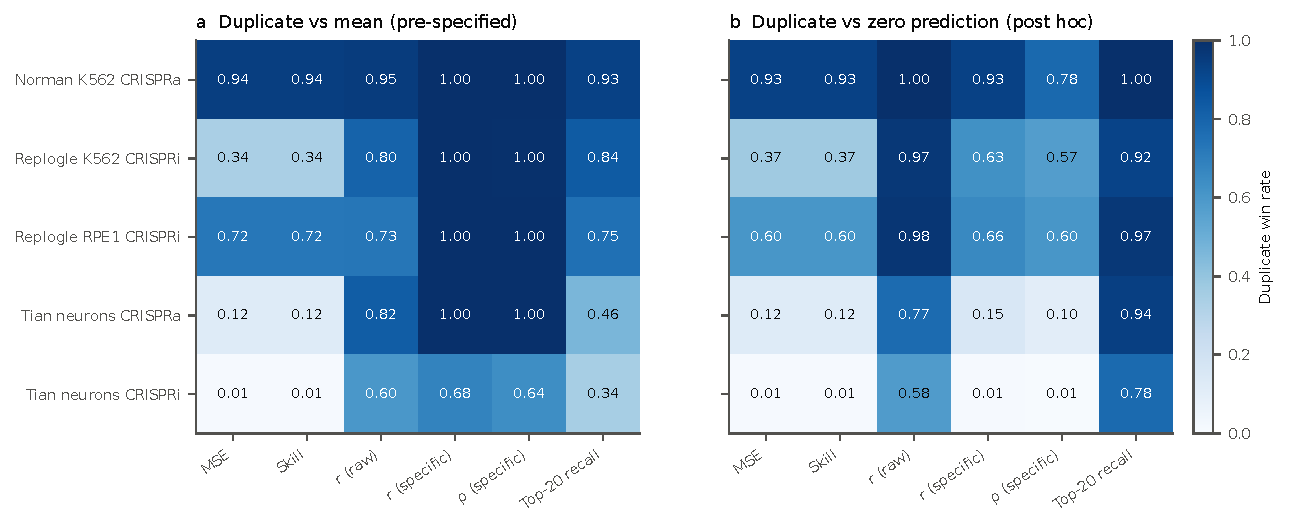
\includegraphics[width=\linewidth]{figures/fig6_calibration.pdf}
\caption{\textbf{Metric discrimination.} Fraction of single-gene perturbations for which a technical duplicate (the response from half of the cells and controls) scores better than an uninformative prediction of the other half. \textbf{a}, against the mean of other perturbations (pre-specified, addendum E4). \textbf{b}, against a zero prediction (post hoc). The two comparisons are separate; the better baseline is never chosen per perturbation. Undefined correlations of uninformative predictions count as 0. Wilson intervals are in Supplementary Table~\ref{tab:discrimination}.}
\label{fig:calibration}
\end{figure}

\subsection{Unseen genes: small but reproducible gains in large screens only}
The pre-specified confirmatory test C1 asked whether any learned model had lower MSE than the mean of training perturbations on held-out genes (Table~\ref{tab:c1}). The prediction of the discovery analysis, that none would, was \emph{refuted} in both Replogle screens: ridge regression, gene-loading ridge and the MLP ensemble all had lower MSE than the mean (all Holm-adjusted $p<0.001$; \numNCOneBeat{} of \numNCOneTests{} tests). The gains were small. Skill relative to the mean was \numSkillReplogleKEssentialMlpEnsemble{} (95\% CI \numSkillLoReplogleKEssentialMlpEnsemble--\numSkillHiReplogleKEssentialMlpEnsemble) for the MLP in K562 and \numSkillReplogleRpeMlpEnsemble{} (\numSkillLoReplogleRpeMlpEnsemble--\numSkillHiReplogleRpeMlpEnsemble) in RPE1, so the models removed about 5\% of the squared error left by the mean (Fig.~\ref{fig:unseen}a). The result was stable across three alternative fold partitions (Supplement). In the discovery dataset, no model was better than the mean (MLP skill \numSkillNormanMlpEnsemble, CI \numSkillLoNormanMlpEnsemble{} to \numSkillHiNormanMlpEnsemble). Norman is the screen where metrics discriminate best, so this is a genuine negative result rather than a measurement artefact.

In the neuron screens, no model met the pre-specified criterion, but one came close and the result needs care. In Tian CRISPRa, the MLP's signed-rank test was significant after Holm correction ($p_{\mathrm{Holm}}=0.0098$), but the bootstrap interval of its mean MSE difference included zero (Table~\ref{tab:c1}). The two parts of the rule disagree because the per-perturbation differences are skewed (Supplementary Fig.~\ref{fig:c1dist}). The MLP was better for \numTianAMlpFracBetter\% of perturbations, with a median difference of \numTianAMlpMedian{} ($\times10^{-3}$; 95\% CI \numTianAMlpMedianLo{} to \numTianAMlpMedianHi), but a few large losses brought the mean difference to \numTianAMlpMean. We therefore report that the MLP was typically, but not on average, better than the mean in this screen. The effect is small (skill \numSkillTianCrispraMlpEnsemble), in a screen where MSE has almost no power to discriminate, so we give it little weight in either direction. Beyond that, the C1 result in the neuron screens is uninformative rather than negative. With about 430 control cells, the training mean carries control-sampling noise that disjoint evaluation controls correctly fail to reward: predicting no change scored skill \numZeroSkillTianCrispra{} and \numZeroSkillTianCrispri{} relative to the mean.

Perturbation-specific correlations followed the same pattern (Fig.~\ref{fig:unseen}b). They reached \numSpecReplogleKEssentialMlpEnsemble{} (K562) and \numSpecReplogleRpeMlpEnsemble{} (RPE1) for the MLP, far below the technical reproducibility limits of \numCeilBatchReplogleKEssential{} and \numCeilBatchReplogleRpe. They were also only modestly above two controls: an MLP with permuted co-expression features (\numShufSpecReplogleKEssentialMlpEnsemble, \numShufSpecReplogleRpeMlpEnsemble), and the zero prediction (\numZeroSpecReplogleKEssential, \numZeroSpecReplogleRpe). Gains concentrated in perturbations whose responses are reproducible (post hoc). To avoid selecting on the outcome being scored, we selected perturbations using two cell halves within one set of batches, and scored the models against the response estimated from the other set, which shares no perturbed cells or batch-matched control cells with the selection. In K562, among the \numRiNReplogleKEssentialRidgeRep{} perturbations reproducible in the selection set, ridge reached skill \numRiSkillReplogleKEssentialRidgeRep{} (95\% CI \numRiLoReplogleKEssentialRidgeRep--\numRiHiReplogleKEssentialRidgeRep) and the MLP \numRiSkillReplogleKEssentialMlpEnsembleRep{} (\numRiLoReplogleKEssentialMlpEnsembleRep--\numRiHiReplogleKEssentialMlpEnsembleRep), against \numRiSkillReplogleKEssentialRidgeAll{} and \numRiSkillReplogleKEssentialMlpEnsembleAll{} over all perturbations scored the same way. In RPE1 (\numRiNReplogleRpeMlpEnsembleRep{} perturbations), the MLP reached \numRiSkillReplogleRpeMlpEnsembleRep{} (\numRiLoReplogleRpeMlpEnsembleRep--\numRiHiReplogleRpeMlpEnsembleRep). In Norman, nothing improved on the mean even among its \numRiNNormanRidgeRep{} reproducible perturbations (ridge \numRiSkillNormanRidgeRep, MLP \numRiSkillNormanMlpEnsembleRep). The neuron screens had too few reproducible perturbations (\numRiNTianCrispraRidgeRep{} and \numRiNTianCrispriRidgeRep) to assess.

\paragraph{Robustness (post hoc).} The Replogle results held under each sensitivity analysis (Supplementary Tables~\ref{tab:genesets}--\ref{tab:cellcount}):
\begin{itemize}
\item \emph{Output genes.} Scoring all detected genes rather than the 2{,}000 selected genes and targets gave MLP skill \numGsReplogleKEssentialMlpEnsembleExtended{} (K562) and \numGsReplogleRpeMlpEnsembleExtended{} (RPE1), and \numGsReplogleKEssentialMlpEnsembleOutsidePrimary{} and \numGsReplogleRpeMlpEnsembleOutsidePrimary{} on the genes outside the selected set. The harmonised Replogle files contain only genes expressed in the screen, so genes induced from silence can only be scored in Norman and the neuron screens, where no model beat the mean on them either.
\item \emph{Control-cell splits.} MLP skill ranged from \numCsMinReplogleKEssentialMlpEnsemble{} to \numCsMaxReplogleKEssentialMlpEnsemble{} (K562) and from \numCsMinReplogleRpeMlpEnsemble{} to \numCsMaxReplogleRpeMlpEnsemble{} (RPE1) across five independent control splits.
\item \emph{Initialisation.} MLP skill ranged from \numSeedMinReplogleKEssentialMlpEnsemble{} to \numSeedMaxReplogleKEssentialMlpEnsemble{} and from \numSeedMinReplogleRpeMlpEnsemble{} to \numSeedMaxReplogleRpeMlpEnsemble{} across five seeds.
\item \emph{Dependence between perturbations.} Targets share pathways and programmes, so we also resampled clusters of co-expressed targets rather than single perturbations (block bootstrap). Intervals for the primary C1 estimand, mean $\Delta$MSE, still excluded zero for all six Replogle tests. On mean skill, the MLP's intervals stayed above zero (K562 \numBlockLoReplogleKEssentialMlpEnsemble--\numBlockHiReplogleKEssentialMlpEnsemble; RPE1 \numBlockLoReplogleRpeMlpEnsemble--\numBlockHiReplogleRpeMlpEnsemble), but those of the linear models widened to include zero in RPE1 (ridge \numBlockLoReplogleRpeRidge--\numBlockHiReplogleRpeRidge).
\item \emph{Cell counts.} Skill was higher for perturbations measured in more cells (MLP in K562: \numCcFewestReplogleKEssentialMlpEnsemble{} in the third with fewest cells, \numCcMostReplogleKEssentialMlpEnsemble{} in the third with most), and excluding conditions with fewer than 100 cells raised it to \numCcHundredReplogleKEssentialMlpEnsemble{} (RPE1: \numCcHundredReplogleRpeMlpEnsemble).
\end{itemize}

\begin{table}[t]
\centering\scriptsize
\caption{Confirmatory test C1: learned models versus the mean baseline on held-out genes. $\Delta$MSE is the mean per-perturbation difference (model $-$ mean), multiplied by $10^3$; negative favours the model. $p$: one-sided Wilcoxon signed-rank; Holm correction across all 12 tests. ``Beats mean'' requires $p_{\mathrm{Holm}}<0.05$ and a 95\% bootstrap interval below 0.}
\label{tab:c1}
\resizebox{\linewidth}{!}{\begin{tabular}{llcrrrc}
\toprule
Dataset & Model & $\Delta$MSE$\times10^{3}$ vs mean (95\% CI) & Skill & $p$ & $p_{\mathrm{Holm}}$ & Beats mean \\
\midrule
Replogle K562 CRISPRi & Ridge & -0.231 (-0.280, -0.187) & 0.025 & $<$0.001 & $<$0.001 & yes \\
Replogle K562 CRISPRi & Gene-loading ridge & -0.214 (-0.267, -0.165) & 0.018 & $<$0.001 & $<$0.001 & yes \\
Replogle K562 CRISPRi & MLP ensemble & -0.274 (-0.331, -0.220) & 0.051 & $<$0.001 & $<$0.001 & yes \\
Replogle RPE1 CRISPRi & Ridge & -0.428 (-0.572, -0.296) & 0.011 & $<$0.001 & $<$0.001 & yes \\
Replogle RPE1 CRISPRi & Gene-loading ridge & -0.380 (-0.519, -0.251) & 0.010 & $<$0.001 & $<$0.001 & yes \\
Replogle RPE1 CRISPRi & MLP ensemble & -0.480 (-0.646, -0.324) & 0.052 & $<$0.001 & $<$0.001 & yes \\
Tian neurons CRISPRa & Ridge & +0.023 (+0.007, +0.043) & -0.010 & 0.99 & 1 & no \\
Tian neurons CRISPRa & Gene-loading ridge & +0.005 (+0.000, +0.011) & -0.001 & 0.96 & 1 & no \\
Tian neurons CRISPRa & MLP ensemble & -0.008 (-0.036, +0.023) & 0.012 & 0.0016 & 0.0098 & no \\
Tian neurons CRISPRi & Ridge & +0.000 (-0.000, +0.001) & -0.000 & 0.96 & 1 & no \\
Tian neurons CRISPRi & Gene-loading ridge & +0.000 (-0.000, +0.000) & -0.000 & 0.23 & 1 & no \\
Tian neurons CRISPRi & MLP ensemble & +0.001 (-0.001, +0.002) & -0.001 & 0.91 & 1 & no \\
\bottomrule
\end{tabular}}
\end{table}

\begin{figure}[t]
\centering
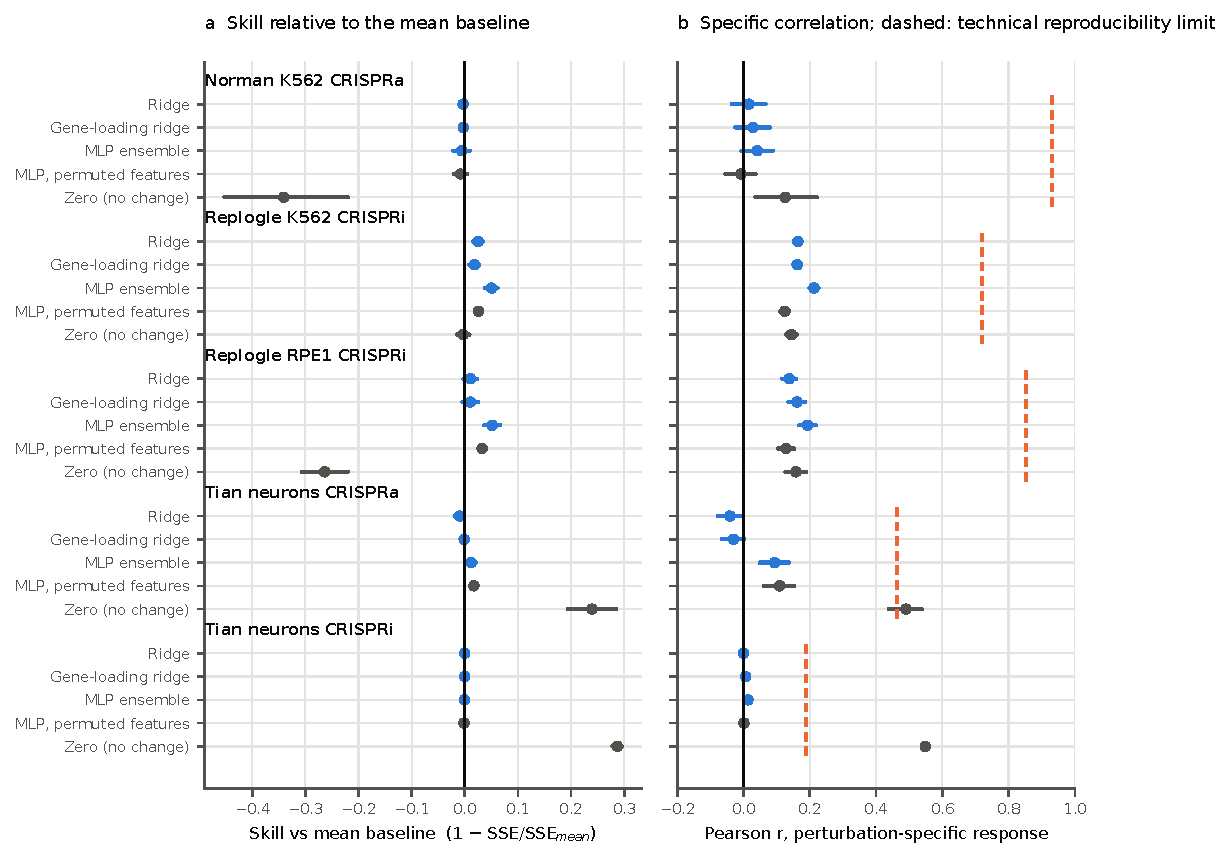
\includegraphics[width=\linewidth]{figures/fig2_unseen_genes.pdf}
\caption{\textbf{Prediction for genes absent from training.} Means over held-out perturbations with 95\% bootstrap intervals (5 folds, seed 0). Blue: pre-specified learned models with co-expression features. Grey: controls, namely the MLP with co-expression features permuted among genes (target baseline expression retained) and the zero prediction. \textbf{a}, skill relative to the training mean (0 = mean baseline). \textbf{b}, Pearson correlation of the perturbation-specific response, with the batch-disjoint technical reproducibility limit (dashed).}
\label{fig:unseen}
\end{figure}

\subsection{Co-expression features help in large screens; pretrained Gene2vec does not add to them}
Test C2 compared co-expression features with the same features permuted among genes; both kept the target's own control-cell expression. Co-expression improved skill for both ridge and the MLP in both Replogle screens (\numNCTwoInformative{} of \numNCTwoTests{} tests), but not in the neuron screens (Table~\ref{tab:c2c3}). The plan specified no multiplicity correction for C2. With a post-hoc Holm correction over its eight two-sided Wilcoxon tests, all four Replogle results remain significant (largest adjusted $p=\numCTwoMaxHolmReplogle$) and none of the neuron results are ($p_{\mathrm{Holm}}\ge\numCTwoMinHolmTian$). This shows that co-expression carries information about an unseen gene's response. It does not show that the information is practically useful: the gains are a few hundredths of skill (Table~\ref{tab:c2c3}). Test C3 asked whether frozen Gene2vec embeddings, trained on co-expression across 984 public datasets \citep{du2019gene2vec}, improve on co-expression from the screen's own control cells. They did not in general. Gene2vec was significantly \emph{worse} for ridge in K562. Only one of \numNCThreeTests{} tests favoured Gene2vec (MLP, Tian CRISPRi), by a skill difference of about 0.002, which is of no practical consequence. For the MLP in K562, the Holm-adjusted signed-rank test was significant ($p<0.001$) while the bootstrap interval of the mean skill difference included zero (\numCThreeMeanReplogleKEssentialMlpEnsemble). The cause is the same as in C1: the median difference was \numCThreeMedianReplogleKEssentialMlpEnsemble{} (95\% CI \numCThreeMedianLoReplogleKEssentialMlpEnsemble{} to \numCThreeMedianHiReplogleKEssentialMlpEnsemble), and Gene2vec was better for only \numCThreeFracReplogleKEssentialMlpEnsemble\% of perturbations. Gene2vec was thus typically slightly worse, but the average difference is uncertain. Mean and median estimates for every confirmatory test are in Supplementary Table~\ref{tab:estimands}.

\begin{table}[t]
\centering\scriptsize
\caption{Confirmatory tests C2 and C3 on held-out genes. Skill differences are per-perturbation paired means with 95\% bootstrap intervals. C2 is supported (co-expression informative) if the interval lies above 0. C3 uses a two-sided Wilcoxon test, Holm-corrected across its 8 tests.}
\label{tab:c2c3}
\resizebox{\linewidth}{!}{\begin{tabular}{lllllcc}
\toprule
Test & Contrast & Dataset & Model & Skill difference (95\% CI) & $p_{\mathrm{Holm}}$ & Supported \\
\midrule
C2 & Co-expression $-$ permuted & Replogle K562 CRISPRi & Ridge & +0.028 (+0.019, +0.035) & -- & yes \\
C2 & Co-expression $-$ permuted & Replogle K562 CRISPRi & MLP ensemble & +0.025 (+0.013, +0.035) & -- & yes \\
C2 & Co-expression $-$ permuted & Replogle RPE1 CRISPRi & Ridge & +0.018 (+0.005, +0.030) & -- & yes \\
C2 & Co-expression $-$ permuted & Replogle RPE1 CRISPRi & MLP ensemble & +0.019 (+0.005, +0.033) & -- & yes \\
C2 & Co-expression $-$ permuted & Tian neurons CRISPRa & Ridge & -0.009 (-0.017, -0.002) & -- & no \\
C2 & Co-expression $-$ permuted & Tian neurons CRISPRa & MLP ensemble & -0.005 (-0.010, +0.000) & -- & no \\
C2 & Co-expression $-$ permuted & Tian neurons CRISPRi & Ridge & +0.000 (-0.000, +0.001) & -- & no \\
C2 & Co-expression $-$ permuted & Tian neurons CRISPRi & MLP ensemble & +0.001 (-0.000, +0.002) & -- & no \\
C3 & Gene2vec $-$ co-expression & Replogle K562 CRISPRi & Ridge & -0.029 (-0.038, -0.019) & $<$0.001 & no \\
C3 & Gene2vec $-$ co-expression & Replogle K562 CRISPRi & MLP ensemble & -0.008 (-0.017, +0.004) & $<$0.001 & no \\
C3 & Gene2vec $-$ co-expression & Replogle RPE1 CRISPRi & Ridge & -0.008 (-0.023, +0.005) & 1 & no \\
C3 & Gene2vec $-$ co-expression & Replogle RPE1 CRISPRi & MLP ensemble & -0.004 (-0.017, +0.010) & 1 & no \\
C3 & Gene2vec $-$ co-expression & Tian neurons CRISPRa & Ridge & +0.008 (+0.001, +0.018) & 0.78 & no \\
C3 & Gene2vec $-$ co-expression & Tian neurons CRISPRa & MLP ensemble & -0.002 (-0.009, +0.006) & 1 & no \\
C3 & Gene2vec $-$ co-expression & Tian neurons CRISPRi & Ridge & +0.000 (-0.000, +0.000) & 1 & no \\
C3 & Gene2vec $-$ co-expression & Tian neurons CRISPRi & MLP ensemble & +0.002 (+0.000, +0.003) & 0.029 & yes \\
\bottomrule
\end{tabular}}
\end{table}

\subsection{What co-expression features carry (post hoc)}
To separate the components of the primary features, we refit ridge and the MLP on the primary folds with each component alone (Fig.~\ref{fig:ablation}; Supplementary Table~\ref{tab:ablation}). In both Replogle screens, co-expression alone matched the full feature set: MLP skill \numAblReplogleKEssentialMlpEnsembleCoexpressionOnly{} versus \numAblReplogleKEssentialMlpEnsembleFull{} in K562, and \numAblReplogleRpeMlpEnsembleCoexpressionOnly{} versus \numAblReplogleRpeMlpEnsembleFull{} in RPE1. The target's own control-cell expression level and detection rate behaved differently for the two models. With these two baseline features alone, the MLP reached about two-thirds of the full gain (\numAblReplogleKEssentialMlpEnsembleBaselineBoth{} and \numAblReplogleRpeMlpEnsembleBaselineBoth), whereas ridge reached almost none (\numAblReplogleKEssentialRidgeBaselineBoth{} and \numAblReplogleRpeRidgeBaselineBoth).

A large part of the usable signal is therefore available from how strongly and how broadly the target is expressed in unperturbed cells. The relation is not a simple monotonic one: target expression correlates only weakly with response magnitude (Spearman $\rho=0.16$ in K562 and $0.06$ in RPE1, post hoc), so the MLP's gain from these two features reflects nonlinear structure that our analyses do not resolve. The co-expression embedding largely subsumes this signal (adding the baseline features changed skill by at most 0.005) and adds a further component that a linear model can use. That component is consistent with broad transcriptional programmes shared by co-regulated genes, rather than with mechanism-specific information. These features are statistical associations measured in unperturbed cells, and our analyses do not show that they reflect causal regulatory relationships.

Because the control-derived features had used control cells from both random halves, including the half behind the evaluation targets, we recomputed them from the training half alone. Performance was unchanged: MLP skill \numAblReplogleKEssentialMlpEnsembleFullSplit{} (K562) and \numAblReplogleRpeMlpEnsembleFullSplit{} (RPE1), against \numAblReplogleKEssentialMlpEnsembleFull{} and \numAblReplogleRpeMlpEnsembleFull{} with the primary features. The results do not depend on that overlap.

\begin{figure}[t]
\centering
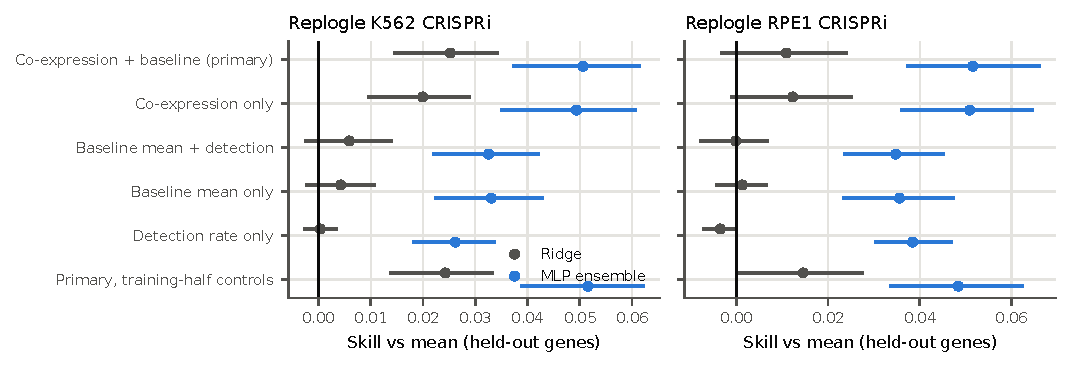
\includegraphics[width=0.95\linewidth]{figures/fig7_feature_ablation.pdf}
\caption{\textbf{Feature ablation in the large screens} (post hoc). Skill on held-out single genes with each feature component alone, and with the primary features recomputed from training-half control cells only. Means with 95\% bootstrap intervals; grey: ridge, blue: MLP ensemble.}
\label{fig:ablation}
\end{figure}

\subsection{Within a screen, gains grow with the number of training perturbations}
Subsampling training perturbations within fixed folds of the two Replogle screens (exploratory E1) showed a steady increase without a clear plateau (Fig.~\ref{fig:size}). Specific correlation rose from about 0.04 with 25 training perturbations to \numLcSpecFullReplogleKEssentialRidge{} (K562) and \numLcSpecFullReplogleRpeRidge{} (RPE1) with all of them, about 1{,}000, roughly linearly in the logarithm of training size. Skill rose too but remained small (ridge: \numLcFullReplogleKEssentialRidge{} and \numLcFullReplogleRpeRidge{}). With around 70 training perturbations, the size of the Norman training folds, skill in the Replogle screens is near zero and specific correlation below 0.1, consistent with the failure in the discovery screen. This is an association within one study's screens, from three draws per size. Screens also differ in modality, cell type, depth and number of controls, so the curves do not establish that training-set size is the main determinant of performance across experiments.

\begin{figure}[t]
\centering
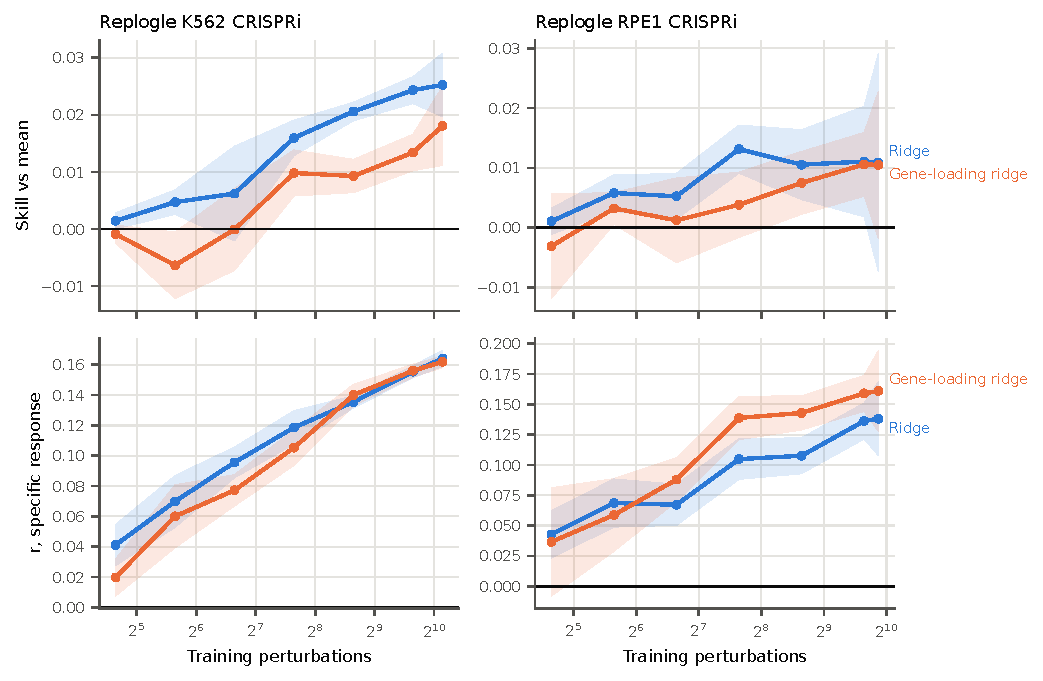
\includegraphics[width=0.92\linewidth]{figures/fig3_training_size.pdf}
\caption{\textbf{Performance against training-set size} (exploratory). Training perturbations subsampled within each fold (three draws per size), with test perturbations fixed. Means over folds and draws $\pm$1.96 standard errors.}
\label{fig:size}
\end{figure}

\subsection{A measurement in another cell line is about as informative as the best model}
For \numNSharedKToRpe{} genes knocked down in both Replogle screens (exploratory E2), the measured response in one cell line was a poor predictor in the other when used as is (skill \numCcTransferRawKToRpe{} for K562$\to$RPE1, \numCcTransferRawRpeToK{} for RPE1$\to$K562), because responses differ systematically in scale between the lines (Fig.~\ref{fig:cross}). Taking the source screen's specific response, rescaled by one factor fitted on other genes and added to the target screen's mean, gave skill \numCcTransferDeviationScaledKToRpe{} (\numCcLoTransferDeviationScaledKToRpe--\numCcHiTransferDeviationScaledKToRpe) and \numCcTransferDeviationScaledRpeToK{} (\numCcLoTransferDeviationScaledRpeToK--\numCcHiTransferDeviationScaledRpeToK), with specific correlation \numCcSpecTransferDeviationScaledKToRpe{} in both directions. That is comparable to the best unseen-gene model on the same targets. In this one pair of cell lines, a direct measurement of the same perturbation in the other line therefore carried about as much transferable gene-specific information as the models extract within the target screen. The two predictors use different information, a measurement elsewhere versus learned structure, and one rescaling factor is a simple transfer model, so this comparison is exploratory and may not hold for other pairs of contexts or modalities.

\begin{figure}[t]
\centering
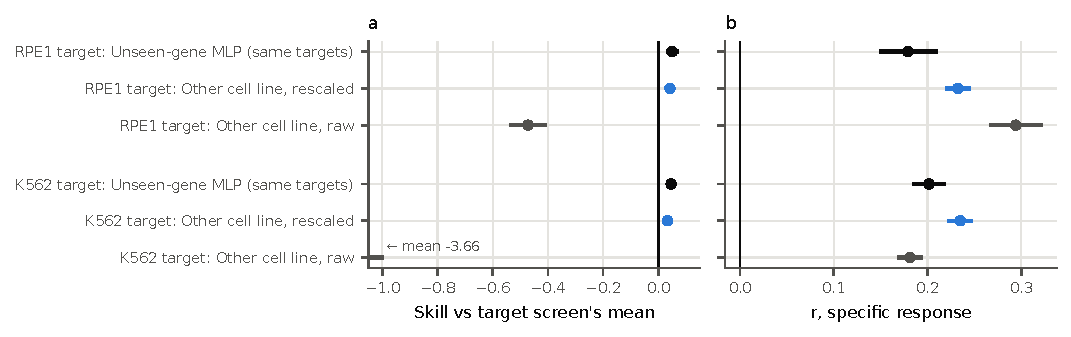
\includegraphics[width=0.95\linewidth]{figures/fig4_cross_context.pdf}
\caption{\textbf{Transfer between cell lines} (exploratory). Targets knocked down in both Replogle screens, scored on genes measured in both. ``Rescaled'': the target screen's mean plus the source screen's specific response, multiplied by one factor fitted on other targets. The unseen-gene MLP is shown on the same targets, scored on the target screen's full gene set.}
\label{fig:cross}
\end{figure}

\subsection{Ranking strong responders}
For prioritising experiments, the relevant question is whether the strongest responses can be found among untested genes (Supplementary Table~\ref{tab:ranking}). In K562, the top 20\% of held-out genes by predicted response magnitude contained \numRkReplogleKEssentialRidgeTwenty{} (ridge; 95\% CI \numRkLoReplogleKEssentialRidgeTwenty--\numRkHiReplogleKEssentialRidgeTwenty) of the truly strongest 20\%, against 0.20 expected by chance. In RPE1 the figure was \numRkReplogleRpeRidgeTwenty{} (\numRkLoReplogleRpeRidgeTwenty--\numRkHiReplogleRpeRidgeTwenty). Both were significant against random rankings at the 10\%, 20\% and 30\% thresholds (permutation $p<0.01$), and stable across MLP seeds (\numRkSeedMinReplogleKEssential--\numRkSeedMaxReplogleKEssential{} and \numRkSeedMinReplogleRpe--\numRkSeedMaxReplogleRpe{} at 20\%). In Norman and the neuron screens, rankings were not distinguishable from random. An enrichment of 1.5- to 3-fold, depending on screen and threshold, is statistically clear, but we have not shown that it would change experimental decisions; that requires prospective validation.

\subsection{Selected gene pairs: attenuated additive projection, captured by a single scale factor}
In the discovery screen, pairs whose single-gene responses were measured were predicted well by the sum of the singles (skill \numPairskillAdditive{} relative to the mean of pairs). A single global scale factor applied to that sum, fitted on training pairs, raised skill to \numPairskillScaledAdditive. Ridge and MLP models of the residual from the additive prediction reached \numPairskillRidgeOnAdditive{} and \numPairskillMlpOnAdditive, but their MSE was not distinguishable from the scaled sum (difference \numPairMseDiffScaled, 95\% CI \numPairMseDiffScaledLo{} to \numPairMseDiffScaledHi; Fig.~\ref{fig:pairs}b).

Because noise in the estimated single responses would bias a fitted scale factor towards zero, we estimated it per pair with an instrumental-variable estimator using independent halves of the single-perturbation cells. The median coefficient was \numBetaIvMedian{} (95\% CI \numBetaIvLo--\numBetaIvHi; least squares \numBetaOlsMedian), and \numFracBelowOne\% of the \numNPairs{} pairs were below 1 (Fig.~\ref{fig:pairs}a). The single responses were measured reliably (median split-half $r$ \numSinglesReliability), so the correction was small. For most of these pairs, the response projects less strongly onto the sum of the single responses than additivity would predict. A coefficient below 1 does not by itself establish biological sub-additivity. It is also consistent with weaker knockdown or activation by guides in the double-perturbation construct, with response components orthogonal to the additive direction, or with differences in cell state, survival or capture between single- and double-perturbation conditions. Moreover, the instrumental-variable correction assumes that the two halves of the single-gene cells measure the same response with independent errors. The pairs were chosen from a genetic-interaction map \citep{norman2019} and are enriched for interactions, and no other included screen contains pairs. We therefore report an attenuated additive projection among selected, interaction-enriched pairs, not a general property of combined perturbations.

\begin{figure}[t]
\centering
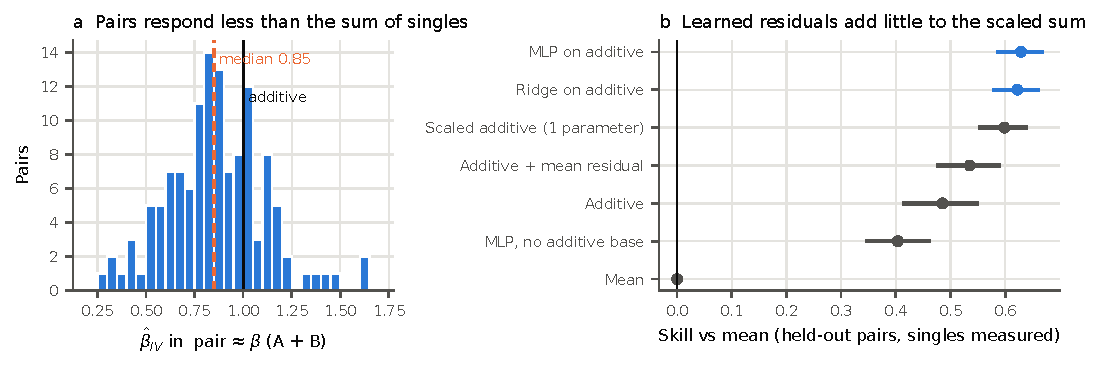
\includegraphics[width=\linewidth]{figures/fig5_pairs.pdf}
\caption{\textbf{Gene pairs in the discovery screen} (exploratory). \textbf{a}, per-pair coefficient $\beta$ in pair $\approx\beta\,$(A+B), estimated with an instrumental variable to remove attenuation from measurement error. \textbf{b}, skill on held-out pairs whose singles were measured; models in blue learn a residual from the additive prediction.}
\label{fig:pairs}
\end{figure}

\subsection{Prediction intervals}
Per-gene 90\% intervals calibrated on held-out residuals covered \numCovReplogleKEssential{} (K562), \numCovReplogleRpe{} (RPE1) and \numCovNorman{} (Norman) of genes overall. On each perturbation's 20 genes with the largest \emph{predicted} deviation from the mean, which is how genes would be chosen in practice, coverage was close to nominal: \numIvPredReplogleKEssentialMlpEnsemble{}, \numIvPredReplogleRpeMlpEnsemble{} and \numIvPredNormanMlpEnsemble{} for the MLP (Supplementary Table~\ref{tab:ivsel}). On the 20 genes with the largest \emph{observed} deviation, coverage fell to \numCovTopReplogleKEssential, \numCovTopReplogleRpe{} and \numCovTopNorman. That subset is selected on the outcome and preferentially contains large errors, so its low coverage does not show that the intervals are miscalibrated. It does show a practical limitation: the genes that turn out to respond most strongly are largely not the ones the models predict, so intervals are wide enough on average but rarely contain the extreme responses. Calibrating within strata of predicted magnitude did not change this (Supplementary Table~\ref{tab:intervals}).

\section{Discussion}
Across five Perturb-seq screens analysed under a fixed plan, transcriptional responses to genes absent from training were predictable only to a small extent by the models we evaluated, and only in the two large screens. There, models beat the mean of other perturbations reproducibly but removed about 5\% of its squared error. Their perturbation-specific correlations of about 0.2 compare with technical reproducibility limits of 0.72--0.85. In the discovery screen, whose metrics are well calibrated and whose responses are highly reproducible, no model improved on the mean at all. The difference tracks the number of training perturbations, and performance in the large screens rose steadily with it. Among gene pairs selected for interactions, responses were well described by a scaled sum of the single responses, and learned models of the remainder were not distinguishable from that one-parameter rule.

\paragraph{Scope of the conclusions.} Our model set was deliberately simple: linear and nearest-neighbour baselines and small neural-network ensembles, using co-expression, target baseline expression or Gene2vec features. We did not evaluate graph neural networks such as GEARS \citep{roohani2024} or pretrained single-cell foundation models \citep{cui2024}. The results show how much predictive information these representations carry with these model classes, which is what limits the models tested here. They do not show that Perturb-seq data are fundamentally insufficient for stronger models, and they do not rank the field's methods. The protocol, however, applies to any model, and the reproducibility limits and calibration checks do not depend on the model at all.

\paragraph{Relation to the baseline debate.} The results bear on whether deep models beat simple baselines \citep{ahlmanneltze2025,csendes2025,vinastorne2025,miller2026}. We confirm the core of \citet{miller2026}'s argument: MSE was poorly calibrated in four of five screens, ranking half-data replicates below the mean for most perturbations. We also extend the observation of \citet{csendes2025} that common benchmarks have low perturbation-specific variance. With batch-disjoint replicates, between a quarter and two-thirds of perturbations in the large CRISPRi screens, and almost all in the neuron screens, have specific responses that do not reproduce. Remedies depend on the reference, though. Perturbation-specific correlation looks perfectly calibrated against the mean, yet a zero prediction scores well on it whenever perturbations vary mostly in magnitude, or whenever the training mean is dominated by control-sampling noise. Once noise is quantified and more than one uninformative control is used, the answer for the models tested is neither ``learned models fail'' nor ``learned models succeed''. They extract a real but small signal when training sets are large.

\paragraph{What the models learn.} The feature ablation helps interpret that signal. Much of it is available to a nonlinear model from the target's own expression level and detection rate in unperturbed cells. These are generic properties of the gene, and they relate to response magnitude only weakly and non-monotonically. Signal of this kind can help rank perturbations, but it says little about which downstream genes change. Co-expression across control cells adds a component that even a linear model can use, consistent with broad co-regulated programmes in which genes that vary together at baseline also share responses to perturbation. Two observations argue that this signal is generic rather than mechanistic: specific correlations stay far below the technical limits, and a measured response of the same gene in another cell line was only about as informative as the models. Most of a perturbation's specific transcriptional response therefore appears to depend on cellular context and is not recoverable from these representations. Generic pretrained embeddings did not close the gap: Gene2vec, built from co-expression across 984 datasets, did not beat co-expression measured in each screen's own control cells.

\paragraph{Implications for prioritising experiments.} The practical value is correspondingly limited, with three qualifications. First, in the large screens model rankings found strong responders at about 1.7 times the chance rate, a modest but usable gain. Second, for pairs whose singles are measured, nearly all of the predictable signal comes from the singles, so a scaled sum is a strong, transparent default. Third, and most important for practice, prediction intervals were reliable on average but covered only 35--55\% of the most strongly responding genes. Stratifying calibration by predicted magnitude did not fix this, because the models do not anticipate which genes will respond. Uncertainty estimates for the genes that matter most should not be relied on with these models.

\paragraph{Methodological lessons.} Several points generalise. Training and evaluation targets should not share control cells. With few controls, a shared control population couples every response to the same noise and changes which baseline looks best: the training mean was worse than predicting no change in both neuron screens. Reproducibility limits should come from disjoint batches and be labelled as technical limits. Here the batch-disjoint and split-cell limits agreed closely except in the Tian CRISPRa screen, where the batch-disjoint limit was lower (\numCeilBatchTianCrispra{} versus \numCeilHalfTianCrispra). Metric calibration should be checked against more than one uninformative prediction. Composite decision rules should report both of their components: a model can be better for most perturbations yet not on average. Finally, conclusions drawn from a single dataset can be wrong in either direction. The discovery screen suggested that no model beats the mean, and in larger screens that conclusion was refuted, if only modestly.

\paragraph{Limitations.} The study covers five screens from two laboratories. Two candidate screens were excluded for label problems in the harmonised files that study-specific curation could have resolved. Genome-wide screens and other modalities were not analysed. Batches are technical lanes within each experiment, so the reproducibility limits omit biological replicate variation, such as independent cultures or repeated experiments. Our results therefore describe predictability within an experiment, and performance against an independent repeat of a screen would be lower. The pair analysis rests on one screen whose pairs were selected for interactions. All discovery-set baselines and metrics were defined after seeing discovery data. Several analyses were defined after seeing confirmation data, including the zero-prediction calibration control, the reproducible-subset sensitivity analysis, the feature ablation and the stratified intervals; these are labelled post hoc throughout. The analysis plan was not registered with a third party.

\section{Methods}

\subsection{Study design and analysis plan}
Norman et al.\ 2019 \citep{norman2019} served as the discovery dataset: all modelling and evaluation choices were developed on it, and several baselines and metrics were added after first results on its folds (disclosed in the Supplement). Before any other dataset was preprocessed or analysed, an analysis plan was written that fixed the datasets, inclusion rules, preprocessing, splits, models, hyperparameter grids, confirmatory tests and multiple-testing correction (\texttt{docs/analysis\_plan.md}; full SHA-256 in Supplementary Table~\ref{tab:hashes}). One addendum, adding a metric-calibration analysis motivated by \citet{miller2026}, was written before any confirmation dataset was analysed (\texttt{docs/analysis\_plan\_addendum.md}). Both hashes are verified and recorded by the study runner. The plan and addendum were not registered with a third party, so their timing rests on the project's own records.

\subsection{Data}
All data were the harmonised H5AD files of scPerturb \citep{peidli2024}, Zenodo record 13350497 (version 1.4, CC-BY-4.0), each verified against its published MD5 checksum. Candidate confirmation datasets were Replogle et al.\ 2022 K562 essential-gene and RPE1 CRISPRi screens \citep{replogle2022}, the Adamson et al.\ 2016 unfolded-protein-response CRISPRi screen \citep{adamson2016}, the Dixit et al.\ 2016 day-7 K562 knockout screen \citep{dixit2016}, and the Tian et al.\ 2021 iPSC-derived neuron CRISPRa and CRISPRi screens \citep{tian2021}.

\paragraph{Inclusion.} A dataset was included if it passed checksum and schema validation; had at least 100 cells labelled \texttt{control} in the harmonised \texttt{perturbation} column; had at least 30 single-gene conditions with at least 50 cells (25 if fewer than 30 qualified at 50); and at least 80\% of its target labels resolved to a measured gene, directly or via HGNC-to-Ensembl mapping. Control groups were never inferred from guide names. Conditions with more than one target were excluded from the confirmation study.

\subsection{Preprocessing and response targets}
Where present, cells were restricted to \texttt{good\_coverage} and \texttt{number\_of\_cells}$=1$. Counts were scaled to $10^4$ per cell over all genes and log1p-transformed. Statistics were accumulated in chunks along the matrix's storage axis, so peak memory stayed below 2\,GB for the largest dataset (310{,}385 cells). Genes were selected using control cells only. Among genes detected in at least 1\% of control cells, dispersion was computed as the variance divided by the mean of log-normalised expression. Genes were divided into 20 quantile bins of mean expression, dispersion was $z$-scored within each bin, and the 2{,}000 genes with the highest $z$-scores were kept. All target genes were then added.

For condition $p$, gene $g$ and batch $r$ (10x lane), with $w_{pr}$ the fraction of $p$'s cells in batch $r$, the response is
\begin{equation}
\Delta_{pg} \;=\; \sum_r w_{pr}\big(\bar x_{pgr} - \bar c_{gr}\big) \;=\; \bar x_{pg} - \sum_r w_{pr}\,\bar c_{gr},
\end{equation}
where $\bar x$ and $\bar c$ are mean log-normalised expression in perturbed and control cells. The second form avoids storing per-condition-per-batch statistics. Control cells were split at random into two halves within each batch. Training targets $\Delta^{\mathrm{fit}}$ use one half and evaluation targets $\Delta^{\mathrm{eval}}$ the other, so no control noise is shared between the two. The perturbed gene's own entry is masked in its own condition, both in training and in all metrics, because CRISPRa and CRISPRi alter their targets directly.

\subsection{Splits}
In the \emph{unseen-gene} task, target genes are partitioned into five folds. Every condition containing a held-out gene is removed from training and tested. A calibration set is built the same way from 15\% of the remaining genes and used for hyperparameter selection, early stopping and interval calibration. An automated check rejects any fold in which a held-out or calibration gene, or a duplicated gene set, appears in training. In Norman, the \emph{unseen-pair} task holds out pairs whose two single-gene responses are in training.

\subsection{Models}
\textbf{Mean}: the mean training response (per number of targets). \textbf{Ridge}: ridge regression on the residual from the mean, using a perturbation representation. \textbf{Gene-loading ridge}: following \citet{ahlmanneltze2025}, the target is represented by its loadings in a PCA of the training response matrix. \textbf{kNN}: average residual of the nearest training perturbations. \textbf{MLP ensemble}: five bootstrap-trained networks (two hidden layers, 128 and 64 units, dropout 0.1, Huber loss, AdamW, early stopping), predicting 20 principal components of training residuals. \textbf{Additive}, \textbf{scaled additive} (one global factor fitted on training pairs) and \textbf{additive plus mean residual} were used for pairs, together with ridge and MLP variants that learn the residual from the additive prediction.

A perturbation representation is the sum of its targets' gene vectors, plus the targets' control expression and detection rate. Gene vectors were of three kinds. The first was a 32-dimensional co-expression embedding. Log-normalised expression of the selected genes in at most 8{,}000 randomly sampled control cells was centred and scaled to unit variance per gene; genes with zero variance were set to 0. The resulting matrix was decomposed by randomised truncated SVD (seed 0), and each gene's vector is its row of the right singular vectors, multiplied by the singular values and divided by $\sqrt{n_{\text{cells}}}$. The target's own baseline features are its mean log-normalised expression and its detection rate (fraction of cells with nonzero counts) over all control cells. These features use control cells from both random halves, including the half behind the evaluation targets; a post-hoc check recomputed them from the training half alone (Supplement). The second kind of gene vector was the same embedding with rows randomly permuted among genes, as a negative control. Permutation leaves each target's baseline features unchanged, so this control isolates the contribution of co-expression. The third kind was frozen 200-dimensional Gene2vec embeddings \citep{du2019gene2vec}. Perturbation features were standardised using training conditions only within each fold. Full hyperparameter grids and seeds are in Supplementary Table~\ref{tab:grids}. In the discovery dataset, STRING-derived features \citep{szklarczyk2023} were also examined (Supplement).

\subsection{Metrics}
For each held-out perturbation, excluding masked entries: mean squared error (MSE); \emph{skill} $=1-\mathrm{SSE}_{\text{model}}/\mathrm{SSE}_{\text{mean}}$; Pearson correlation of the raw response; and the Pearson and Spearman correlation of the \emph{perturbation-specific} response, the deviation from the training mean \citep[cf.\ the perturbed-centroid reference of][]{vinastorne2025}. The mean baseline has skill 0 by definition and no defined specific correlation. Perturbations are the unit of inference. Intervals are 95\% percentile bootstraps over perturbations (2{,}000 resamples), and paired comparisons use per-perturbation differences.

\paragraph{Technical reproducibility limits.} Each response was re-estimated from two disjoint sets of batches (alternating lanes), each against its own batch-matched controls. The correlation $r$ between the two estimates of the perturbation-specific response gives a Spearman--Brown \citep{spearman1910,brown1910} reliability $2r/(1+r)$ for the full estimate. Its square root approximates the correlation that a noiseless prediction of the expected response \emph{in this experiment} could reach. This rests on three assumptions: the two halves estimate the same expected response with independent errors; the errors have equal variance; and averaging the halves doubles the effective sample. Because the batches are technical lanes within one experiment, the limit captures sampling and lane-to-lane technical noise, but not variation between independent biological replicates, cultures or days. We therefore call it a \emph{technical} reproducibility limit; against an independently repeated experiment, the attainable correlation would be lower.

\paragraph{Metric calibration.} Following the logic of \citet{miller2026}, each metric was scored for a positive control (a technical duplicate: the response from one random half of a condition's cells and controls, predicting the other half) and a negative control (the mean of other conditions). A metric was called calibrated on a dataset if the duplicate won for at least 80\% of conditions.

\subsection{Confirmatory tests}
\textbf{C1:} For each confirmation dataset and pre-specified learned model (ridge, gene-loading ridge, MLP ensemble; co-expression features), a one-sided Wilcoxon signed-rank test of lower per-perturbation MSE than the mean baseline, with Holm correction \citep{holm1979} across all dataset--model tests. A model beats the mean if its adjusted $p<0.05$ \emph{and} the bootstrap interval of the mean MSE difference lies below 0. The two parts test different things. The signed-rank test concerns the location of the per-perturbation differences (whether the model is typically better), and the bootstrap interval concerns the average effect (whether expected error is lower). Requiring both guards against declaring an improvement when most perturbations improve slightly but a few deteriorate enough to raise average error, which matters for a tool whose errors are paid per experiment. \textbf{C2:} co-expression versus permuted co-expression; informative if the 95\% interval of the paired skill difference lies above 0. The plan applied no multiplicity correction to C2. A Holm-corrected two-sided Wilcoxon version is reported as a post-hoc sensitivity analysis. \textbf{C3:} Gene2vec versus co-expression, two-sided Wilcoxon with Holm correction.

\subsection{Exploratory analyses}
\textbf{Training-set size} (Replogle screens): training conditions were subsampled to 25--800 (three draws per size) within fixed folds. \textbf{Cross-context transfer}: for targets measured in both Replogle screens, on shared genes, one cell line's measured response predicted the other's, either raw or as the target dataset's mean plus a rescaled deviation (scale fitted on other targets). \textbf{Pair coefficients} (Norman): for each pair, $\beta$ in $\Delta_{\text{pair}}\approx\beta(\Delta_A+\Delta_B)$, estimated by least squares and by an instrumental-variable estimator, $\hat\beta_{\text{IV}}=\langle s^{(1)},y\rangle/\langle s^{(1)},s^{(2)}\rangle$. Here $s^{(1)},s^{(2)}$ are the summed single responses from disjoint halves of the single-perturbation cells, which removes attenuation from measurement error in the singles.

\subsection{Post-hoc analyses added in revision}
All of the following were added after the confirmatory results were seen. The first was a feature ablation, which refit ridge and the MLP on the primary folds with co-expression only, baseline mean only, detection rate only, both baseline features, and the primary features recomputed from training-half control cells. The second was a magnitude-stratified interval calibration, in which the interval quantile is calibrated separately within five strata of predicted deviation from the training mean, ranked within each perturbation. The strata are therefore defined from predictions alone and are available at prediction time. The third analysed the distribution of per-perturbation MSE differences behind C1.

\subsection{Software and reproducibility}
The pipeline is a Python package (Python 3.11.15, PyTorch 2.14.1, scikit-learn 1.9.1, NumPy 2.4.6, SciPy 1.17.1, pandas 2.3.3, AnnData 0.12.19; exact versions in \texttt{requirements-lock.txt}) with 149 automated tests, run on a laptop CPU (Apple M3, 8\,GB). Two complete runs of the discovery benchmark gave identical per-perturbation metrics. Every run records its configuration, split assignments, data checksums, target digests, package versions and the analysis-plan hashes.

\section*{Data and code availability}
All data are public and were obtained from scPerturb \citep{peidli2024} (Zenodo record 13350497, version 1.4); MD5 checksums and retrieval dates for every file are in the repository. The code, configuration files, analysis plan and addendum, exact package versions (\texttt{requirements-lock.txt}), fixed seeds, and the scripts that download and preprocess the data and generate every figure, table and quoted number are at \url{https://github.com/NaMEleSs0616/perturbation-response}. AUTHOR-TO-CONFIRM: the repository is currently private and will be made public, with a tagged release identified by its commit hash, before submission. SHA-256 hashes of the analysis plan, addendum and configuration files are listed in Supplementary Table~\ref{tab:hashes}. The confirmatory study is reproduced by \texttt{python -m biophysical.cli study run -{}-config configs/study.yaml}, and the post-hoc analyses by the scripts in \texttt{paper/scripts/}.

\section*{Use of AI assistance}
AUTHOR-TO-CONFIRM: The software, analyses and an initial draft of this manuscript were produced with the assistance of an AI coding assistant (Claude, Anthropic) under the author's direction. The author is responsible for the content.

\section*{Competing interests}
None declared.

\bibliographystyle{unsrtnat}
\bibliography{refs}
\clearpage
\appendix
\section*{Supplementary information}
\renewcommand{\thetable}{S\arabic{table}}
\renewcommand{\thefigure}{S\arabic{figure}}
\setcounter{table}{0}
\setcounter{figure}{0}

\subsection*{S1. File identities}
\begin{table}[H]
\centering\scriptsize
\caption{SHA-256 hashes of the files that fix the analysis. The study runner recomputes the plan and addendum hashes at launch and records them in \texttt{results/study/primary/study.json}; both matched. Hashes of downloaded data files (MD5, as published by Zenodo) are in \texttt{docs/data\_sources.md} and each dataset's \texttt{download.json}.}
\label{tab:hashes}
\begin{tabular}{ll}
\toprule
File & SHA-256 \\
\midrule
\texttt{docs/analysis\_plan.md} & \texttt{602693ec8bead09526c51498a22588a5ab3cc24ceaf9943b402b4f55bad273cc} \\
\texttt{docs/analysis\_plan\_addendum.md} & \texttt{48d36c4965da3155e3adb6fdfd14c2a83eaee64ba518643aaccbe4307bfce054} \\
\texttt{configs/study.yaml} & \texttt{b762a26d9610a8c88d5111a48807447a24110402fbe3d519e10d09e99c51b71c} \\
\texttt{configs/benchmark\_norman.yaml} & \texttt{4ebdd9199f9d4d4216da69b0cd7aa32b94d27f13d8edaf916d9e93603321e618} \\
\texttt{requirements-lock.txt} & \texttt{a5336ce52ab9b2cb11d251805b47eb7801917db72a41e67cf0bd08c3b73a3944} \\
\bottomrule
\end{tabular}
\end{table}

\subsection*{S2. Hyperparameters and seeds}
\begin{table}[H]
\centering\scriptsize
\caption{Settings used in every dataset (from \texttt{configs/benchmark\_norman.yaml} and \texttt{configs/study.yaml}). Hyperparameters marked ``selected'' were chosen per fold on the calibration genes by masked MSE.}
\label{tab:grids}
\begin{tabularx}{\linewidth}{lX}
\toprule
Component & Setting \\
\midrule
Preprocessing & $10^4$ counts per cell, log1p; 2{,}000 genes by binned dispersion in control cells (20 bins, detection $\ge1\%$) plus targets; $\ge50$ cells per condition (25 fallback); co-expression embedding 32 dimensions from $\le$8{,}000 control cells \\
Splits & 5 folds over target genes, fold seed 0 (robustness seeds 1--3); 15\% of remaining genes for calibration \\
Ridge & $\alpha\in\{0.1,1,10,100,1000,10000\}$, selected; features standardised on training conditions \\
Gene-loading ridge & 10 principal components of the training residual matrix; $\alpha$ as ridge, selected \\
kNN & $k\in\{1,3,5,10\}$, selected; neighbours among conditions with the same number of targets \\
Bootstrap ridge & 8 bootstrap members; $\alpha$ selected as ridge \\
MLP ensemble & 5 members, each on a bootstrap resample, member seed $1000m$; hidden layers 128 and 64 (ReLU), dropout 0.1; output 20 PCA components of training residuals; Huber loss ($\delta=1$); AdamW, learning rate $10^{-3}$, weight decay $10^{-3}$, batch 32; at most 400 epochs, early stopping with patience 40 on calibration loss \\
Intervals & 90\% per-gene, split-conformal style on calibration-gene residuals; per-gene scale = median absolute residual, floored at 10\% of the median scale \\
Ranking & top 20\% of held-out perturbations by predicted RMS response \\
\bottomrule
\end{tabularx}
\end{table}

\subsection*{S3. Discovery benchmark on Norman 2019}
The discovery benchmark trained on single genes and pairs together and evaluated three held-out strata in the unseen-gene task, plus pairs whose singles were measured (Table~\ref{tab:discovery}). These analyses informed the models, baselines and metrics in the analysis plan. Scaled additive, additive plus mean residual, singles-only models, the non-additive and top-gene coverage metrics, and the pair-ranking analyses were all added after first results on these same folds. Their discovery estimates are therefore optimistic in an unknown direction and are not confirmatory.

\begin{table}[H]
\centering\scriptsize
\caption{Discovery benchmark (Norman 2019; 5 folds, seed 0). Models trained with pairs and singles. Skill is relative to the training mean; $r$, specific is the correlation of deviations from it. In the confirmation study, models were trained on single-gene conditions only, which changes the unseen-single results (main text).}
\label{tab:discovery}
\begin{tabular}{llccr}
\toprule
Stratum & Model & Skill vs mean (95\% CI) & $r$, specific & $n$ \\
\midrule
Pair, both singles measured & mlp\_on\_additive & 0.629 (0.588, 0.666) & 0.832 & 127 \\
 & ridge\_on\_additive & 0.622 (0.581, 0.660) & 0.828 & 127 \\
 & bootstrap\_ridge\_on\_additive & 0.615 (0.572, 0.653) & 0.825 & 127 \\
 & scaled\_additive & 0.598 (0.555, 0.638) & 0.790 & 127 \\
 & knn\_on\_additive & 0.597 (0.539, 0.648) & 0.822 & 127 \\
 & additive\_plus\_mean\_residual & 0.535 (0.478, 0.589) & 0.810 & 127 \\
 & additive & 0.485 (0.415, 0.548) & 0.796 & 127 \\
 & mlp\_ensemble & 0.404 (0.348, 0.460) & 0.655 & 127 \\
 & ridge & 0.222 (0.147, 0.289) & 0.516 & 127 \\
 & knn & 0.182 (0.097, 0.261) & 0.487 & 127 \\
 & bootstrap\_ridge & 0.181 (0.095, 0.261) & 0.498 & 127 \\
 & gene\_loading\_ridge & 0.078 (0.038, 0.116) & 0.260 & 127 \\
 & ridge\_singles\_only & 0.055 (-0.012, 0.116) & 0.319 & 127 \\
 & mean & 0.000 (0.000, 0.000) & -- & 127 \\
 & gene\_loading\_singles\_only & -0.079 (-0.132, -0.029) & 0.080 & 127 \\
Pair, one gene unseen & mlp\_ensemble & 0.071 (0.033, 0.108) & 0.309 & 100 \\
 & ridge & 0.051 (0.018, 0.082) & 0.291 & 100 \\
 & bootstrap\_ridge & 0.042 (0.011, 0.073) & 0.268 & 100 \\
 & gene\_loading\_ridge & 0.004 (-0.018, 0.022) & 0.127 & 100 \\
 & mean & 0.000 (0.000, 0.000) & -- & 100 \\
 & ridge\_singles\_only & -0.008 (-0.064, 0.044) & 0.175 & 100 \\
 & gene\_loading\_singles\_only & -0.017 (-0.075, 0.037) & 0.165 & 100 \\
 & knn & -0.031 (-0.101, 0.040) & 0.240 & 100 \\
Unseen single gene & mean & 0.000 (0.000, 0.000) & -- & 105 \\
 & gene\_loading\_singles\_only & -0.003 (-0.007, 0.001) & 0.028 & 105 \\
 & ridge\_singles\_only & -0.003 (-0.010, 0.003) & 0.016 & 105 \\
 & gene\_loading\_ridge & -0.018 (-0.037, -0.003) & 0.022 & 105 \\
 & ridge & -0.124 (-0.234, -0.038) & 0.051 & 105 \\
 & bootstrap\_ridge & -0.127 (-0.226, -0.046) & 0.024 & 105 \\
 & mlp\_ensemble & -0.175 (-0.306, -0.062) & 0.062 & 105 \\
 & knn & -0.288 (-0.372, -0.202) & -0.029 & 105 \\
\bottomrule
\end{tabular}
\end{table}

\subsection*{S4. Robustness to the fold partition}
Pre-specified analysis D4 repeated the unseen-gene task with three further fold partitions (Table~\ref{tab:seeds}).

\begin{table}[H]
\centering\scriptsize
\caption{Mean skill relative to the training mean on held-out genes, for four fold partitions. Seed 0 is the primary analysis.}
\label{tab:seeds}
\begin{tabular}{llrrrr}
\toprule
Dataset & Model & Seed 0 & Seed 1 & Seed 2 & Seed 3 \\
\midrule
Norman K562 CRISPRa & Gene-loading ridge & -0.003 & -0.009 & -0.007 & -0.001 \\
Norman K562 CRISPRa & MLP ensemble & -0.006 & -0.012 & -0.013 & -0.003 \\
Norman K562 CRISPRa & Ridge & -0.003 & -0.006 & -0.001 & -0.001 \\
Replogle K562 CRISPRi & Gene-loading ridge & 0.018 & 0.008 & 0.014 & 0.012 \\
Replogle K562 CRISPRi & MLP ensemble & 0.051 & 0.045 & 0.051 & 0.050 \\
Replogle K562 CRISPRi & Ridge & 0.025 & 0.024 & 0.020 & 0.026 \\
Replogle RPE1 CRISPRi & Gene-loading ridge & 0.010 & 0.004 & 0.006 & 0.008 \\
Replogle RPE1 CRISPRi & MLP ensemble & 0.052 & 0.046 & 0.052 & 0.061 \\
Replogle RPE1 CRISPRi & Ridge & 0.011 & 0.002 & 0.008 & 0.010 \\
Tian neurons CRISPRa & Gene-loading ridge & -0.001 & -0.009 & -0.028 & -0.000 \\
Tian neurons CRISPRa & MLP ensemble & 0.012 & 0.007 & 0.009 & 0.017 \\
Tian neurons CRISPRa & Ridge & -0.010 & -0.008 & -0.001 & 0.001 \\
Tian neurons CRISPRi & Gene-loading ridge & -0.000 & -0.000 & -0.000 & 0.000 \\
Tian neurons CRISPRi & MLP ensemble & -0.001 & -0.001 & -0.000 & -0.000 \\
Tian neurons CRISPRi & Ridge & -0.000 & -0.000 & -0.000 & -0.000 \\
\bottomrule
\end{tabular}
\end{table}

\subsection*{S5. Distribution of per-perturbation differences behind C1 (post hoc)}
Figure~\ref{fig:c1dist} and Table~\ref{tab:c1med} show the full distribution of per-perturbation MSE differences, with the median alongside the mean. In the Replogle screens the median difference favours every model and the distributions are left-skewed: a minority of perturbations is predicted much better than by the mean. In Tian CRISPRa, the MLP is better for most perturbations, but a few large right-tail losses move the mean towards zero (main text).

\begin{figure}[H]
\centering
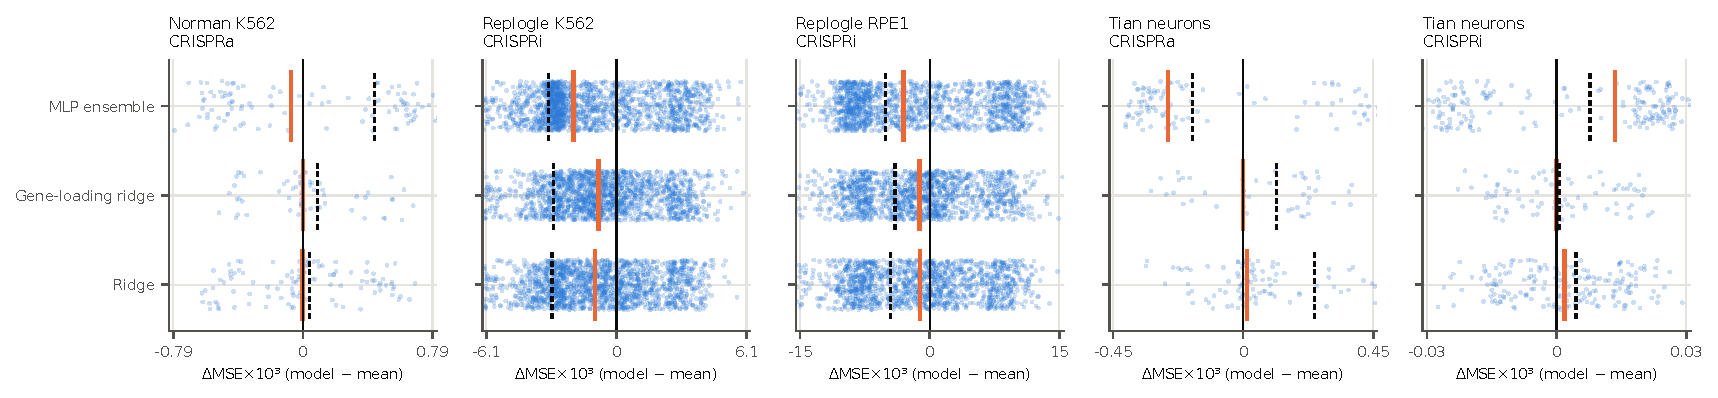
\includegraphics[width=\linewidth]{figures/figS1_c1_distribution.pdf}
\caption{Per-perturbation difference in MSE between each model and the mean baseline (negative favours the model), on a symmetric-log axis. Each point is one held-out gene. Orange: median; dashed black: mean.}
\label{fig:c1dist}
\end{figure}

\begin{table}[H]
\centering\scriptsize
\caption{Mean and median per-perturbation $\Delta$MSE $\times10^3$ (model $-$ mean), with bootstrap 95\% intervals for the median, and the fraction of perturbations on which the model is better.}
\label{tab:c1med}
\resizebox{0.9\linewidth}{!}{\begin{tabular}{llrcr}
\toprule
Dataset & Model & Mean $\Delta$MSE$\times10^3$ & Median (95\% CI) & Model better \\
\midrule
Norman K562 CRISPRa & Ridge & +0.004 & -0.000 (-0.005, +0.006) & 51\% \\
Norman K562 CRISPRa & Gene-loading ridge & +0.008 & -0.000 (-0.000, +0.000) & 50\% \\
Norman K562 CRISPRa & MLP ensemble & +0.061 & -0.007 (-0.031, +0.041) & 51\% \\
Replogle K562 CRISPRi & Ridge & -0.231 & -0.050 (-0.059, -0.039) & 62\% \\
Replogle K562 CRISPRi & Gene-loading ridge & -0.214 & -0.042 (-0.047, -0.037) & 64\% \\
Replogle K562 CRISPRi & MLP ensemble & -0.274 & -0.101 (-0.109, -0.088) & 67\% \\
Replogle RPE1 CRISPRi & Ridge & -0.428 & -0.105 (-0.141, -0.046) & 56\% \\
Replogle RPE1 CRISPRi & Gene-loading ridge & -0.380 & -0.110 (-0.150, -0.075) & 59\% \\
Replogle RPE1 CRISPRi & MLP ensemble & -0.480 & -0.284 (-0.366, -0.199) & 60\% \\
Tian neurons CRISPRa & Ridge & +0.023 & +0.001 (+0.000, +0.002) & 38\% \\
Tian neurons CRISPRa & Gene-loading ridge & +0.005 & +0.000 (+0.000, +0.000) & 39\% \\
Tian neurons CRISPRa & MLP ensemble & -0.008 & -0.028 (-0.041, -0.019) & 71\% \\
Tian neurons CRISPRi & Ridge & +0.000 & +0.000 (-0.000, +0.000) & 43\% \\
Tian neurons CRISPRi & Gene-loading ridge & +0.000 & -0.000 (-0.000, +0.000) & 53\% \\
Tian neurons CRISPRi & MLP ensemble & +0.001 & +0.001 (-0.001, +0.003) & 45\% \\
\bottomrule
\end{tabular}}
\end{table}

\subsection*{S6. Feature ablation and control-cell check (post hoc)}
\begin{table}[H]
\centering\scriptsize
\caption{Skill on held-out single genes with different feature sets (primary folds, seed 0). The last column is the paired difference from the primary features with a 95\% bootstrap interval. ``Primary, training-half controls'' recomputes the co-expression embedding and both baseline features from the control cells that contribute only to training targets.}
\label{tab:ablation}
\resizebox{\linewidth}{!}{\begin{tabular}{lllcc}
\toprule
Dataset, model & Features & Skill (95\% CI) & $r$, specific & Skill $-$ primary (95\% CI) \\
\midrule
Norman K562 CRISPRa, Ridge & Co-expression + baseline (primary) & -0.003 (-0.010, 0.004) & 0.016 & -- \\
 & Co-expression only & -0.003 (-0.011, 0.004) & 0.015 & +0.000 (-0.001, +0.001) \\
 & Baseline mean + detection & -0.008 (-0.017, -0.000) & -0.016 & -0.005 (-0.016, +0.006) \\
 & Baseline mean only & -0.005 (-0.012, 0.000) & -0.008 & -0.002 (-0.011, +0.007) \\
 & Detection rate only & -0.007 (-0.018, 0.004) & -0.014 & -0.004 (-0.017, +0.010) \\
 & Primary, training-half controls & 0.002 (-0.000, 0.006) & 0.026 & +0.006 (-0.001, +0.013) \\
Norman K562 CRISPRa, MLP ensemble & Co-expression + baseline (primary) & -0.006 (-0.021, 0.009) & 0.042 & -- \\
 & Co-expression only & -0.014 (-0.026, -0.002) & -0.004 & -0.008 (-0.019, +0.004) \\
 & Baseline mean + detection & -0.008 (-0.022, 0.005) & 0.015 & -0.002 (-0.022, +0.016) \\
 & Baseline mean only & 0.001 (-0.013, 0.014) & 0.036 & +0.007 (-0.011, +0.024) \\
 & Detection rate only & 0.005 (-0.011, 0.021) & 0.045 & +0.011 (-0.010, +0.033) \\
 & Primary, training-half controls & -0.002 (-0.014, 0.010) & 0.017 & +0.004 (-0.012, +0.021) \\
Replogle K562 CRISPRi, Ridge & Co-expression + baseline (primary) & 0.025 (0.015, 0.034) & 0.164 & -- \\
 & Co-expression only & 0.020 (0.010, 0.029) & 0.161 & -0.005 (-0.008, -0.003) \\
 & Baseline mean + detection & 0.006 (-0.002, 0.014) & 0.092 & -0.019 (-0.026, -0.013) \\
 & Baseline mean only & 0.004 (-0.002, 0.011) & 0.075 & -0.021 (-0.028, -0.013) \\
 & Detection rate only & 0.000 (-0.003, 0.003) & 0.064 & -0.025 (-0.033, -0.016) \\
 & Primary, training-half controls & 0.024 (0.014, 0.033) & 0.164 & -0.001 (-0.003, +0.001) \\
Replogle K562 CRISPRi, MLP ensemble & Co-expression + baseline (primary) & 0.051 (0.037, 0.061) & 0.213 & -- \\
 & Co-expression only & 0.049 (0.035, 0.061) & 0.213 & -0.001 (-0.004, +0.001) \\
 & Baseline mean + detection & 0.033 (0.022, 0.042) & 0.161 & -0.018 (-0.027, -0.010) \\
 & Baseline mean only & 0.033 (0.022, 0.043) & 0.164 & -0.018 (-0.026, -0.010) \\
 & Detection rate only & 0.026 (0.018, 0.034) & 0.147 & -0.024 (-0.036, -0.013) \\
 & Primary, training-half controls & 0.052 (0.039, 0.062) & 0.212 & +0.001 (-0.002, +0.003) \\
Replogle RPE1 CRISPRi, Ridge & Co-expression + baseline (primary) & 0.011 (-0.003, 0.024) & 0.138 & -- \\
 & Co-expression only & 0.012 (-0.001, 0.025) & 0.141 & +0.001 (+0.000, +0.003) \\
 & Baseline mean + detection & -0.000 (-0.008, 0.007) & 0.073 & -0.011 (-0.022, +0.001) \\
 & Baseline mean only & 0.001 (-0.004, 0.006) & 0.080 & -0.010 (-0.022, +0.003) \\
 & Detection rate only & -0.004 (-0.007, -0.000) & 0.029 & -0.014 (-0.027, -0.001) \\
 & Primary, training-half controls & 0.015 (0.001, 0.027) & 0.134 & +0.004 (-0.001, +0.010) \\
Replogle RPE1 CRISPRi, MLP ensemble & Co-expression + baseline (primary) & 0.052 (0.037, 0.066) & 0.193 & -- \\
 & Co-expression only & 0.051 (0.036, 0.064) & 0.194 & -0.001 (-0.006, +0.005) \\
 & Baseline mean + detection & 0.035 (0.024, 0.045) & 0.160 & -0.017 (-0.030, -0.003) \\
 & Baseline mean only & 0.036 (0.023, 0.047) & 0.164 & -0.016 (-0.030, -0.002) \\
 & Detection rate only & 0.038 (0.030, 0.047) & 0.157 & -0.013 (-0.027, +0.000) \\
 & Primary, training-half controls & 0.048 (0.034, 0.062) & 0.194 & -0.003 (-0.012, +0.006) \\
Tian neurons CRISPRa, Ridge & Co-expression + baseline (primary) & -0.010 (-0.018, -0.003) & -0.041 & -- \\
 & Co-expression only & -0.009 (-0.018, -0.003) & -0.044 & +0.000 (-0.001, +0.001) \\
 & Baseline mean + detection & -0.003 (-0.006, 0.001) & 0.018 & +0.007 (-0.001, +0.016) \\
 & Baseline mean only & -0.001 (-0.002, -0.000) & -0.020 & +0.008 (+0.002, +0.017) \\
 & Detection rate only & -0.002 (-0.005, 0.001) & 0.028 & +0.008 (+0.000, +0.017) \\
 & Primary, training-half controls & -0.001 (-0.005, 0.003) & 0.002 & +0.009 (+0.001, +0.017) \\
Tian neurons CRISPRa, MLP ensemble & Co-expression + baseline (primary) & 0.012 (0.003, 0.020) & 0.094 & -- \\
 & Co-expression only & 0.007 (-0.001, 0.014) & 0.058 & -0.005 (-0.009, -0.000) \\
 & Baseline mean + detection & 0.019 (0.009, 0.029) & 0.114 & +0.007 (+0.002, +0.012) \\
 & Baseline mean only & 0.017 (0.005, 0.027) & 0.110 & +0.005 (-0.001, +0.010) \\
 & Detection rate only & 0.018 (0.009, 0.027) & 0.105 & +0.006 (+0.001, +0.011) \\
 & Primary, training-half controls & 0.017 (0.009, 0.025) & 0.107 & +0.005 (+0.000, +0.010) \\
Tian neurons CRISPRi, Ridge & Co-expression + baseline (primary) & -0.000 (-0.000, 0.000) & -0.000 & -- \\
 & Co-expression only & -0.000 (-0.000, 0.000) & 0.000 & +0.000 (-0.000, +0.000) \\
 & Baseline mean + detection & -0.000 (-0.000, 0.000) & -0.003 & +0.000 (-0.000, +0.000) \\
 & Baseline mean only & -0.000 (-0.000, -0.000) & 0.001 & -0.000 (-0.000, +0.000) \\
 & Detection rate only & -0.000 (-0.000, 0.000) & -0.005 & +0.000 (-0.000, +0.000) \\
 & Primary, training-half controls & -0.000 (-0.000, 0.000) & 0.007 & -0.000 (-0.000, +0.000) \\
Tian neurons CRISPRi, MLP ensemble & Co-expression + baseline (primary) & -0.001 (-0.001, 0.000) & 0.013 & -- \\
 & Co-expression only & -0.001 (-0.002, 0.000) & -0.000 & -0.000 (-0.001, +0.001) \\
 & Baseline mean + detection & -0.002 (-0.003, -0.001) & -0.007 & -0.001 (-0.002, -0.000) \\
 & Baseline mean only & -0.001 (-0.002, -0.000) & 0.008 & -0.001 (-0.001, +0.000) \\
 & Detection rate only & -0.002 (-0.003, -0.001) & -0.006 & -0.001 (-0.002, -0.000) \\
 & Primary, training-half controls & -0.001 (-0.002, -0.000) & 0.006 & -0.000 (-0.001, +0.000) \\
\bottomrule
\end{tabular}}
\end{table}

\subsection*{S7. Interval calibration stratified by predicted magnitude (post hoc)}
\begin{table}[H]
\centering\scriptsize
\caption{Coverage of nominal 90\% per-gene intervals on held-out single genes. ``Standard'' calibrates one quantile over all genes. ``Stratified'' calibrates it within five strata of predicted deviation from the training mean. Top-20 responders are each perturbation's 20 genes with the largest observed deviation. The width ratio compares the mean interval width on those genes (stratified / standard).}
\label{tab:intervals}
\begin{tabular}{llccccc}
\toprule
 & & \multicolumn{2}{c}{All genes} & \multicolumn{2}{c}{Top-20 responders} & Width ratio, \\
Dataset & Model & Standard & Stratified & Standard & Stratified & top-20 \\
\midrule
Norman K562 CRISPRa & Ridge & 0.86 & 0.86 & 0.46 & 0.48 & 1.0 \\
Norman K562 CRISPRa & MLP ensemble & 0.86 & 0.86 & 0.45 & 0.47 & 1.0 \\
Replogle K562 CRISPRi & Ridge & 0.90 & 0.90 & 0.34 & 0.36 & 1.0 \\
Replogle K562 CRISPRi & MLP ensemble & 0.90 & 0.90 & 0.35 & 0.37 & 1.0 \\
Replogle RPE1 CRISPRi & Ridge & 0.90 & 0.90 & 0.57 & 0.57 & 1.0 \\
Replogle RPE1 CRISPRi & MLP ensemble & 0.90 & 0.90 & 0.55 & 0.55 & 1.0 \\
Tian neurons CRISPRa & Ridge & 0.87 & 0.87 & 0.60 & 0.62 & 1.0 \\
Tian neurons CRISPRa & MLP ensemble & 0.88 & 0.88 & 0.59 & 0.62 & 1.1 \\
Tian neurons CRISPRi & Ridge & 0.89 & 0.89 & 0.69 & 0.70 & 1.0 \\
Tian neurons CRISPRi & MLP ensemble & 0.89 & 0.89 & 0.69 & 0.71 & 1.0 \\
\bottomrule
\end{tabular}
\end{table}

\subsection*{S8. Second-revision analyses (post hoc)}
All analyses in this section used a further preprocessing pass that reproduced every primary target exactly (maximum difference 0).

\begin{table}[H]
\centering\scriptsize
\caption{Technical reproducibility limits. Limits for the primary batch partition with 95\% bootstrap intervals over perturbations; range over five partitions of batches into two sets; limits from random cell halves; and the fraction of perturbations whose specific response reproduces ($r\ge0.5$) in the primary partition. Tian CRISPRa has two batches, so all its partitions are the same contrast.}
\label{tab:limits}
\resizebox{\linewidth}{!}{\begin{tabular}{lcccccc}
\toprule
Dataset & Batches & Distinct partitions & Limit, primary partition (95\% CI) & Range over partitions & Limit, cell halves (95\% CI) & Reproducible \\
\midrule
Norman K562 CRISPRa & 8 & 4 & 0.93 (0.92, 0.94) & 0.93--0.93 & 0.93 (0.92, 0.95) & 94\% \\
Replogle K562 CRISPRi & 48 & 5 & 0.72 (0.71, 0.73) & 0.72--0.72 & 0.72 (0.71, 0.73) & 33\% \\
Replogle RPE1 CRISPRi & 56 & 5 & 0.85 (0.85, 0.86) & 0.85--0.85 & 0.85 (0.84, 0.86) & 72\% \\
Tian neurons CRISPRa & 2 & 1 & 0.46 (0.41, 0.51) & 0.46--0.46 & 0.55 (0.51, 0.58) & 8\% \\
Tian neurons CRISPRi & 4 & 2 & 0.19 (0.16, 0.21) & 0.17--0.19 & 0.19 (0.17, 0.22) & 1\% \\
\bottomrule
\end{tabular}}
\end{table}

\begin{table}[H]
\centering\scriptsize
\caption{Duplicate win rates with 95\% Wilson intervals, against the mean of other perturbations and, separately, against a zero prediction.}
\label{tab:discrimination}
\begin{tabular}{llcc}
\toprule
Dataset & Metric & Duplicate vs mean (95\% CI) & Duplicate vs zero (95\% CI) \\
\midrule
Norman K562 CRISPRa & MSE & 0.94 (0.88, 0.97) & 0.93 (0.87, 0.97) \\
 & $r$ (raw) & 0.95 (0.89, 0.98) & 1.00 (0.96, 1.00) \\
 & $r$ (specific) & 1.00 (0.96, 1.00) & 0.93 (0.87, 0.97) \\
 & $\rho$ (specific) & 1.00 (0.96, 1.00) & 0.78 (0.69, 0.85) \\
 & Top-20 recall & 0.93 (0.87, 0.97) & 1.00 (0.96, 1.00) \\
Replogle K562 CRISPRi & MSE & 0.34 (0.32, 0.36) & 0.37 (0.35, 0.39) \\
 & $r$ (raw) & 0.80 (0.78, 0.82) & 0.97 (0.96, 0.97) \\
 & $r$ (specific) & 1.00 (0.99, 1.00) & 0.63 (0.60, 0.65) \\
 & $\rho$ (specific) & 1.00 (0.99, 1.00) & 0.57 (0.55, 0.60) \\
 & Top-20 recall & 0.84 (0.82, 0.85) & 0.92 (0.91, 0.94) \\
Replogle RPE1 CRISPRi & MSE & 0.72 (0.70, 0.75) & 0.60 (0.58, 0.63) \\
 & $r$ (raw) & 0.73 (0.70, 0.75) & 0.98 (0.97, 0.98) \\
 & $r$ (specific) & 1.00 (1.00, 1.00) & 0.66 (0.63, 0.68) \\
 & $\rho$ (specific) & 1.00 (0.99, 1.00) & 0.60 (0.58, 0.63) \\
 & Top-20 recall & 0.75 (0.73, 0.77) & 0.97 (0.96, 0.97) \\
Tian neurons CRISPRa & MSE & 0.12 (0.07, 0.20) & 0.12 (0.07, 0.20) \\
 & $r$ (raw) & 0.82 (0.74, 0.89) & 0.77 (0.68, 0.85) \\
 & $r$ (specific) & 1.00 (0.96, 1.00) & 0.15 (0.10, 0.24) \\
 & $\rho$ (specific) & 1.00 (0.96, 1.00) & 0.10 (0.06, 0.18) \\
 & Top-20 recall & 0.46 (0.37, 0.56) & 0.94 (0.87, 0.97) \\
Tian neurons CRISPRi & MSE & 0.01 (0.00, 0.04) & 0.01 (0.00, 0.04) \\
 & $r$ (raw) & 0.60 (0.53, 0.67) & 0.58 (0.51, 0.65) \\
 & $r$ (specific) & 0.68 (0.61, 0.74) & 0.01 (0.00, 0.04) \\
 & $\rho$ (specific) & 0.64 (0.57, 0.71) & 0.01 (0.00, 0.03) \\
 & Top-20 recall & 0.34 (0.28, 0.42) & 0.78 (0.71, 0.83) \\
\bottomrule
\end{tabular}
\end{table}

\begin{table}[H]
\centering\scriptsize
\caption{The duplicate's MSE win rate against the mean, within thirds of perturbations ranked by split-half reproducibility of their specific response. Discrimination follows measurement reliability.}
\label{tab:discrel}
\begin{tabular}{llccr}
\toprule
Dataset & Reproducibility third & Median $r$ & Duplicate beats mean on MSE & $n$ \\
\midrule
Norman K562 CRISPRa & low & 0.66 & 0.83 & 35 \\
Norman K562 CRISPRa & middle & 0.83 & 1.00 & 35 \\
Norman K562 CRISPRa & high & 0.94 & 1.00 & 35 \\
Replogle K562 CRISPRi & low & 0.18 & 0.00 & 554 \\
Replogle K562 CRISPRi & middle & 0.35 & 0.06 & 554 \\
Replogle K562 CRISPRi & high & 0.72 & 0.96 & 555 \\
Replogle RPE1 CRISPRi & low & 0.41 & 0.24 & 459 \\
Replogle RPE1 CRISPRi & middle & 0.63 & 0.94 & 459 \\
Replogle RPE1 CRISPRi & high & 0.80 & 1.00 & 460 \\
Tian neurons CRISPRa & low & 0.08 & 0.00 & 32 \\
Tian neurons CRISPRa & middle & 0.15 & 0.00 & 32 \\
Tian neurons CRISPRa & high & 0.30 & 0.36 & 33 \\
Tian neurons CRISPRi & low & -0.03 & 0.00 & 61 \\
Tian neurons CRISPRi & middle & 0.02 & 0.00 & 61 \\
Tian neurons CRISPRi & high & 0.07 & 0.03 & 61 \\
\bottomrule
\end{tabular}
\end{table}

\begin{table}[H]
\centering\scriptsize
\caption{Skill / specific correlation on held-out single genes for different output gene sets. Models were fitted to all detected genes. ``Silent in controls'': detected in fewer than 1\% of control cells; there are none in the Replogle files, which contain only expressed genes.}
\label{tab:genesets}
\resizebox{\linewidth}{!}{\begin{tabular}{llcccc}
\toprule
Dataset & Model & Primary (HVG + targets) & All detected genes & Outside primary set & Silent in controls ($<$1\%) \\
\midrule
Norman K562 CRISPRa & Ridge & -0.003 / 0.02 & -0.005 / 0.00 & -0.006 / -0.01 & -0.010 / -0.02 \\
Norman K562 CRISPRa & MLP ensemble & -0.010 / 0.05 & -0.009 / 0.05 & -0.009 / 0.04 & -0.021 / 0.08 \\
Norman K562 CRISPRa & kNN & -0.221 / -0.03 & -0.218 / -0.04 & -0.226 / -0.04 & -0.745 / -0.03 \\
Replogle K562 CRISPRi & Ridge & 0.025 / 0.16 & 0.023 / 0.15 & 0.020 / 0.14 & not available \\
Replogle K562 CRISPRi & MLP ensemble & 0.047 / 0.21 & 0.041 / 0.19 & 0.034 / 0.17 & not available \\
Replogle K562 CRISPRi & kNN & -0.111 / 0.11 & -0.108 / 0.10 & -0.108 / 0.09 & not available \\
Replogle RPE1 CRISPRi & Ridge & 0.011 / 0.14 & 0.009 / 0.13 & 0.005 / 0.11 & not available \\
Replogle RPE1 CRISPRi & MLP ensemble & 0.054 / 0.19 & 0.047 / 0.18 & 0.036 / 0.15 & not available \\
Replogle RPE1 CRISPRi & kNN & -0.125 / 0.08 & -0.120 / 0.08 & -0.122 / 0.07 & not available \\
Tian neurons CRISPRa & Ridge & -0.001 / -0.04 & -0.001 / -0.02 & -0.001 / -0.01 & -0.001 / -0.01 \\
Tian neurons CRISPRa & MLP ensemble & 0.011 / 0.08 & 0.004 / 0.05 & 0.002 / 0.05 & -0.001 / 0.03 \\
Tian neurons CRISPRa & kNN & -0.036 / 0.01 & -0.037 / 0.01 & -0.037 / 0.01 & -0.062 / -0.00 \\
Tian neurons CRISPRi & Ridge & -0.000 / -0.00 & -0.000 / 0.00 & -0.000 / 0.00 & -0.000 / 0.00 \\
Tian neurons CRISPRi & MLP ensemble & -0.001 / 0.00 & -0.002 / 0.00 & -0.002 / 0.00 & 0.000 / 0.03 \\
Tian neurons CRISPRi & kNN & -0.046 / -0.02 & -0.039 / 0.00 & -0.038 / 0.01 & -0.048 / -0.00 \\
\bottomrule
\end{tabular}}
\end{table}

\begin{table}[H]
\centering\scriptsize
\caption{Mean skill (primary genes) across five independent random splits of control cells, and, for the MLP, across five initialisation seeds.}
\label{tab:variability}
\begin{tabular}{llcc}
\toprule
Dataset & Model & Skill over 5 control splits & Skill over 5 MLP seeds \\
\midrule
Norman K562 CRISPRa & MLP ensemble & -0.010---0.002 & -0.015--0.011 \\
Norman K562 CRISPRa & Ridge & -0.003---0.003 & -- \\
Replogle K562 CRISPRi & MLP ensemble & 0.047--0.052 & 0.047--0.055 \\
Replogle K562 CRISPRi & Ridge & 0.024--0.025 & -- \\
Replogle RPE1 CRISPRi & MLP ensemble & 0.052--0.054 & 0.047--0.054 \\
Replogle RPE1 CRISPRi & Ridge & 0.010--0.012 & -- \\
Tian neurons CRISPRa & MLP ensemble & 0.005--0.011 & 0.006--0.016 \\
Tian neurons CRISPRa & Ridge & -0.010---0.001 & -- \\
Tian neurons CRISPRi & MLP ensemble & -0.004--0.001 & -0.003---0.001 \\
Tian neurons CRISPRi & Ridge & -0.000---0.000 & -- \\
\bottomrule
\end{tabular}
\end{table}

\begin{table}[H]
\centering\scriptsize
\caption{Bootstrap intervals that resample perturbations versus clusters of co-expressed targets ($k$-means, $k\approx\sqrt{n}$).}
\label{tab:block}
\resizebox{\linewidth}{!}{\begin{tabular}{llrcccc}
\toprule
Dataset & Model & Clusters & Skill & CI, perturbations & CI, clusters & $\Delta$MSE$\times10^3$ CI, clusters \\
\midrule
Norman K562 CRISPRa & Ridge & 10 & -0.003 & (-0.010, 0.004) & (-0.007, 0.001) & (-0.005, +0.013) \\
Norman K562 CRISPRa & Gene-loading ridge & 10 & -0.003 & (-0.007, 0.001) & (-0.006, 0.001) & (+0.002, +0.015) \\
Norman K562 CRISPRa & MLP ensemble & 10 & -0.006 & (-0.021, 0.009) & (-0.023, 0.011) & (+0.015, +0.112) \\
Norman K562 CRISPRa & kNN & 10 & -0.221 & (-0.287, -0.155) & (-0.263, -0.167) & (+0.350, +0.525) \\
Replogle K562 CRISPRi & Ridge & 41 & 0.025 & (0.015, 0.034) & (0.006, 0.056) & (-0.548, -0.059) \\
Replogle K562 CRISPRi & Gene-loading ridge & 41 & 0.018 & (0.008, 0.027) & (-0.002, 0.050) & (-0.547, -0.036) \\
Replogle K562 CRISPRi & MLP ensemble & 41 & 0.051 & (0.037, 0.061) & (0.033, 0.077) & (-0.613, -0.073) \\
Replogle K562 CRISPRi & kNN & 41 & -0.111 & (-0.129, -0.094) & (-0.140, -0.073) & (-0.286, +0.260) \\
Replogle RPE1 CRISPRi & Ridge & 37 & 0.011 & (-0.003, 0.024) & (-0.012, 0.040) & (-1.083, -0.084) \\
Replogle RPE1 CRISPRi & Gene-loading ridge & 37 & 0.010 & (-0.005, 0.025) & (-0.011, 0.035) & (-0.928, -0.098) \\
Replogle RPE1 CRISPRi & MLP ensemble & 37 & 0.052 & (0.037, 0.066) & (0.027, 0.082) & (-1.204, -0.094) \\
Replogle RPE1 CRISPRi & kNN & 37 & -0.125 & (-0.151, -0.100) & (-0.149, -0.097) & (-0.513, +0.637) \\
Tian neurons CRISPRa & Ridge & 10 & -0.010 & (-0.018, -0.003) & (-0.013, -0.004) & (+0.009, +0.034) \\
Tian neurons CRISPRa & Gene-loading ridge & 10 & -0.001 & (-0.002, 0.000) & (-0.002, 0.000) & (-0.001, +0.012) \\
Tian neurons CRISPRa & MLP ensemble & 10 & 0.012 & (0.003, 0.020) & (0.006, 0.018) & (-0.031, +0.012) \\
Tian neurons CRISPRa & kNN & 10 & -0.036 & (-0.051, -0.022) & (-0.048, -0.025) & (+0.062, +0.140) \\
Tian neurons CRISPRi & Ridge & 14 & -0.000 & (-0.000, 0.000) & (-0.000, 0.000) & (-0.000, +0.001) \\
Tian neurons CRISPRi & Gene-loading ridge & 14 & -0.000 & (-0.000, 0.000) & (-0.000, 0.000) & (-0.000, +0.000) \\
Tian neurons CRISPRi & MLP ensemble & 14 & -0.001 & (-0.001, 0.000) & (-0.002, 0.001) & (-0.002, +0.003) \\
Tian neurons CRISPRi & kNN & 14 & -0.046 & (-0.050, -0.042) & (-0.050, -0.042) & (+0.073, +0.087) \\
\bottomrule
\end{tabular}}
\end{table}

\begin{table}[H]
\centering\scriptsize
\caption{Skill by thirds of perturbations ranked by cell count, the cell-weighted mean, and the mean over conditions with at least 100 cells.}
\label{tab:cellcount}
\resizebox{\linewidth}{!}{\begin{tabular}{llcccccr}
\toprule
Dataset & Model & Fewest cells & Middle & Most cells & Cell-weighted & $\ge$100 cells & $n$ ($\ge$100) \\
\midrule
Norman K562 CRISPRa & Ridge & -0.009 & -0.010 & 0.010 & -0.000 & -0.003 & 104 \\
Norman K562 CRISPRa & Gene-loading ridge & 0.002 & -0.007 & -0.003 & -0.003 & -0.003 & 104 \\
Norman K562 CRISPRa & MLP ensemble & -0.028 & -0.013 & 0.023 & 0.004 & -0.006 & 104 \\
Norman K562 CRISPRa & kNN & -0.187 & -0.314 & -0.164 & -0.214 & -0.222 & 104 \\
Replogle K562 CRISPRi & Ridge & 0.015 & 0.012 & 0.048 & -0.000 & 0.030 & 1166 \\
Replogle K562 CRISPRi & Gene-loading ridge & 0.008 & 0.003 & 0.043 & 0.002 & 0.023 & 1166 \\
Replogle K562 CRISPRi & MLP ensemble & 0.031 & 0.044 & 0.077 & 0.020 & 0.060 & 1166 \\
Replogle K562 CRISPRi & kNN & -0.080 & -0.148 & -0.105 & -0.152 & -0.125 & 1166 \\
Replogle RPE1 CRISPRi & Ridge & 0.033 & -0.001 & 0.001 & -0.013 & 0.005 & 660 \\
Replogle RPE1 CRISPRi & Gene-loading ridge & 0.030 & -0.001 & 0.002 & -0.009 & 0.006 & 660 \\
Replogle RPE1 CRISPRi & MLP ensemble & 0.025 & 0.038 & 0.092 & 0.061 & 0.086 & 660 \\
Replogle RPE1 CRISPRi & kNN & -0.052 & -0.136 & -0.187 & -0.179 & -0.177 & 660 \\
Tian neurons CRISPRa & Ridge & -0.011 & -0.004 & -0.013 & -0.010 & -0.010 & 94 \\
Tian neurons CRISPRa & Gene-loading ridge & -0.001 & -0.002 & -0.001 & -0.001 & -0.001 & 94 \\
Tian neurons CRISPRa & MLP ensemble & 0.003 & 0.016 & 0.017 & 0.013 & 0.012 & 94 \\
Tian neurons CRISPRa & kNN & -0.023 & -0.035 & -0.050 & -0.040 & -0.036 & 94 \\
Tian neurons CRISPRi & Ridge & -0.000 & 0.000 & -0.000 & -0.000 & -0.000 & 177 \\
Tian neurons CRISPRi & Gene-loading ridge & -0.000 & -0.000 & -0.000 & -0.000 & -0.000 & 177 \\
Tian neurons CRISPRi & MLP ensemble & -0.001 & -0.000 & -0.001 & -0.001 & -0.001 & 177 \\
Tian neurons CRISPRi & kNN & -0.043 & -0.049 & -0.047 & -0.047 & -0.047 & 177 \\
\bottomrule
\end{tabular}}
\end{table}

\begin{table}[H]
\centering\scriptsize
\caption{Consistent estimands for all confirmatory tests: mean and median paired differences with 95\% bootstrap intervals, and the share of perturbations favouring the first-named arm (C1: model; C2: co-expression; C3: Gene2vec). $p$: Holm-adjusted for C1 and C3, unadjusted for C2.}
\label{tab:estimands}
\resizebox{\linewidth}{!}{\begin{tabular}{lllcccr}
\toprule
Test & Dataset & Model & Mean (95\% CI) & Median (95\% CI) & Favouring & $p$ \\
\midrule
C1 & Replogle K562 CRISPRi & Ridge & -0.231 (-0.280, -0.187) & -0.050 (-0.060, -0.039) & 62\% & 4.7e-32 \\
C1 & Replogle K562 CRISPRi & Gene-loading ridge & -0.214 (-0.267, -0.165) & -0.042 (-0.048, -0.037) & 64\% & 2.4e-26 \\
C1 & Replogle K562 CRISPRi & MLP ensemble & -0.274 (-0.331, -0.220) & -0.101 (-0.108, -0.089) & 67\% & 9.8e-45 \\
C2 & Replogle K562 CRISPRi & Ridge & +0.028 (+0.019, +0.035) & +0.020 (+0.016, +0.024) & 63\% & 2.8e-37 \\
C3 & Replogle K562 CRISPRi & Ridge & -0.029 (-0.038, -0.019) & -0.017 (-0.021, -0.013) & 41\% & 5.7e-19 \\
C2 & Replogle K562 CRISPRi & MLP ensemble & +0.025 (+0.013, +0.035) & +0.016 (+0.012, +0.019) & 62\% & 1.1e-27 \\
C3 & Replogle K562 CRISPRi & MLP ensemble & -0.008 (-0.017, +0.004) & -0.009 (-0.012, -0.004) & 45\% & 5.7e-05 \\
C1 & Replogle RPE1 CRISPRi & Ridge & -0.428 (-0.572, -0.296) & -0.105 (-0.141, -0.047) & 56\% & 5.5e-08 \\
C1 & Replogle RPE1 CRISPRi & Gene-loading ridge & -0.380 (-0.519, -0.251) & -0.110 (-0.147, -0.077) & 59\% & 1.9e-13 \\
C1 & Replogle RPE1 CRISPRi & MLP ensemble & -0.480 (-0.646, -0.324) & -0.284 (-0.364, -0.198) & 60\% & 8.5e-11 \\
C2 & Replogle RPE1 CRISPRi & Ridge & +0.018 (+0.005, +0.030) & +0.017 (+0.011, +0.025) & 57\% & 1.3e-09 \\
C3 & Replogle RPE1 CRISPRi & Ridge & -0.008 (-0.023, +0.005) & -0.001 (-0.008, +0.006) & 50\% & 1 \\
C2 & Replogle RPE1 CRISPRi & MLP ensemble & +0.019 (+0.005, +0.033) & +0.020 (+0.013, +0.026) & 56\% & 7.6e-09 \\
C3 & Replogle RPE1 CRISPRi & MLP ensemble & -0.004 (-0.017, +0.010) & -0.002 (-0.011, +0.004) & 49\% & 1 \\
C1 & Tian neurons CRISPRa & Ridge & +0.023 (+0.007, +0.043) & +0.001 (+0.000, +0.002) & 38\% & 1 \\
C1 & Tian neurons CRISPRa & Gene-loading ridge & +0.005 (+0.000, +0.011) & +0.000 (+0.000, +0.000) & 39\% & 1 \\
C1 & Tian neurons CRISPRa & MLP ensemble & -0.008 (-0.036, +0.023) & -0.028 (-0.041, -0.017) & 71\% & 0.0098 \\
C2 & Tian neurons CRISPRa & Ridge & -0.009 (-0.017, -0.002) & -0.001 (-0.001, -0.000) & 36\% & 0.016 \\
C3 & Tian neurons CRISPRa & Ridge & +0.008 (+0.001, +0.018) & +0.002 (-0.001, +0.004) & 56\% & 0.78 \\
C2 & Tian neurons CRISPRa & MLP ensemble & -0.005 (-0.010, +0.000) & -0.006 (-0.009, +0.000) & 41\% & 0.033 \\
C3 & Tian neurons CRISPRa & MLP ensemble & -0.002 (-0.009, +0.006) & -0.003 (-0.009, +0.002) & 41\% & 1 \\
C1 & Tian neurons CRISPRi & Ridge & +0.000 (-0.000, +0.001) & +0.000 (-0.000, +0.000) & 43\% & 1 \\
C1 & Tian neurons CRISPRi & Gene-loading ridge & +0.000 (-0.000, +0.000) & -0.000 (-0.000, +0.000) & 53\% & 1 \\
C1 & Tian neurons CRISPRi & MLP ensemble & +0.001 (-0.001, +0.002) & +0.001 (-0.001, +0.003) & 45\% & 1 \\
C2 & Tian neurons CRISPRi & Ridge & +0.000 (-0.000, +0.001) & +0.000 (-0.000, +0.000) & 53\% & 0.42 \\
C3 & Tian neurons CRISPRi & Ridge & +0.000 (-0.000, +0.000) & +0.000 (-0.000, +0.001) & 51\% & 1 \\
C2 & Tian neurons CRISPRi & MLP ensemble & +0.001 (-0.000, +0.002) & +0.001 (-0.000, +0.002) & 54\% & 0.15 \\
C3 & Tian neurons CRISPRi & MLP ensemble & +0.002 (+0.000, +0.003) & +0.001 (+0.000, +0.003) & 58\% & 0.029 \\
\bottomrule
\end{tabular}}
\end{table}

\begin{table}[H]
\centering\scriptsize
\caption{Selection-independent reproducibility analysis. Perturbations were selected using two cell halves within batch set A and scored against the response from batch set B. Models were trained on the primary training targets, which share some control cells with set B; this affects models and the mean baseline alike, but not the zero prediction.}
\label{tab:repind}
\resizebox{\linewidth}{!}{\begin{tabular}{lllrcc}
\toprule
Dataset & Model & Perturbations & $n$ & Skill vs set-B target (95\% CI) & $r$, specific \\
\midrule
Norman K562 CRISPRa & MLP ensemble & all & 105 & -0.007 (-0.023, 0.007) & 0.05 \\
Norman K562 CRISPRa & MLP ensemble & reproducible in set A (r$\ge$0.5) & 88 & -0.002 (-0.015, 0.010) & 0.05 \\
Norman K562 CRISPRa & Ridge & all & 105 & -0.002 (-0.008, 0.004) & 0.02 \\
Norman K562 CRISPRa & Ridge & reproducible in set A (r$\ge$0.5) & 88 & 0.001 (-0.004, 0.007) & 0.03 \\
Norman K562 CRISPRa & Zero & all & 105 & -0.312 (-0.421, -0.208) & 0.11 \\
Norman K562 CRISPRa & Zero & reproducible in set A (r$\ge$0.5) & 88 & -0.307 (-0.426, -0.190) & 0.07 \\
Replogle K562 CRISPRi & MLP ensemble & all & 1663 & 0.035 (0.022, 0.045) & 0.17 \\
Replogle K562 CRISPRi & MLP ensemble & reproducible in set A (r$\ge$0.5) & 357 & 0.094 (0.043, 0.135) & 0.22 \\
Replogle K562 CRISPRi & Ridge & all & 1663 & 0.022 (0.012, 0.029) & 0.14 \\
Replogle K562 CRISPRi & Ridge & reproducible in set A (r$\ge$0.5) & 357 & 0.090 (0.050, 0.124) & 0.28 \\
Replogle K562 CRISPRi & Zero & all & 1663 & -0.030 (-0.039, -0.023) & 0.09 \\
Replogle K562 CRISPRi & Zero & reproducible in set A (r$\ge$0.5) & 357 & -0.180 (-0.191, -0.169) & -0.26 \\
Replogle RPE1 CRISPRi & MLP ensemble & all & 1378 & 0.043 (0.032, 0.053) & 0.16 \\
Replogle RPE1 CRISPRi & MLP ensemble & reproducible in set A (r$\ge$0.5) & 605 & 0.052 (0.036, 0.070) & 0.12 \\
Replogle RPE1 CRISPRi & Ridge & all & 1378 & 0.011 (0.001, 0.022) & 0.12 \\
Replogle RPE1 CRISPRi & Ridge & reproducible in set A (r$\ge$0.5) & 605 & 0.035 (0.020, 0.049) & 0.15 \\
Replogle RPE1 CRISPRi & Zero & all & 1378 & -0.228 (-0.262, -0.194) & 0.12 \\
Replogle RPE1 CRISPRi & Zero & reproducible in set A (r$\ge$0.5) & 605 & -0.245 (-0.296, -0.191) & -0.03 \\
Tian neurons CRISPRa & MLP ensemble & all & 97 & 0.003 (-0.005, 0.010) & 0.04 \\
Tian neurons CRISPRa & MLP ensemble & reproducible in set A (r$\ge$0.5) & 6 & -0.035 (-0.048, -0.023) & -0.45 \\
Tian neurons CRISPRa & Ridge & all & 97 & -0.002 (-0.004, 0.000) & -0.04 \\
Tian neurons CRISPRa & Ridge & reproducible in set A (r$\ge$0.5) & 6 & 0.001 (-0.000, 0.003) & 0.03 \\
Tian neurons CRISPRa & Zero & all & 97 & -0.029 (-0.069, 0.010) & 0.24 \\
Tian neurons CRISPRa & Zero & reproducible in set A (r$\ge$0.5) & 6 & -0.278 (-0.350, -0.206) & -0.31 \\
Tian neurons CRISPRi & MLP ensemble & all & 183 & -0.000 (-0.001, 0.001) & 0.01 \\
Tian neurons CRISPRi & MLP ensemble & reproducible in set A (r$\ge$0.5) & 1 & 0.007 (0.007, 0.007) & 0.10 \\
Tian neurons CRISPRi & Ridge & all & 183 & 0.000 (-0.000, 0.000) & -0.00 \\
Tian neurons CRISPRi & Ridge & reproducible in set A (r$\ge$0.5) & 1 & -0.002 (-0.002, -0.002) & -0.03 \\
Tian neurons CRISPRi & Zero & all & 183 & -0.034 (-0.043, -0.025) & 0.27 \\
Tian neurons CRISPRi & Zero & reproducible in set A (r$\ge$0.5) & 1 & -0.016 (-0.016, -0.016) & 0.16 \\
\bottomrule
\end{tabular}}
\end{table}

\begin{table}[H]
\centering\scriptsize
\caption{Interval coverage on all genes, on the 20 genes with the largest predicted deviation, and on the 20 with the largest observed deviation (selected on the outcome).}
\label{tab:ivsel}
\begin{tabular}{llccc}
\toprule
Dataset & Model & All genes & Top 20 by prediction & Top 20 by observation \\
\midrule
Norman K562 CRISPRa & MLP ensemble & 0.86 & 0.85 & 0.45 \\
Norman K562 CRISPRa & Ridge & 0.86 & 0.87 & 0.46 \\
Replogle K562 CRISPRi & MLP ensemble & 0.90 & 0.85 & 0.35 \\
Replogle K562 CRISPRi & Ridge & 0.90 & 0.85 & 0.34 \\
Replogle RPE1 CRISPRi & MLP ensemble & 0.90 & 0.90 & 0.55 \\
Replogle RPE1 CRISPRi & Ridge & 0.90 & 0.90 & 0.57 \\
Tian neurons CRISPRa & MLP ensemble & 0.87 & 0.84 & 0.60 \\
Tian neurons CRISPRa & Ridge & 0.88 & 0.85 & 0.61 \\
Tian neurons CRISPRi & MLP ensemble & 0.89 & 0.87 & 0.69 \\
Tian neurons CRISPRi & Ridge & 0.89 & 0.87 & 0.69 \\
\bottomrule
\end{tabular}
\end{table}

\begin{table}[H]
\centering\scriptsize
\caption{Precision of ranking held-out genes by predicted response magnitude, with 95\% bootstrap intervals and permutation $p$-values against random rankings (2{,}000 permutations).}
\label{tab:ranking}
\resizebox{\linewidth}{!}{\begin{tabular}{llccc}
\toprule
Dataset & Model & Top 10\%: precision (CI); $p$ & Top 20\% & Top 30\% \\
\midrule
Norman K562 CRISPRa & Ridge & 0.10 (0.00--0.30); 0.647 & 0.10 (0.00--0.29); 0.954 & 0.31 (0.16--0.44); 0.550 \\
Norman K562 CRISPRa & MLP ensemble & 0.10 (0.00--0.40); 0.653 & 0.19 (0.05--0.38); 0.641 & 0.34 (0.16--0.44); 0.337 \\
Replogle K562 CRISPRi & Ridge & 0.17 (0.12--0.24); 0.005 & 0.35 (0.29--0.39); 0.000 & 0.41 (0.38--0.45); 0.000 \\
Replogle K562 CRISPRi & MLP ensemble & 0.17 (0.11--0.23); 0.002 & 0.35 (0.31--0.39); 0.000 & 0.44 (0.41--0.48); 0.000 \\
Replogle RPE1 CRISPRi & Ridge & 0.31 (0.23--0.38); 0.000 & 0.35 (0.30--0.41); 0.000 & 0.41 (0.37--0.45); 0.000 \\
Replogle RPE1 CRISPRi & MLP ensemble & 0.30 (0.23--0.38); 0.000 & 0.34 (0.29--0.39); 0.000 & 0.41 (0.38--0.46); 0.000 \\
Tian neurons CRISPRa & Ridge & 0.00 (0.00--0.20); 1.000 & 0.05 (0.00--0.26); 0.992 & 0.28 (0.10--0.41); 0.719 \\
Tian neurons CRISPRa & MLP ensemble & 0.00 (0.00--0.00); 1.000 & 0.05 (0.00--0.16); 0.986 & 0.24 (0.07--0.34); 0.853 \\
Tian neurons CRISPRi & Ridge & 0.11 (0.00--0.28); 0.567 & 0.19 (0.08--0.32); 0.667 & 0.31 (0.22--0.42); 0.492 \\
Tian neurons CRISPRi & MLP ensemble & 0.06 (0.00--0.17); 0.864 & 0.11 (0.03--0.27); 0.972 & 0.29 (0.22--0.42); 0.653 \\
\bottomrule
\end{tabular}}
\end{table}

\subsection*{S9. Network features in the discovery dataset}
On Norman, gene vectors derived from STRING \citep{szklarczyk2023} (version 12.5; one-hop averages of co-expression vectors, and spectral embeddings of the combined-score and experimental-plus-curated graphs) were compared with co-expression features. None gave positive skill on unseen single genes, and none improved consistently over co-expression across models and strata. STRING features were therefore not carried into the analysis plan. The full results are in the repository (\texttt{docs/benchmarking.md}).

\subsection*{S10. Process disclosure}
Software errors corrected during development: a \texttt{.gitignore} rule that excluded a source folder from the first commit; a GEO adapter that accepted a non-listing page; and a numerical failure of STRING spectral features, where eigenvectors localised on small graph components (skill as low as $-21.8$). The latter was fixed by standardising and clipping, and the first run is reported in the repository. None of these affected the confirmatory study, which was run once with the code as frozen at launch. Before launch, inclusion checks and preprocessing (no models or metrics) were run on the confirmation datasets to test the software. Also before launch, the response computation was rewritten to use the identity in Eq.~1, so that memory scales with conditions rather than conditions $\times$ batches; on the discovery dataset this reproduced the earlier targets to within $3\times10^{-6}$. After launch, a guard for an empty-input edge case was added to the test code. All analyses labelled post hoc were run after the study had finished; those in Sections S5--S8 were added in response to two rounds of review. One second-revision model run failed because the Replogle files contain no genes silent in controls, so an empty gene subset reached the metric code; empty subsets now return missing values and the run was repeated. The plan files were first committed to version control after the confirmatory study had run.

\end{document}
